\chapter{Implementation}
\label{ch:impl}

This chapter describes how the method of Chapter~\ref{ch:method} was realised in code, how the parts were joined into one system, and how the system was tested. Source code excerpts are in Appendix~\ref{appendix:code}.

\section{Algorithm Implementation}
\label{sec:algorithm-implementation}

\subsection{Panel construction and leakage control}

The loader (\texttt{research/gfmc/data/loader.py}) parses the portal exports, drops the footer rows, rejects unexpected units, checks key uniqueness and records a load report of rows read, dropped and kept. The panel builder then forms one row per market and day with the arrivals-weighted modal price, a reported flag, and a staleness counter. Features at index $s$ use only data up to $s-1$: lags and spreads of the price, cross-market spreads, arrivals, own staleness and report rate, and calendar terms. Targets are strictly future prices. A unit test (Section~\ref{sec:testing-validation}) perturbs the future and checks that features do not move; it caught a defect during development, in which two features were centred on a whole-series mean.

\subsection{Market-choice models}

Revenue labels follow Equation~\ref{eq:revenue} for the 49 actions (12 markets $\times$ 4 holds, plus the farm gate), for five farmer origins. Gradient-boosted models are trained per action on the labels; the neural model is the DeepSets network of Section~\ref{sec:proposed} trained with Equation~\ref{eq:spo}. The served engines, one per crop, are the boosted models on realised-revenue labels, because they were statistically indistinguishable from the neural variant (Section~\ref{sec:effects}) and cheaper to run and explain.

\subsection{Floors with delayed feedback}

The floor procedure (\texttt{mandisense\_ai/market\_choice/conformal.py}) is an online loop over decision days. An outcome from a $k$-day hold is added to the score pool only when its sale date is strictly in the past; the conformal quantile of the pool sets $q$, and $\alpha_t$ is updated by Equation~\ref{eq:aci}. Below the minimum of 30 resolved scores a default multiplier is used and the floor is flagged as uncalibrated.

\subsection{Forecasters and the specialist council}

District price forecasters at 3, 5 and 7 days are served only when a horizon beats the no-change forecast on held-out folds; horizons that do not are marked not served. The council splits the feature set into four families, trains one agent per family, and combines their forecasts with non-negative weights constrained to sum to at most one, fitted fold by fold. The first version, without the constraint, produced weights summing to \CouncilUnconstrainedSum{} and was significantly worse than a single model; the constrained version is the one reported.

\subsection{Decision-intelligence service}

The service (\texttt{mandisense\_ai/intelligence/}) has four steps, each in its own module. \emph{Evidence} (\texttt{evidence.py}) gathers the facts for one crop and market into a flat map keyed by dotted paths, such as \texttt{forecast.h5.point}, \texttt{forecast.h5.net\_change\_after\_spoilage\_pct}, and the market-choice and spillover entries, and records what was unavailable and why. \emph{Providers} (\texttt{providers.py}) fill the brief schema of \texttt{schema.py}: a hosted language model through a tool definition (Claude or the Groq-hosted gpt-oss model, selected by configuration) or a deterministic provider that writes the same brief from rules. The schema is the contract: an action from \{BUY, SELL, HOLD, WAIT\}, a confidence level that may be INSUFFICIENT\_EVIDENCE, and factors that each cite an evidence key. \emph{Grounding} (\texttt{grounding.py}) parses every number in the brief and checks it against the evidence (Algorithm~\ref{alg:grounding}); ordinary small integers are ignored, and a brief may name only the markets that appear in its own evidence, which stops a model from quietly recommending a market the engine did not. \emph{Service} (\texttt{service.py}) ties these together and never raises into a request: a failing provider falls back to the deterministic one, and an ungrounded brief is still returned, marked \texttt{grounded: false} with its issues listed, because a visible failure is more useful to the operator than a silent one.

\begin{algorithm}[!t]
\caption{Grounding verification of a decision brief}
\label{alg:grounding}
\begin{algorithmic}[1]
\Require Brief $B$, evidence bundle $E$ (key $\rightarrow$ value)
\Ensure List of issues (empty if grounded)
\State $\mathcal{I}\gets\emptyset$
\For{each factor $f$ in $B$}
    \If{$f.\text{evidence\_ref}\notin E$} \State add ``unknown evidence key'' to $\mathcal{I}$ \EndIf
\EndFor
\For{each number $x$ in the prose of $B$ (headline, rationale, factor details, risks, watch-next)}
    \If{$|x|<32$ \textbf{or} $x$ is part of a market name} \State \textbf{continue} \EndIf
    \If{no value $v\in E$ has $|x-v|\le 0.01\,|v|$} \State add ``figure not in evidence: $x$'' to $\mathcal{I}$ \EndIf
\EndFor
\For{each known mandi name $n$ that appears in the prose}
    \If{$n$ does not appear in the evidence} \State add ``names $n$, which is not in the evidence'' to $\mathcal{I}$ \EndIf
\EndFor
\State \Return $\mathcal{I}$
\end{algorithmic}
\end{algorithm}

\subsection{Explanation writer and judge}

Separately from the brief, explanation sentences written by code (the best market, the floor, the reasons) may be rephrased in the farmer's language. The writer model (gpt-oss-120b) receives the sentence and the numbers it contains; a validator rejects any output whose numbers differ, that adds a digit, uses an overclaim word, is too long or is in the wrong script; an independent judge model (Qwen) then checks faithfulness. A rejected sentence falls back to the original text, so this layer cannot change a number.

\subsection{Cross-commodity spillover engine}

The engine (\texttt{mandisense\_ai/spillover/}) is a pure offline build whose output is a versioned artefact, \texttt{spillover\_matrix.json}, that records the data hash, the configuration and diagnostics with the edges. \texttt{panel.py} resamples the five crops to weekly series at their reference markets; \texttt{common\_factor.py} removes the first principal component (leave-one-out) and calendar-month means; \texttt{events.py} detects shock episodes from the supply-regime labels (squeeze or glut) and merges onsets less than four weeks apart; \texttt{estimator.py} computes Equation~\ref{eq:spill} at horizons of one to four weeks with an episode bootstrap of 2,000 draws; \texttt{matrix.py} applies the Benjamini--Hochberg correction across all edges and the publication gates; and \texttt{validate.py} performs the holdout sign-agreement check. The random seed and every threshold live in one configuration object that is stored in the artefact, so a rebuild on unchanged data reproduces the file exactly. At run time \texttt{SpilloverService} reads the artefact and fails safe: if it is missing or stale, the brief states that spillover evidence is unavailable.

\subsection{Insight features}

All five features live in one module (\texttt{mandisense\_ai/market\_choice/insights.py}) that reads the served engine and the ingested panel and fits nothing at request time. The breakdown re-expresses the served net revenue as its parts (Equation~\ref{eq:breakdown}) and \emph{asserts} that they add up within Rs~1, so it cannot drift from the advice it explains. The what-if function re-prices every action under new costs from the model's own predicted prices and sweeps transport and spoilage over a grid to find where the best action changes. The crowd function scales a yard's price with the quantity it receives (Equation~\ref{eq:crowd}) and splits the quantity greedily on marginal revenue. The silence tax is computed from the last year of the panel (Equation~\ref{eq:silence}). The track record is built offline by \texttt{scripts/build\_track\_record.py}, which replays the back-test with daily output and \emph{refuses to write} if its headline numbers disagree with the engine's own; it is a stage of the pipeline.

On the farmer side the first three appear as collapsible panels inside the Best Place and Day to Sell tool, fetched only when opened, so the advice itself is never delayed (Figure~\ref{fig:ui-insight}); their words exist in English, Kannada and Hindi and are tested for completeness. On the trader side the silence tax and the crowd simulator are two tools of the desk. Code excerpts are in Appendix~\ref{appendix:code}.

\begin{figure}[!t]
\centering
\begin{minipage}[t]{0.485\textwidth}\centering\fbox{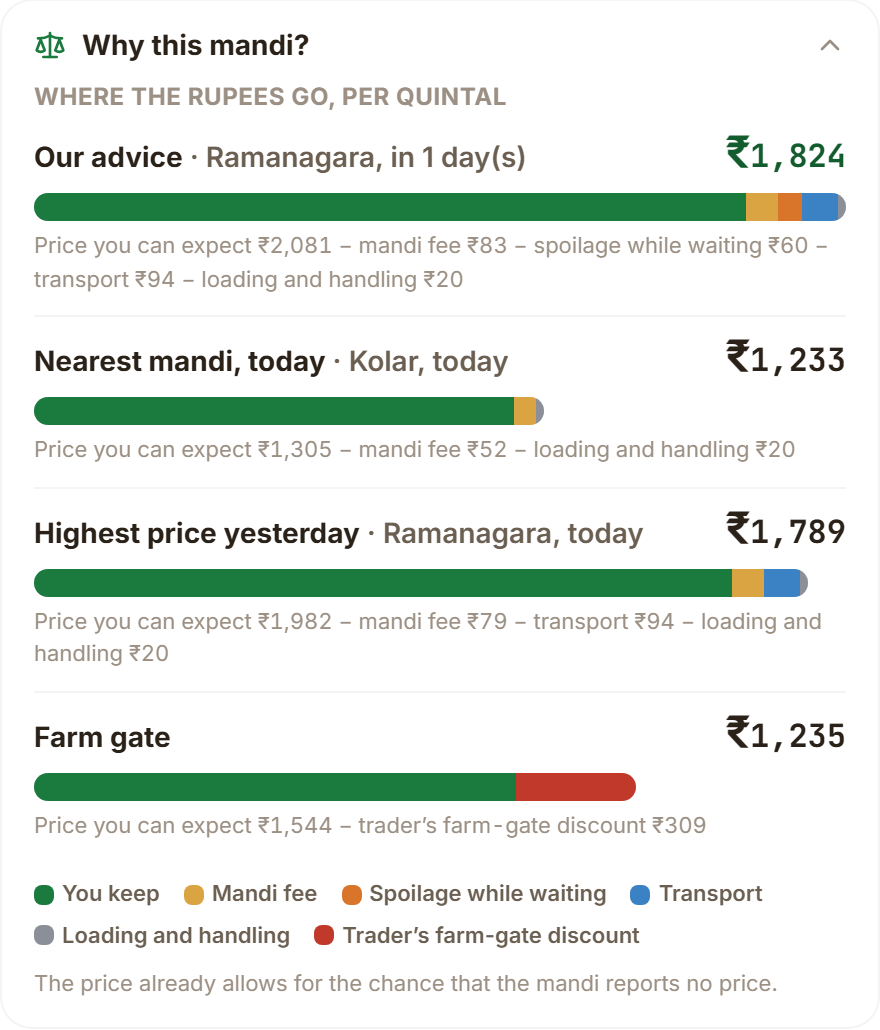
\includegraphics[width=0.94\linewidth]{figures/ins_farmer_why.png}}\\[1mm]{\small (a) Why this mandi?}\end{minipage}\hfill
\begin{minipage}[t]{0.485\textwidth}\centering\fbox{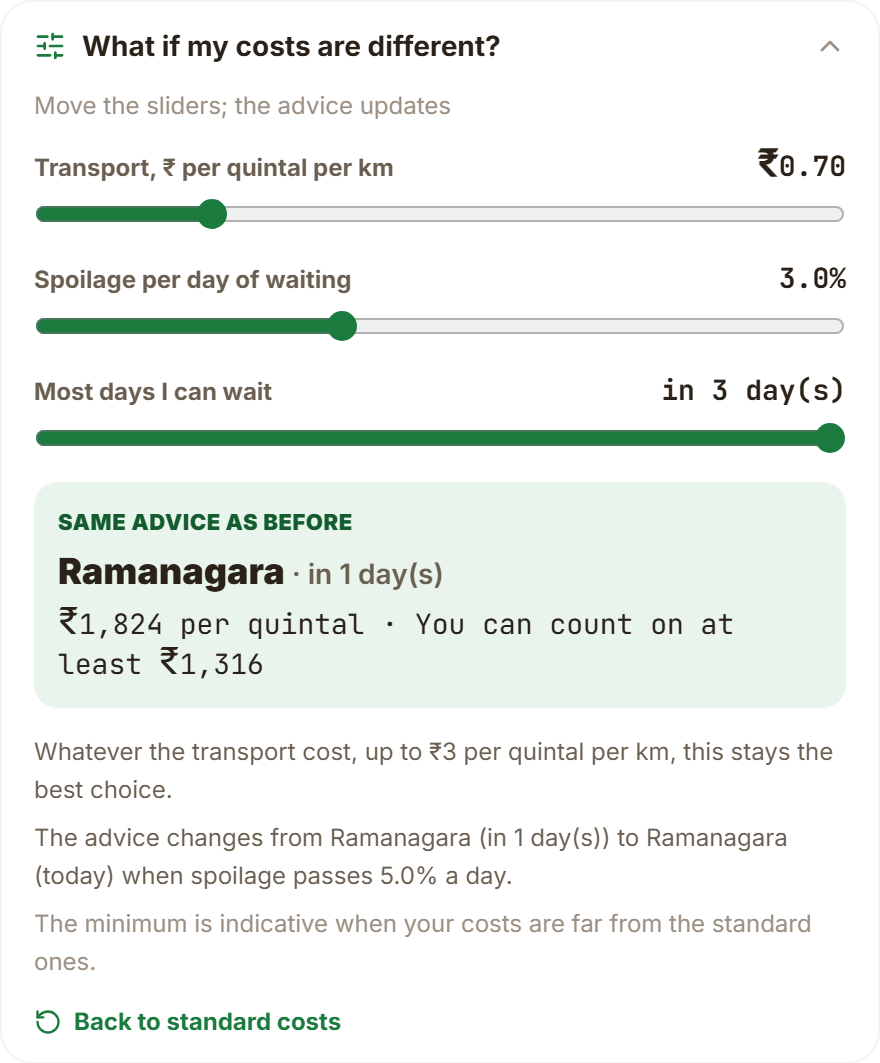
\includegraphics[width=0.94\linewidth]{figures/ins_farmer_whatif.png}}\\[1mm]{\small (b) What if my costs differ?}\end{minipage}
\medskip
\begin{minipage}[t]{0.485\textwidth}\centering\fbox{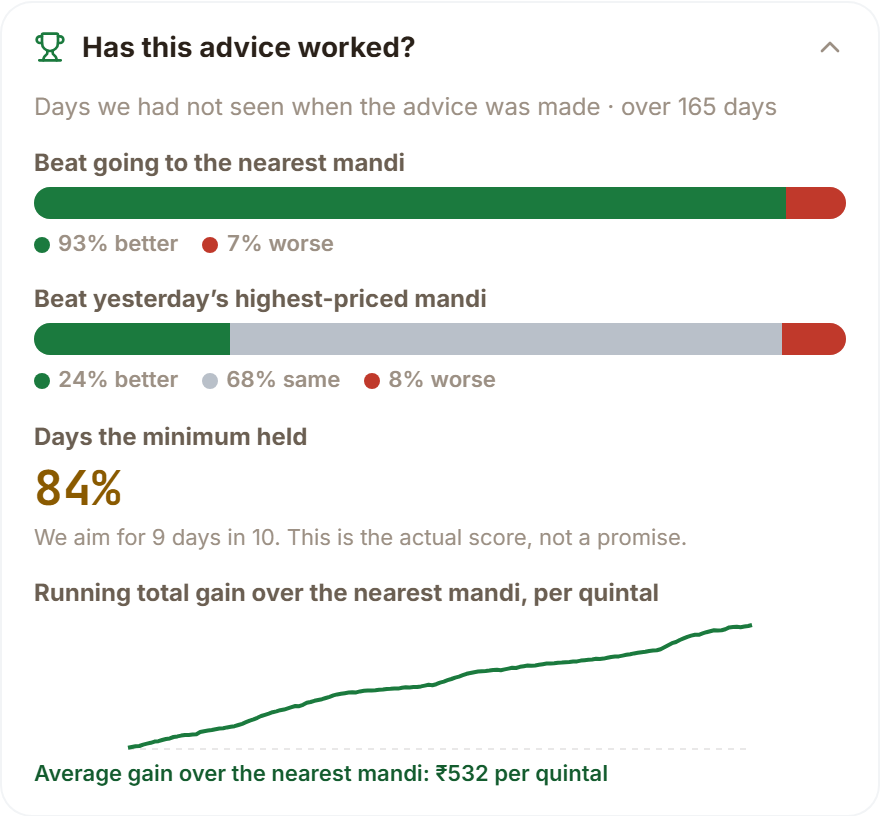
\includegraphics[width=0.94\linewidth]{figures/ins_farmer_score.png}}\\[1mm]{\small (c) Has this advice worked?}\end{minipage}
\caption{The three farmer panels inside the Best Place and Day to Sell tool, for tomato in Kolar, with real data. In (b) the advice changes when spoilage passes 5\% a day.}
\label{fig:ui-insight}
\end{figure}

\subsection{Daily digest and Telegram bot}

The digest builder (\texttt{mandisense\_ai/notify/digest.py}) turns the panel and the engines into one message (Section~\ref{sec:digest-method}). The bot (\texttt{mandisense\_ai/notify/telegram.py}) uses the Telegram Bot API over HTTPS with long polling, so it runs on a laptop with no public address. A farmer presses Start, chooses a language, a district and crops with buttons and receives the first digest at once; \texttt{/today} repeats it, \texttt{/stop} unsubscribes, and typing a crop and a place (``tomato kolar'', or the same in Kannada or Hindi) returns the digest for them. Subscribers and an append-only log of every attempt (sent, failed, with message identifiers) are kept in two files beside the other farmer stores, and a blocked bot marks the subscriber inactive. A script (\texttt{scripts/send\_daily\_digest.py}) sends the morning digest to every active subscriber and has a dry-run mode; scheduled for 07:00 it is the daily message. The bot's token is read from the environment, never logged or committed.

\subsection{Use of AI assistance}
\label{sec:ai-disclosure}
The authors used Anthropic's Claude~\cite{claude3} through the Claude Code command-line assistant as a development and writing aid: for drafting and refactoring code, writing tests, generating the figures and tables from stored experiment results, searching and checking bibliographic records against public indices, and drafting and copy-editing text. The design decisions, experiments, numbers and conclusions are the authors' own; every number in the thesis is produced by scripts from stored artefacts, and every reference was checked against Crossref or arXiv before it was listed. The product itself does not call Claude: its explanation writer and judge are the open-weight models named in Section~\ref{sec:llm}.

\section{System Integration}
\label{sec:system-integration}

\subsection{Pipeline}

One script (\texttt{scripts/pipeline.py}) runs the stages in dependency order: building the farmer world, seeding and running forecasts, building the market-choice engines, the day-by-day track record of the advice, transmission, shock study, spillover, council evaluation, research evidence export, results document, and (optionally) the full research experiments and LLM evaluation, ending with the tests. Each stage is a command with declared outputs, so a stage can be run alone, skipped, or dry-run. Figure~\ref{fig:integration-flow} shows the flow.

\begin{figure}[!t]
\centering
\begin{tikzpicture}[node distance=4mm and 5mm, every node/.style={font=\scriptsize}, s/.style={draw, rounded corners=2pt, fill=blue!6, minimum width=1.9cm, minimum height=7mm, align=center}]
\node[s] (w) {world};
\node[s, right=of w] (f) {forecasts};
\node[s, right=of f] (m) {market\\choice};
\node[s, right=of m] (tr) {track\\record};
\node[s, right=of tr] (t) {transmission};
\node[s, below=of w] (sh) {shock};
\node[s, right=of sh] (sp) {spillover};
\node[s, right=of sp] (c) {council};
\node[s, right=of c] (r) {research\\evidence};
\node[s, below=of sp] (res) {results\\document};
\node[s, right=of res] (te) {tests};
\draw[->] (w)--(f); \draw[->] (f)--(m); \draw[->] (m)--(tr); \draw[->] (tr)--(t);
\draw[->] (t.south) -- ++(0,-0.35) -| (sh.north);
\draw[->] (sh)--(sp); \draw[->] (sp)--(c); \draw[->] (c)--(r);
\draw[->] (r.south) |- (res.east); \draw[->] (res)--(te);
\end{tikzpicture}
\caption{Stages of the reproducible pipeline, in the order they run.}
\label{fig:integration-flow}
\end{figure}

\subsection{Service and application}
\label{sec:service-app}

The FastAPI application mounts routers for market choice (\texttt{/v1/market-choice}), farmer tools (\texttt{/v1/farmer}), trader tools (\texttt{/v1/trader}), supply shocks (\texttt{/v1/shock}), the council (\texttt{/v1/council}), cross-commodity spillover (\texttt{/v1/spillover}), forecasts, chat, decision intelligence (\texttt{/v1/intelligence}), the five insight endpoints under \texttt{/v1/market-choice}, and the notification routes (\texttt{/v1/notify}). Request and response models are typed with Pydantic, so a malformed request is rejected before it reaches a model. The Next.js application calls these endpoints; Figure~\ref{fig:ui-farmer} shows the farmer home in Kannada and the market-choice desk for traders.

\begin{figure}[!t]
\centering
\begin{minipage}[c]{0.27\textwidth}\centering
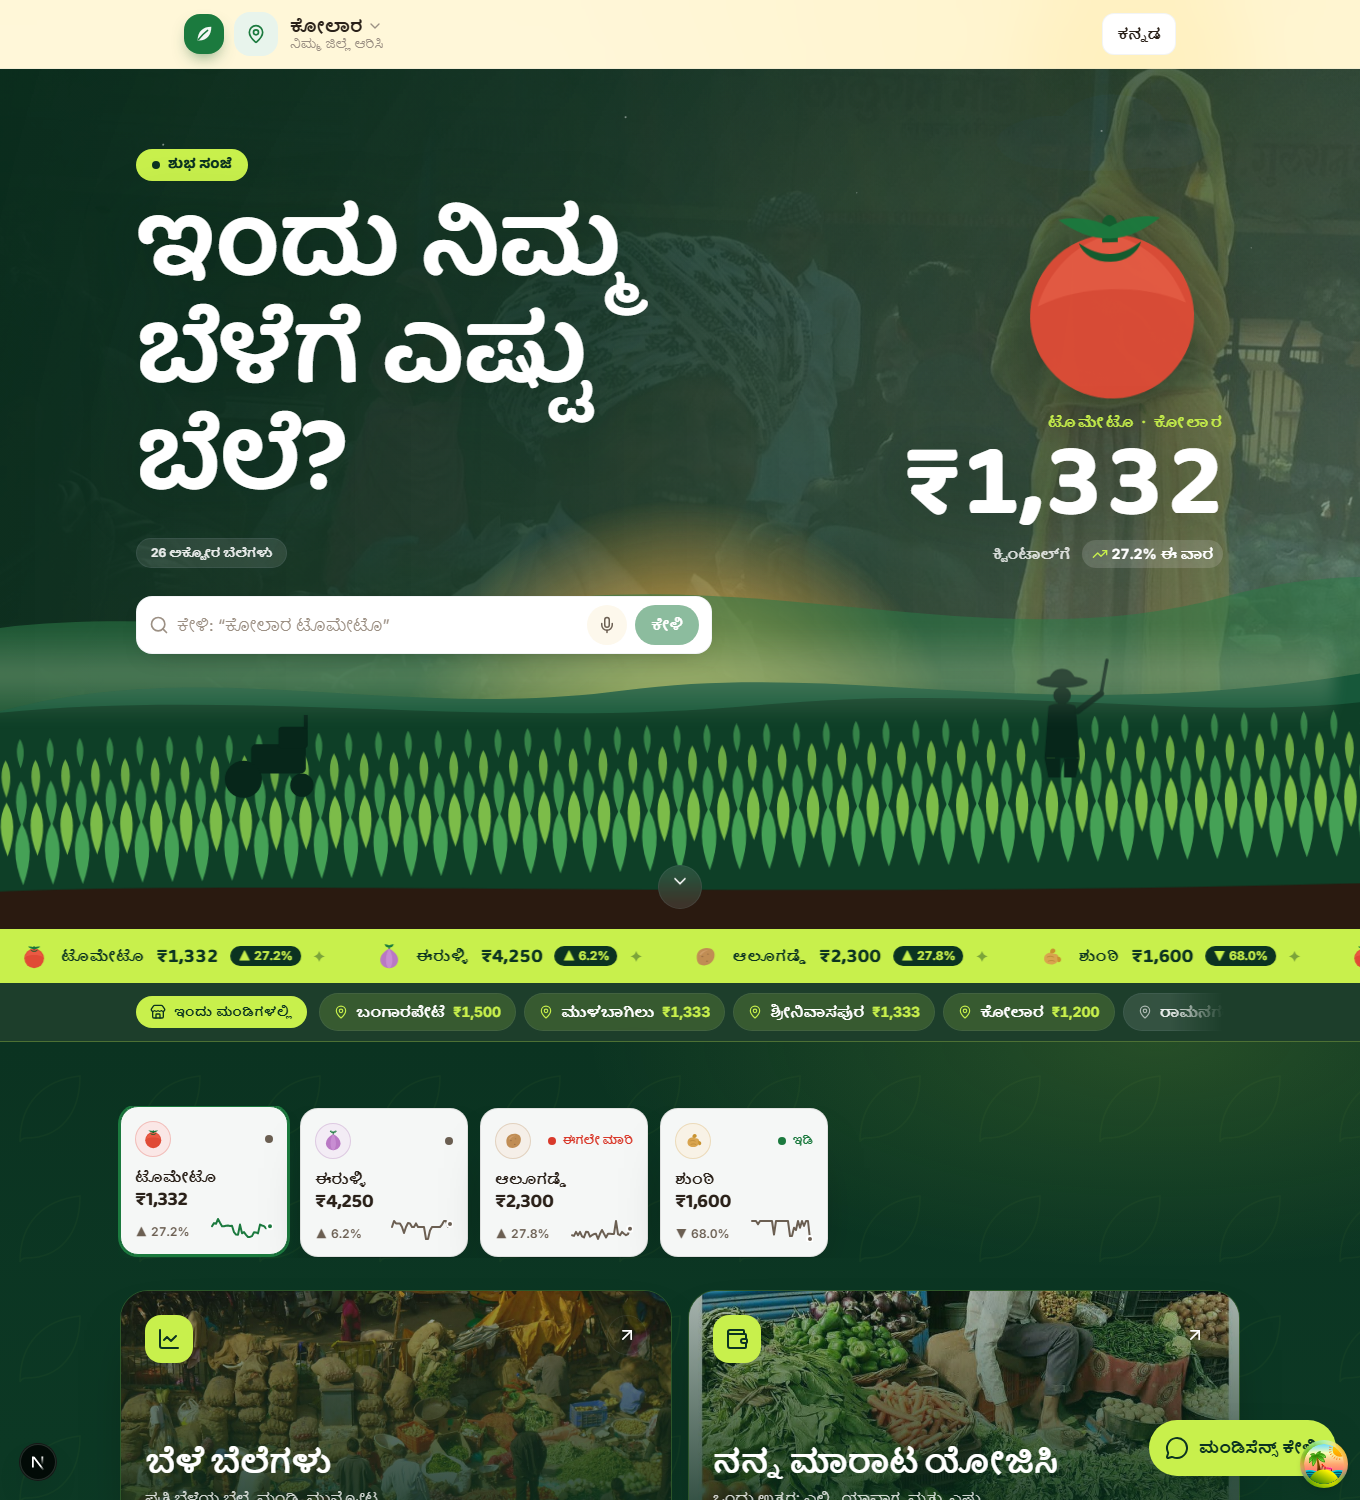
\includegraphics[height=10.4cm]{figures/ui_farmer_home.png}\\[1mm]{\small (a) Farmer home, Kannada}
\end{minipage}\hfill
\begin{minipage}[c]{0.70\textwidth}\centering
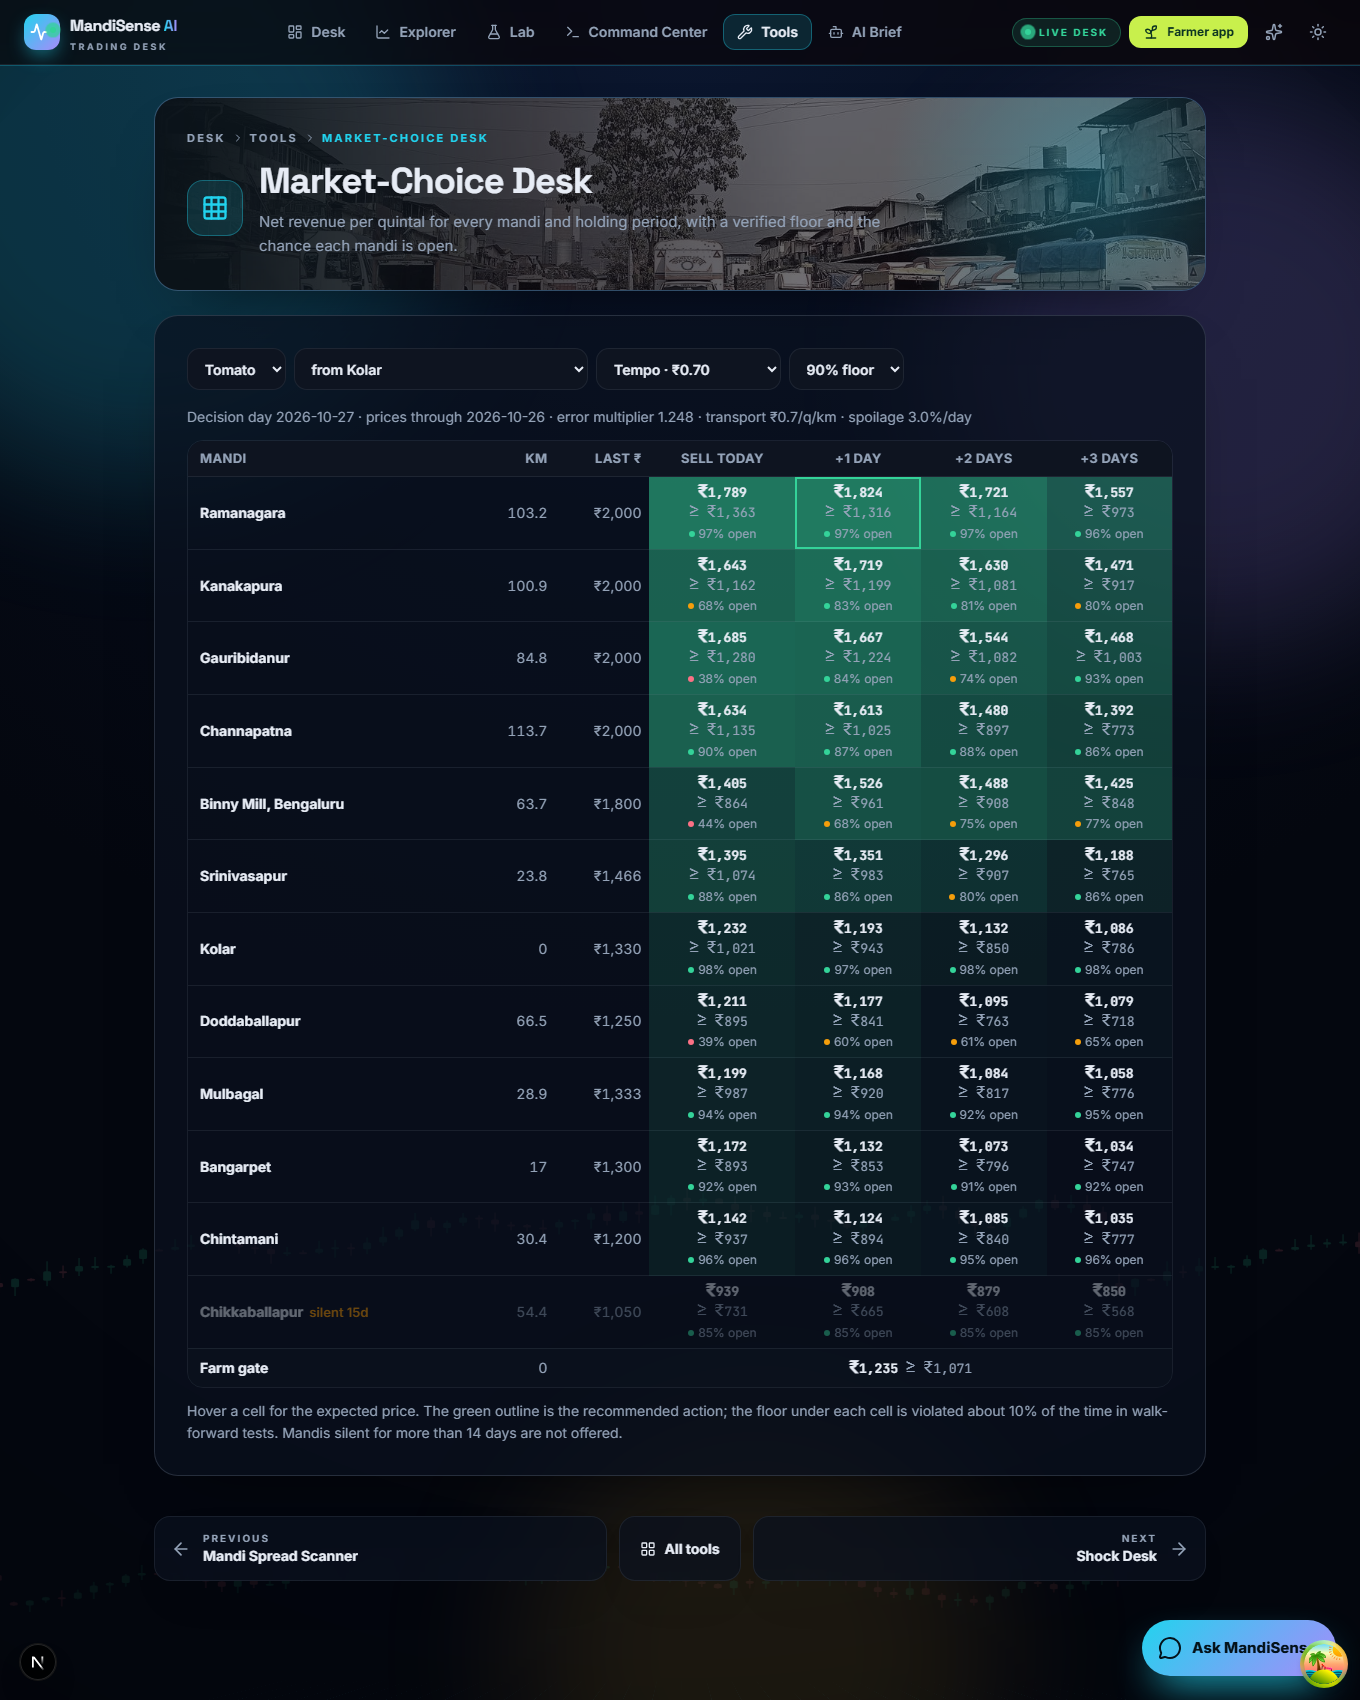
\includegraphics[width=\textwidth]{figures/ui_market_choice.png}\\[1mm]{\small (b) Market-choice desk}
\end{minipage}
\caption{(a) The farmer home screen in Kannada, showing today's best place to sell and the reasons for it. (b) The market-choice desk for traders: recommended market and holding period, the verified floor and the evidence level for the crop. Both are rendered from real data.}
\label{fig:ui-farmer}
\end{figure}

\subsection{Challenges and solutions}
Table~\ref{tab:challenges} lists the integration problems met while joining the parts and how each was resolved.

\begin{table}[H]
\centering
\caption{Integration problems met and how they were resolved}
\label{tab:challenges}
\small
\begin{tabular}{|p{4.6cm}|p{5.2cm}|p{4.6cm}|}
\hline
\textbf{Problem} & \textbf{Cause} & \textbf{Resolution} \\ \hline
Pandas failed to import after installing a plotting library & The installer upgraded NumPy to 2.5, incompatible with pandas 2.1.4 & Pinned NumPy 1.26.4; regenerated the lock file; dependency check clean \\ \hline
Ginger experiment found no rows & Export names the crop ``Ginger(Green)'' & Added a source-name alias in the configuration \\ \hline
Fresh clone failed three tests and skipped four & The observation store was untracked & Tracked the store; pipeline seeds history; tests guarded \\ \hline
Trader pages empty after a data refresh & Hard deletion of records broke references & Re-seeding and id aliasing \\ \hline
Council weights summed to more than 1 & Unconstrained non-negative least squares & Constrained sum to at most one; unconstrained kept as a reported column \\ \hline
Language-layer calls throttled & Provider limit of 8,000 tokens per minute & Request throttling; small evaluation set \\ \hline
Silence tax read as zero for a cheap, unreliable mandi & Its usual price is below the fallback price, so silence costs no money on price & Added a surprise-silence column and a note that zero is not reliability \\ \hline
New endpoints answered ``not found'' in testing & A server started before the change was still running old code & Restarted it; the smoke test lists every new endpoint and page \\ \hline
\end{tabular}
\end{table}

\section{System Walkthrough with Screenshots}
\label{sec:screens}

This section shows the running system. Every figure is a screenshot of the web application served from the stored data of the final system (market prices up to 26 October 2026), captured by a script (\texttt{report/capture\_system.py}) driving a headless browser, so the figures can be regenerated and are not edited. The farmer interface is shown at phone width because that is how most farmers will use it; the trader desk is shown at desktop width. Prices are in rupees per quintal unless stated, and every price on screen carries the date it was reported.

\subsection{Farmer interface}
The farmer interface is built around a single question, ``what is my crop worth today, and where should I sell it?''. It has a language switch (English, Kannada, Hindi), a district selector and a bottom navigation bar with Home, Prices and Tools.


\begin{figure}[!t]
\centering
\begin{minipage}[t]{0.485\textwidth}\centering\fbox{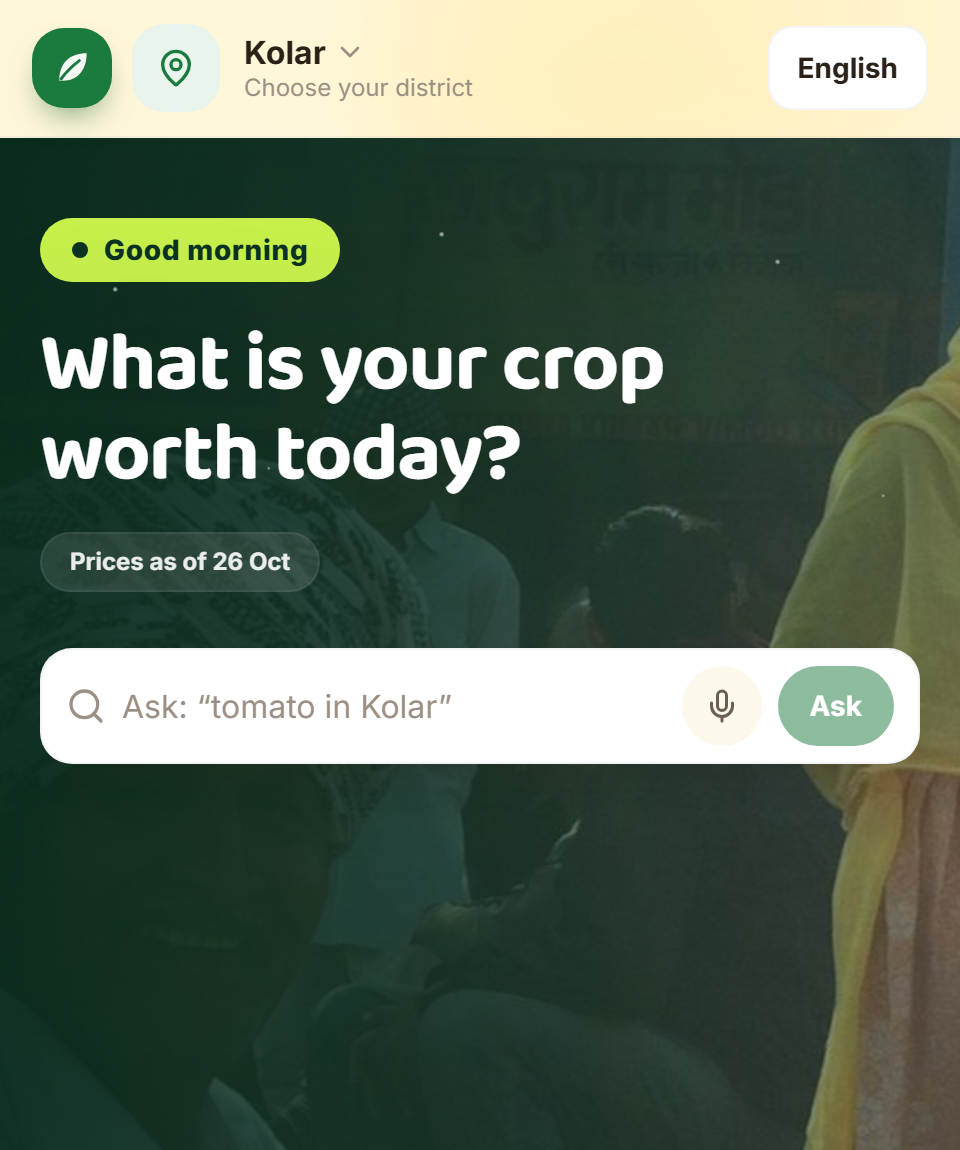
\includegraphics[width=0.94\linewidth,height=9.0cm,keepaspectratio]{figures/shot_f_home.png}}\\[1mm]{\footnotesize (a) Home}\end{minipage}\hfill
\begin{minipage}[t]{0.485\textwidth}\centering\fbox{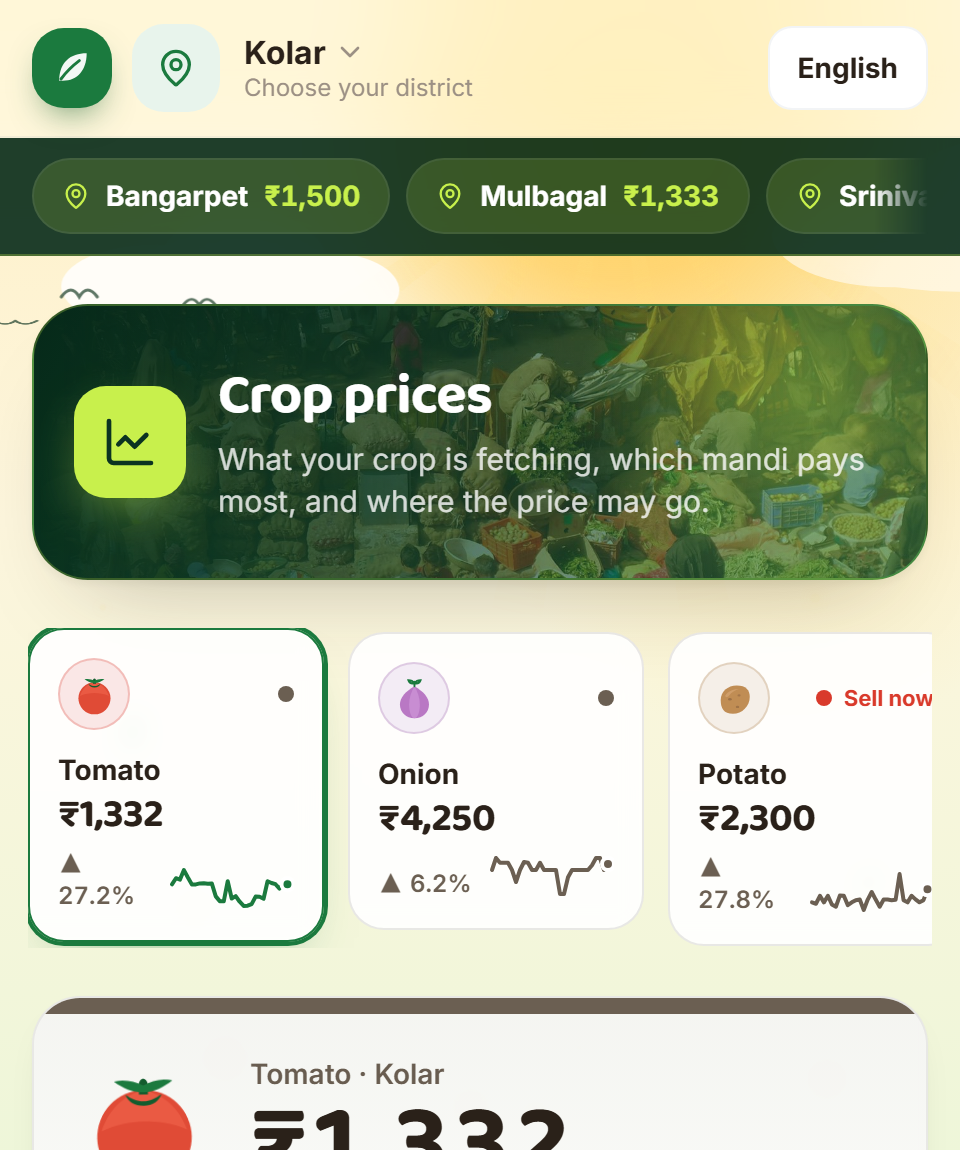
\includegraphics[width=0.94\linewidth,height=9.0cm,keepaspectratio]{figures/shot_f_prices.png}}\\[1mm]{\footnotesize (b) Prices}\end{minipage}
\medskip
\centering \begin{minipage}[t]{0.485\textwidth}\centering\fbox{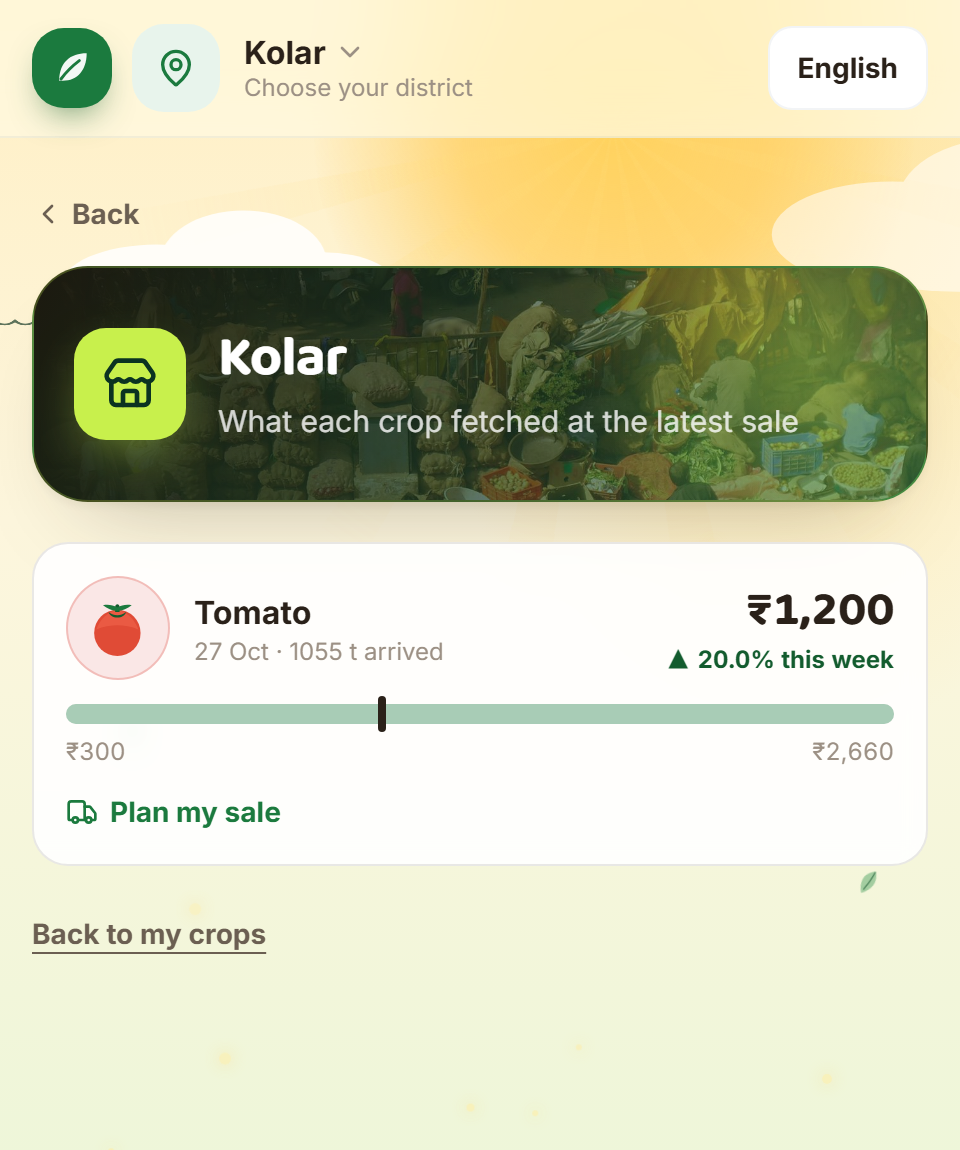
\includegraphics[width=0.94\linewidth,height=9.0cm,keepaspectratio]{figures/shot_f_mandi.png}}\\[1mm]{\footnotesize (c) One mandi}\end{minipage}
\caption{Farmer pages. (a) The home page opens with a plain question, a search box that answers in sentences, and a ticker of the latest prices. (b) The prices page lists the crops with the latest quote, the change over the week and a sparkline. (c) A mandi page shows what each crop fetched there at the latest sale and how many quintals arrived.}
\label{fig:sc-farmer1}
\end{figure}

The home page (Figure~\ref{fig:sc-farmer1}a) deliberately carries no table: the first thing a farmer sees is the question and a box in which to type one in ordinary words. The prices page (b) shows the quote for each crop together with the date of the last report, so a stale price is never presented as today's. The mandi page (c) is the farmer-side view of one market and links to the plan for selling there.


\begin{figure}[!t]
\centering
\begin{minipage}[t]{0.485\textwidth}\centering\fbox{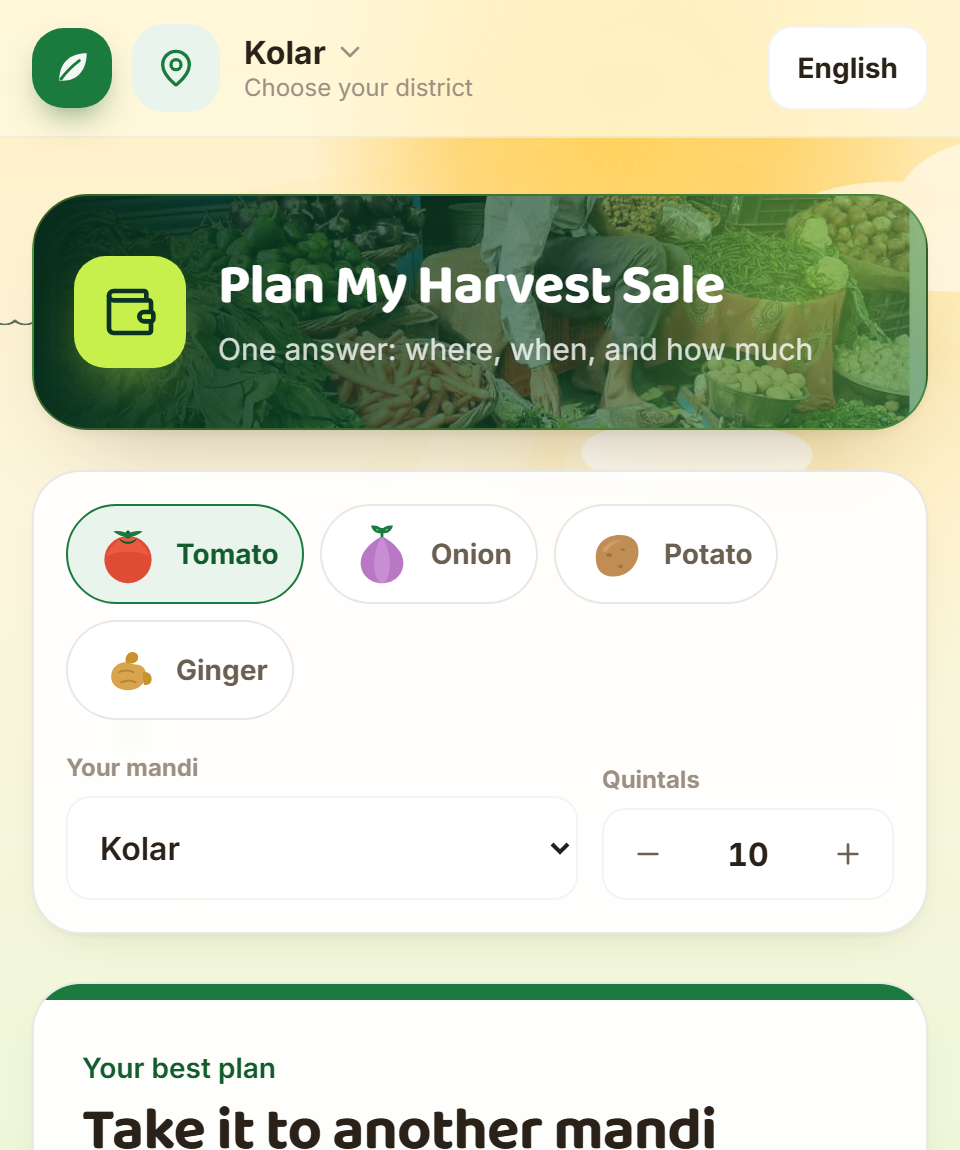
\includegraphics[width=0.94\linewidth,height=9.0cm,keepaspectratio]{figures/shot_f_sellplan.png}}\\[1mm]{\footnotesize (a) Plan my sale}\end{minipage}\hfill
\begin{minipage}[t]{0.485\textwidth}\centering\fbox{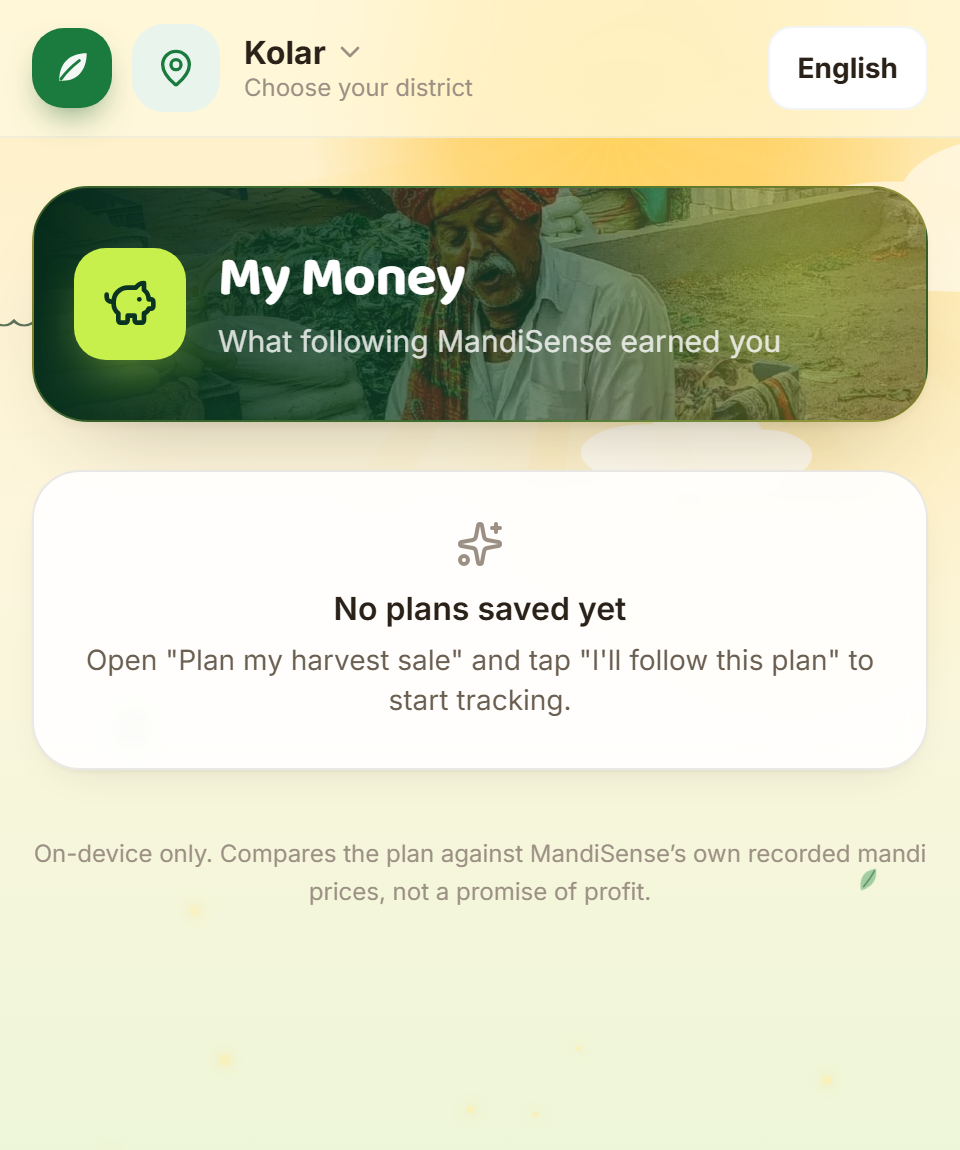
\includegraphics[width=0.94\linewidth,height=9.0cm,keepaspectratio]{figures/shot_f_mymoney.png}}\\[1mm]{\footnotesize (b) My money}\end{minipage}
\medskip
\centering \begin{minipage}[t]{0.485\textwidth}\centering\fbox{
\includegraphics[width=0.94\linewidth,height=9.0cm,keepaspectratio]{figures/shot_f_tools.png}}\\[1mm]{\footnotesize (c) Farmer tools}\end{minipage}
\caption{(a) The sale plan states one recommendation, the amount expected after transport and spoilage, and the day to go. (b) ``My Money'' compares the plans the farmer followed with what the markets recorded; it works on the device only. (c) The tool launcher opens each tool as a sheet over the page.}
\label{fig:sc-farmer2}
\end{figure}

The sale plan (Figure~\ref{fig:sc-farmer2}a) is the product's central screen. It names one market and one day, shows the amount expected per quintal after the cost of moving the crop, and shows the figure the farmer \emph{can count on at least}, which is the revenue floor of Section~\ref{sec:floors}. ``My Money'' (b) keeps the plans on the farmer's phone, so no account or personal data reach the server. The launcher (c) lists the eleven tools whose screens follow.


\begin{figure}[!t]
\centering
\begin{minipage}[t]{0.485\textwidth}\centering\fbox{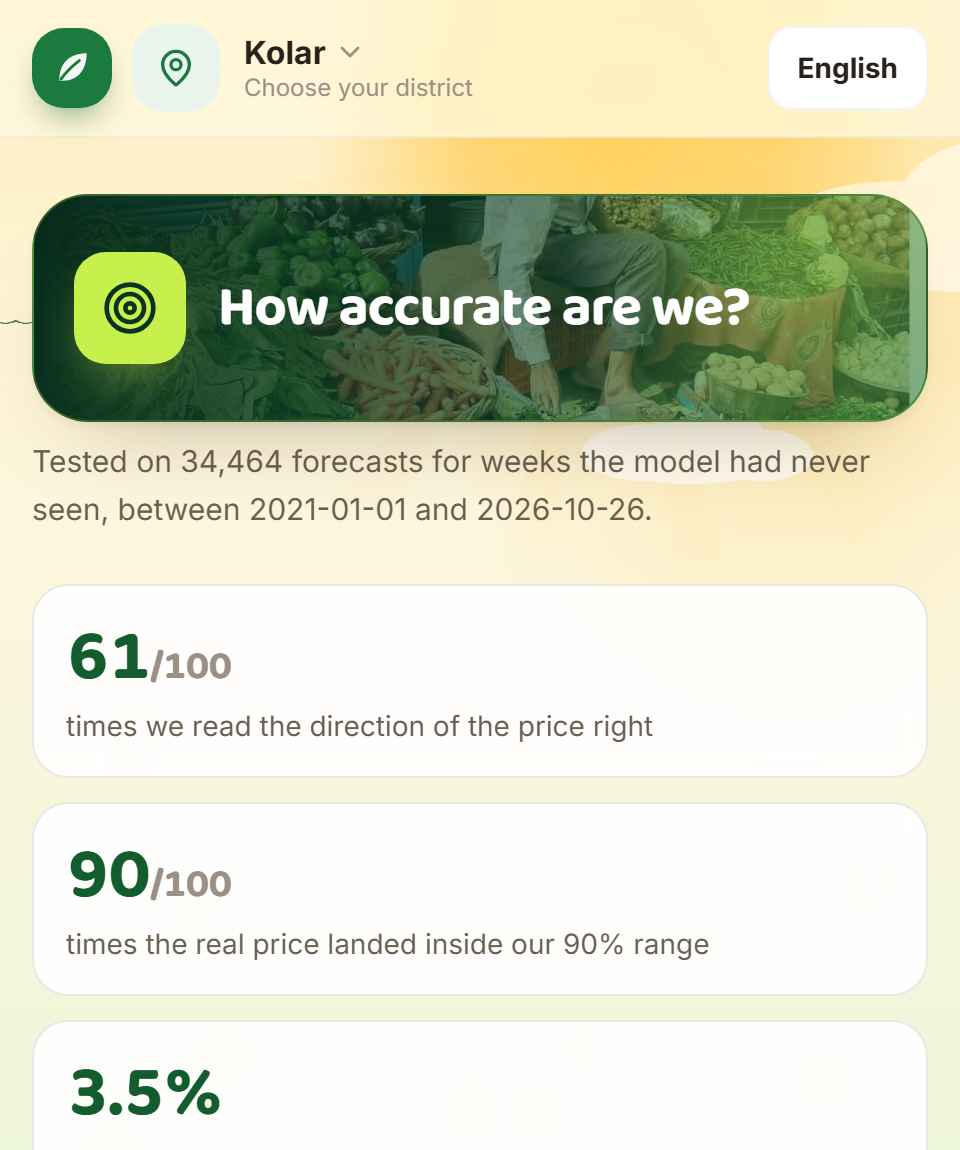
\includegraphics[width=0.94\linewidth,height=9.0cm,keepaspectratio]{figures/shot_f_accuracy.png}}\\[1mm]{\footnotesize (a) How accurate are we?}\end{minipage}\hfill
\begin{minipage}[t]{0.485\textwidth}\centering\fbox{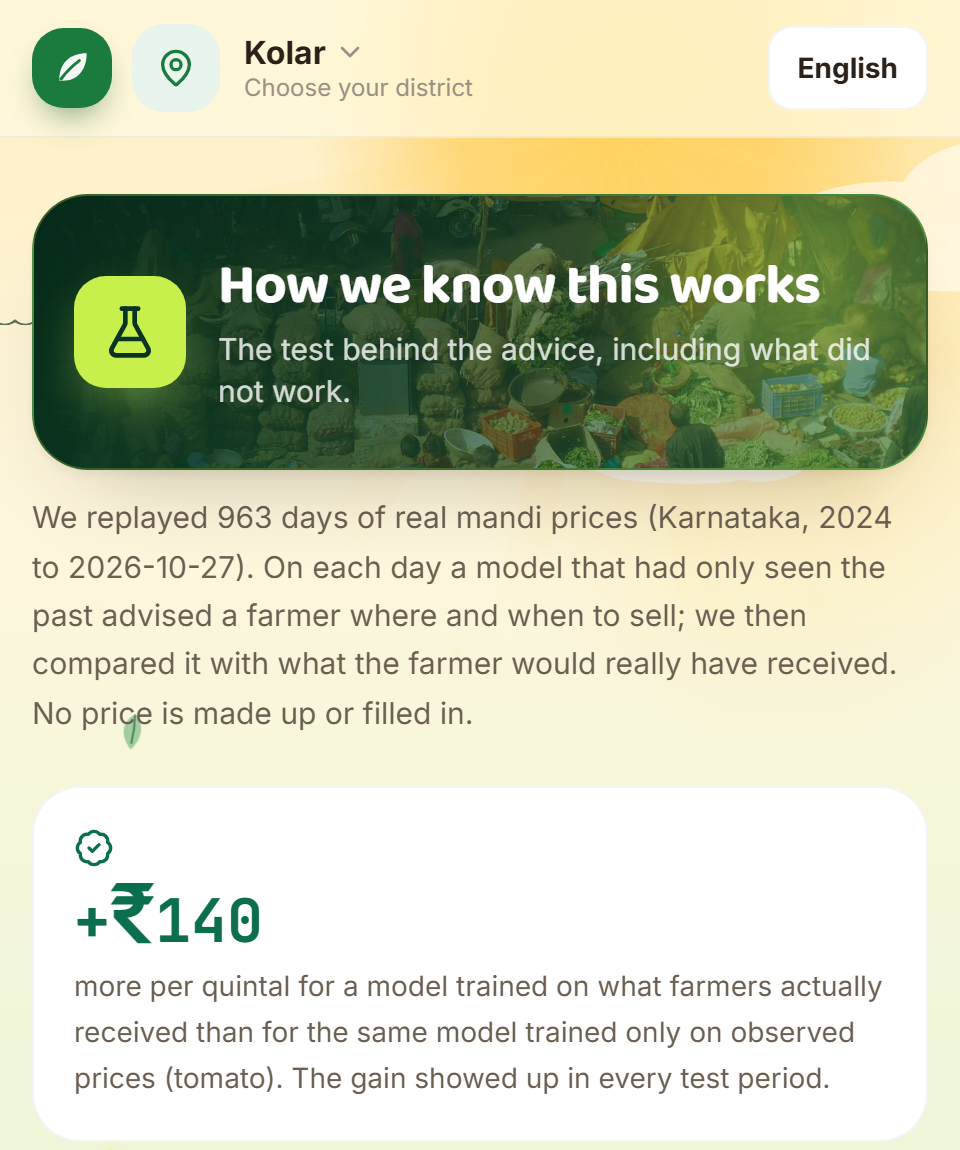
\includegraphics[width=0.94\linewidth,height=9.0cm,keepaspectratio]{figures/shot_f_evidence.png}}\\[1mm]{\footnotesize (b) How we know this works}\end{minipage}
\medskip
\centering \begin{minipage}[t]{0.485\textwidth}\centering\fbox{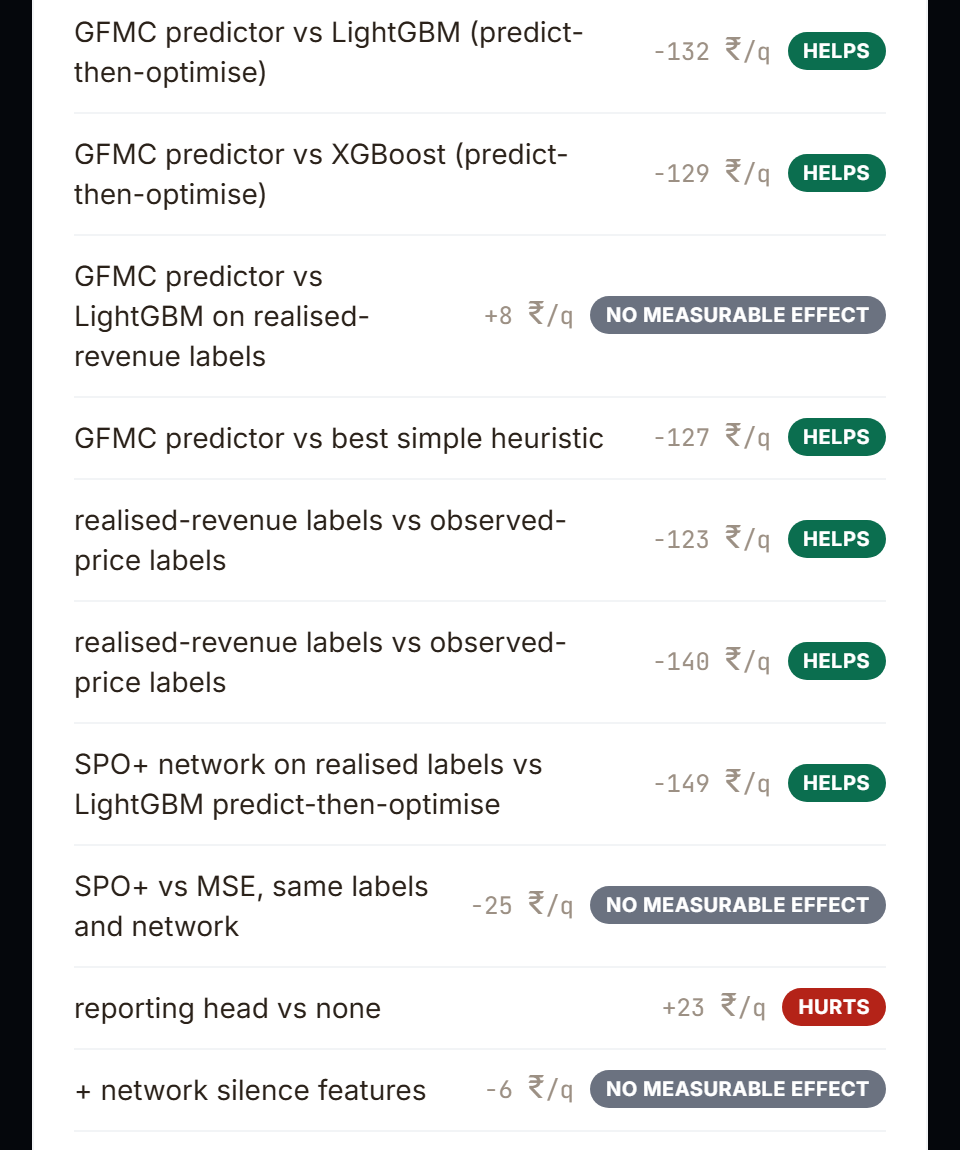
\includegraphics[width=0.94\linewidth,height=9.0cm,keepaspectratio]{figures/shot_f_evidence_b.png}}\\[1mm]{\footnotesize (c) What did not work}\end{minipage}
\caption{The honesty pages. (a) Hit rates by crop and market, on days the system had not seen. (b) The replay: what the method earns against simple alternatives, in rupees, with the seed-to-seed spread. (c) The negative results are listed beside the positive ones.}
\label{fig:sc-farmer3}
\end{figure}

Three pages exist only to let a reader check the system. The accuracy page (Figure~\ref{fig:sc-farmer3}a) reports, per crop and market, how often the advice held on days the system had not seen. The evidence page (b) reproduces the main comparison of Chapter~\ref{ch:results} in plain words and in rupees, and (c) lists what did not help. A product that shows its misses is easier to trust than one that does not.

\subsection{Farmer tools}
Each tool opens as a sheet over the page and answers one question. The sheets below are captured with the sheet in its resting state; the blurred page behind each sheet is cropped away.


\begin{figure}[!t]
\centering
\begin{minipage}[t]{0.485\textwidth}\centering\fbox{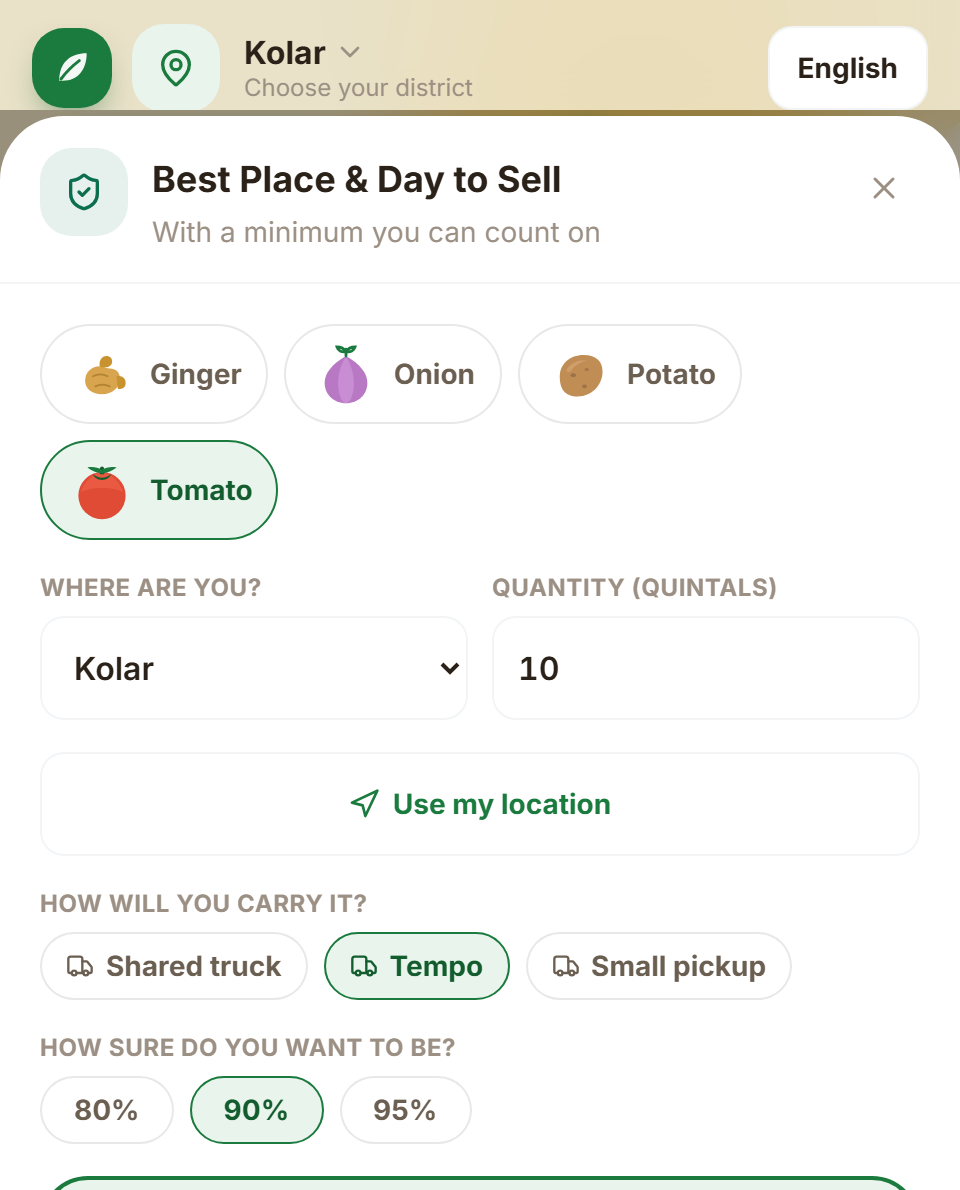
\includegraphics[width=0.94\linewidth,height=9.0cm,keepaspectratio]{figures/shot_t_besplace.png}}\\[1mm]{\footnotesize (a) Best place and day}\end{minipage}\hfill
\begin{minipage}[t]{0.485\textwidth}\centering\fbox{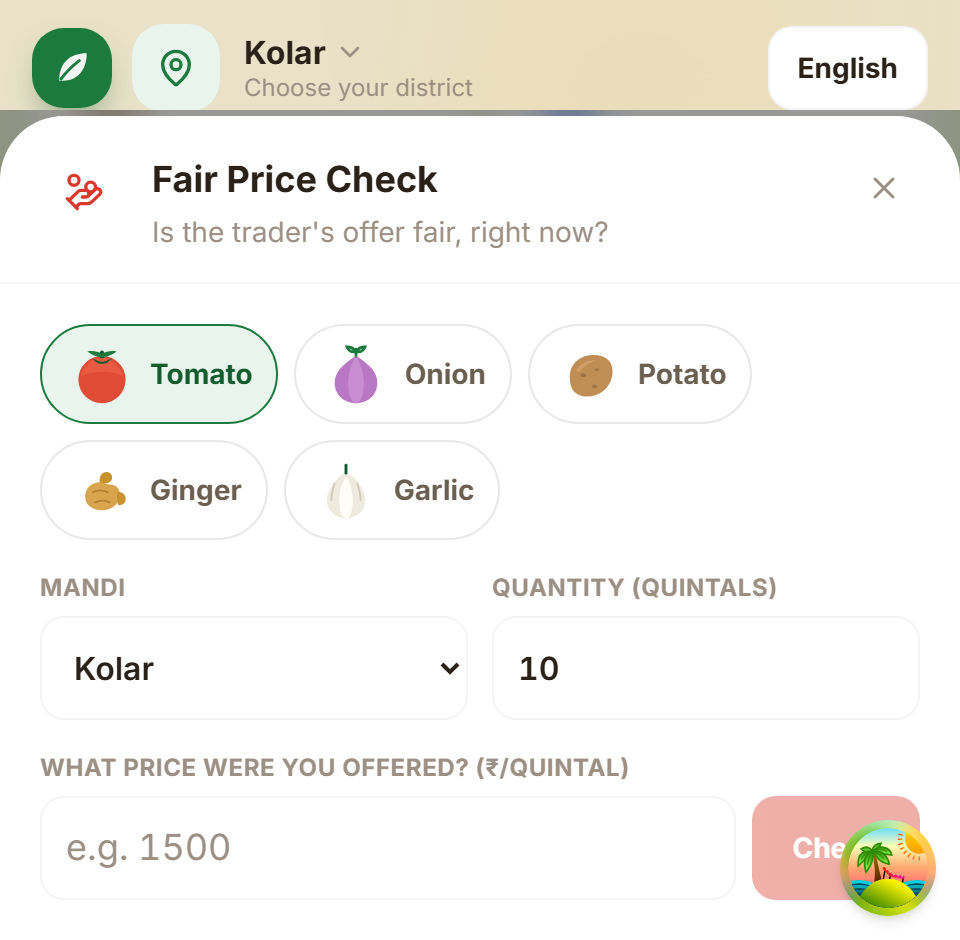
\includegraphics[width=0.94\linewidth,height=9.0cm,keepaspectratio]{figures/shot_t_fairprice.png}}\\[1mm]{\footnotesize (b) Fair price check}\end{minipage}
\medskip
\centering \begin{minipage}[t]{0.485\textwidth}\centering\fbox{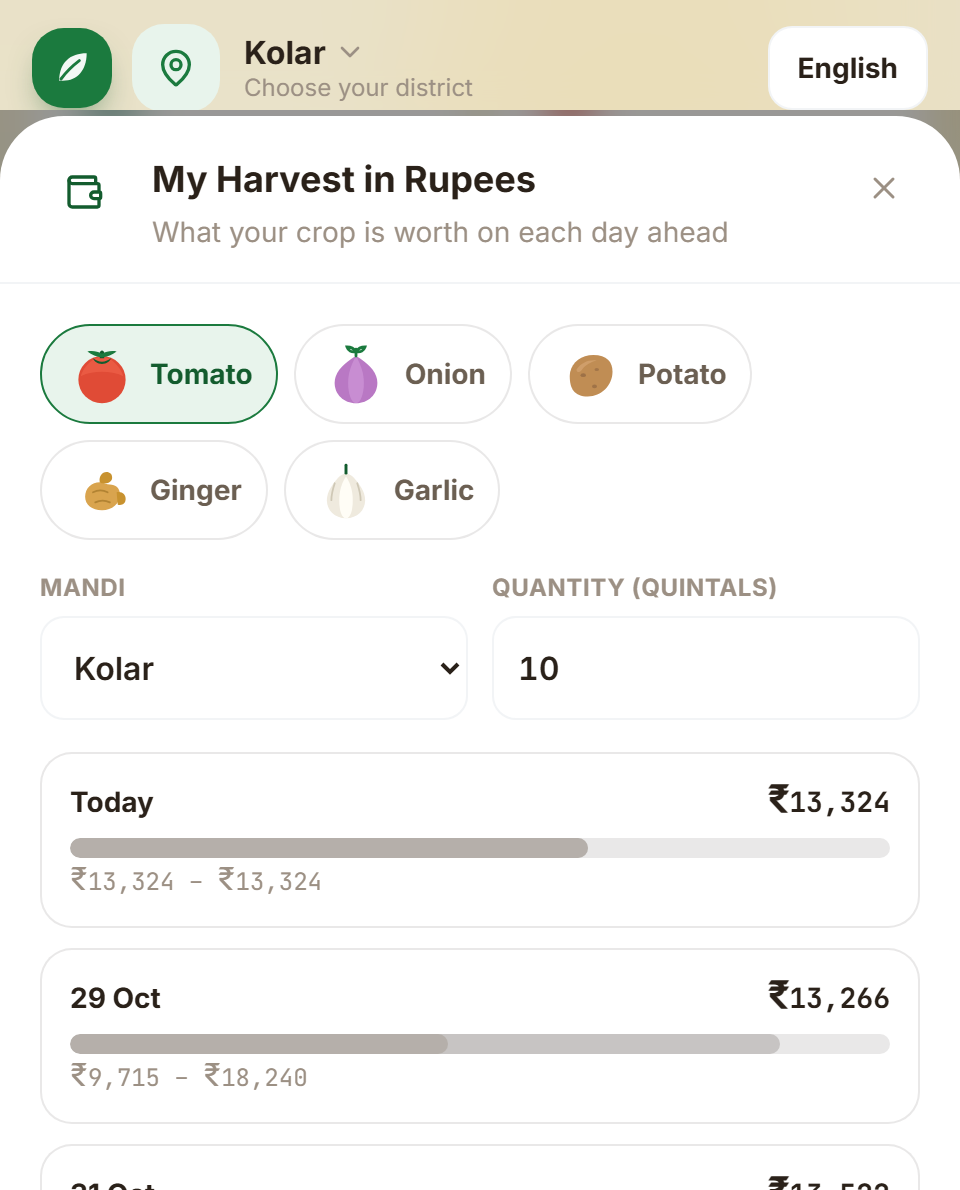
\includegraphics[width=0.94\linewidth,height=9.0cm,keepaspectratio]{figures/shot_t_harvest.png}}\\[1mm]{\footnotesize (c) My harvest in rupees}\end{minipage}
\caption{Selling tools. (a) The recommended market with expected and guaranteed amounts, options to change the vehicle and the confidence, and the next best choices. (b) A check of whether the price a trader offered is fair. (c) The expected value of the crop on each day ahead, after spoilage.}
\label{fig:sc-tools1}
\end{figure}

The Best Place and Day to Sell sheet (Figure~\ref{fig:sc-tools1}a) asks for the district, the quantity, the vehicle and the confidence level (80, 90 or 95\%), and returns the same recommendation as the service of Section~\ref{sec:service-app}, with the cost arithmetic one tap away. The fair-price check (b) takes the offer a trader made and places it against the distribution of recent prices. The harvest sheet (c) lays the next days side by side as a bar for each, with the expected net value, so the farmer sees what waiting costs.


\begin{figure}[!t]
\centering
\begin{minipage}[t]{0.485\textwidth}\centering\fbox{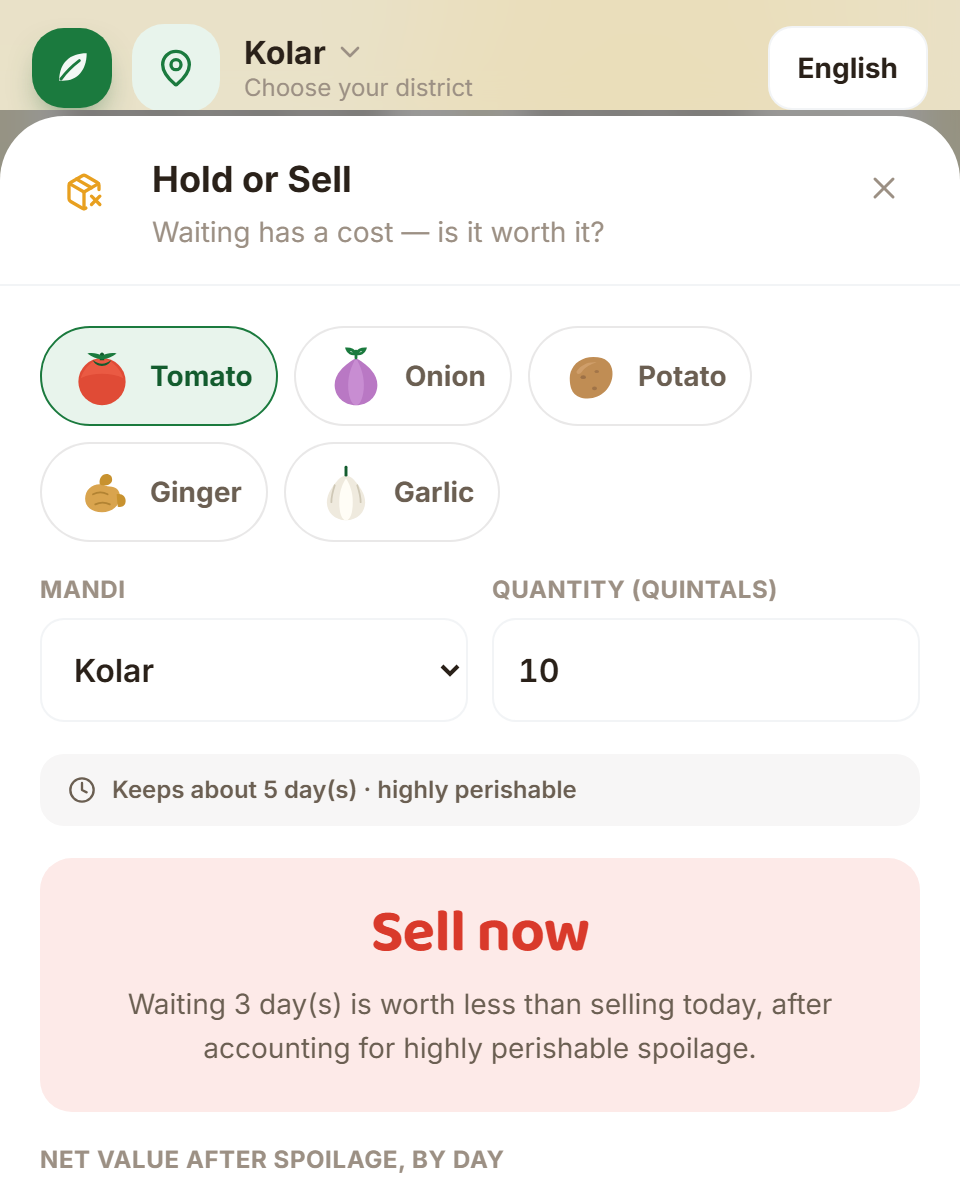
\includegraphics[width=0.94\linewidth,height=9.0cm,keepaspectratio]{figures/shot_t_holdorsell.png}}\\[1mm]{\footnotesize (a) Hold or sell}\end{minipage}\hfill
\begin{minipage}[t]{0.485\textwidth}\centering\fbox{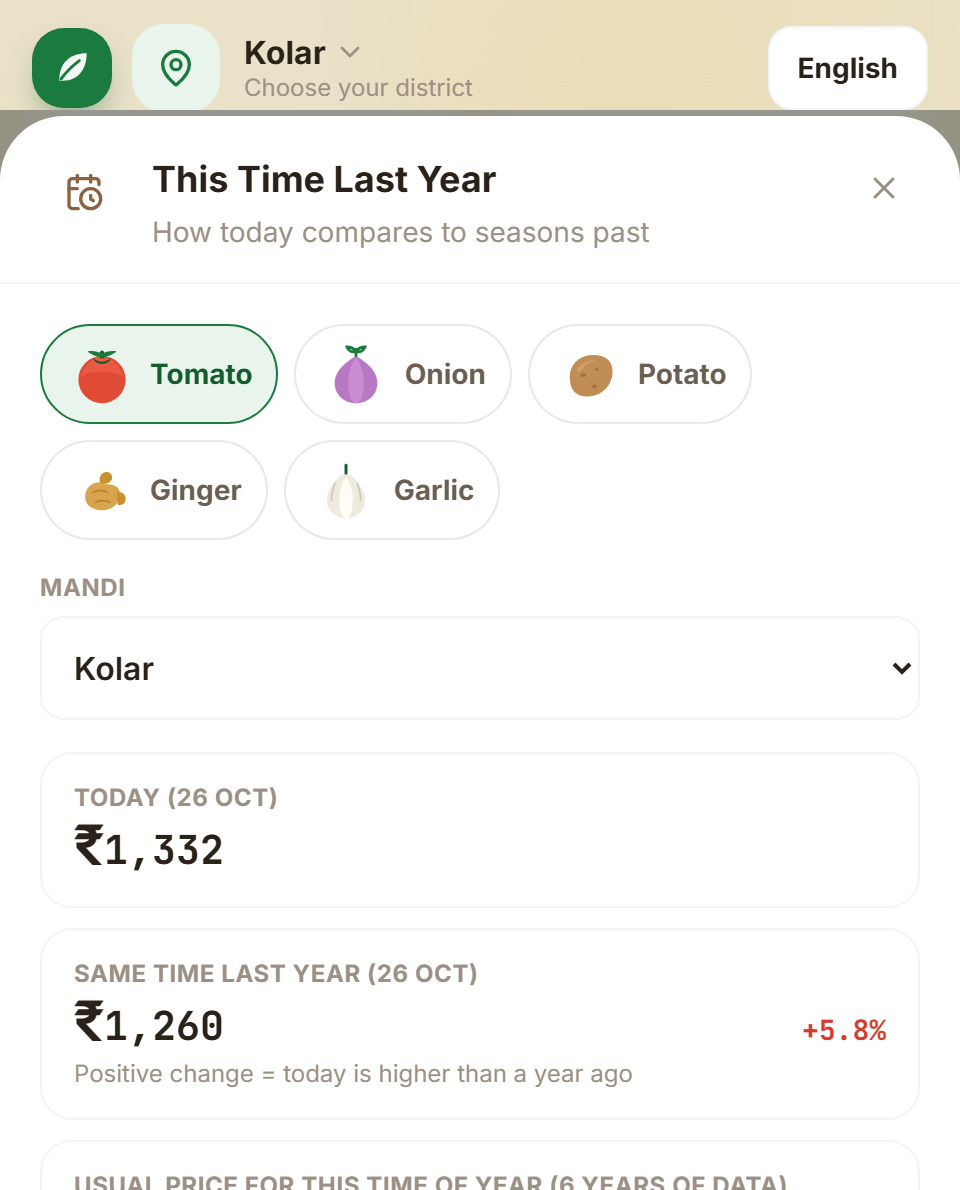
\includegraphics[width=0.94\linewidth,height=9.0cm,keepaspectratio]{figures/shot_t_lastyear.png}}\\[1mm]{\footnotesize (b) This time last year}\end{minipage}
\medskip
\centering \begin{minipage}[t]{0.485\textwidth}\centering\fbox{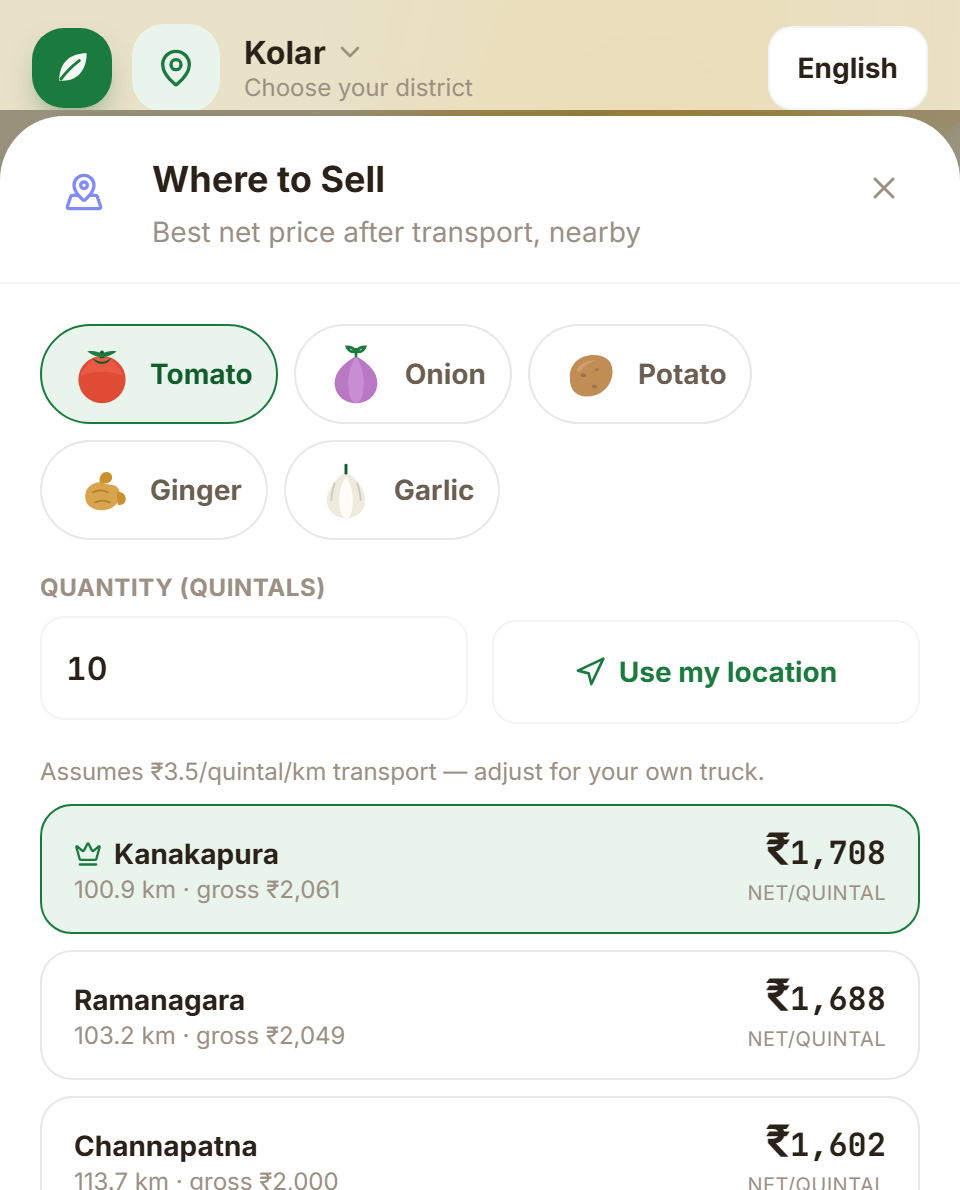
\includegraphics[width=0.94\linewidth,height=9.0cm,keepaspectratio]{figures/shot_t_wheretosell.png}}\\[1mm]{\footnotesize (c) Where to sell}\end{minipage}
\caption{Timing and location tools. (a) A hold-or-sell call that weighs spoilage against the expected price gain. (b) Today's price against the same date last year and the seasonal norm. (c) Nearby markets ranked by price after transport.}
\label{fig:sc-tools2}
\end{figure}

Hold or Sell (Figure~\ref{fig:sc-tools2}a) is built for the perishable case: it states the cost of waiting a day, so that ``wait'' is never the free option it appears to be. The seasonal sheet (b) gives context, not a forecast, and is labelled so. The ranking (c) lists markets with distance, gross price and net price per quintal under an assumed transport cost that the farmer can change.


\begin{figure}[!t]
\centering
\begin{minipage}[t]{0.485\textwidth}\centering\fbox{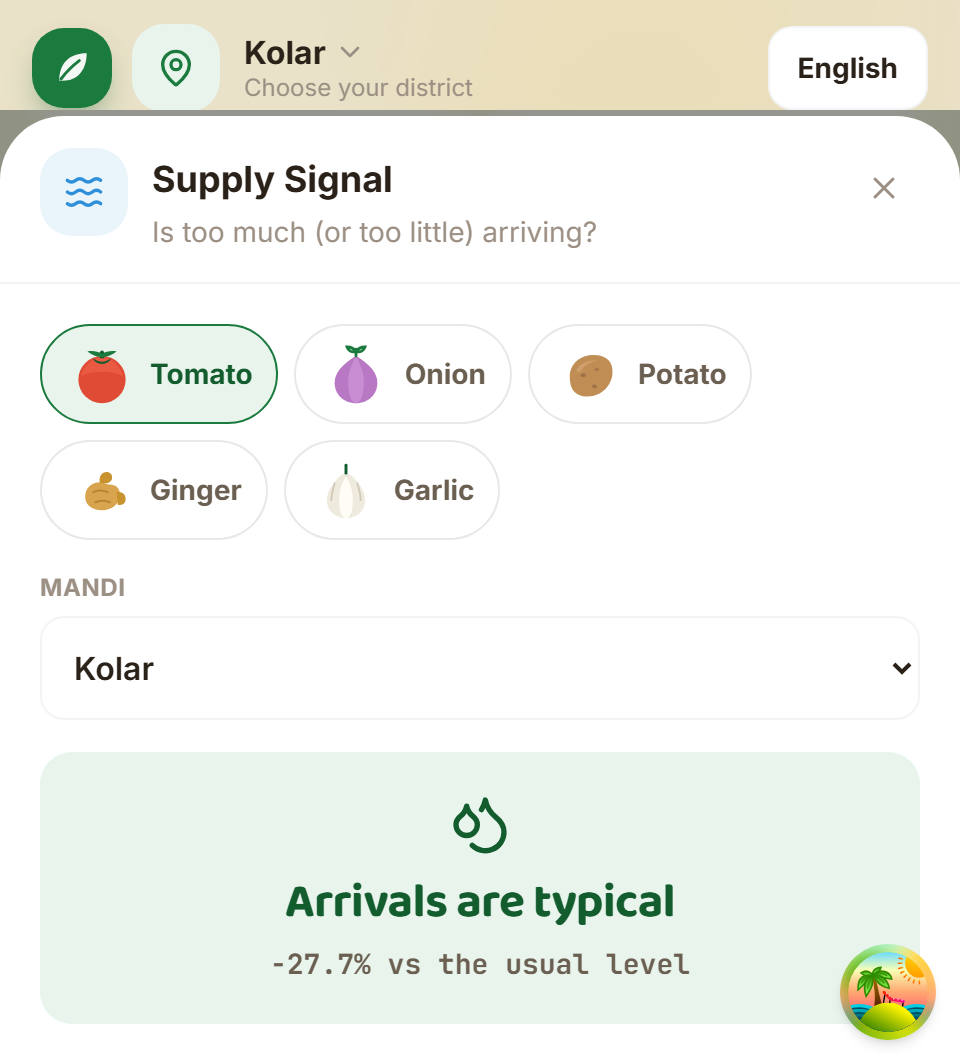
\includegraphics[width=0.94\linewidth,height=9.0cm,keepaspectratio]{figures/shot_t_supply.png}}\\[1mm]{\footnotesize (a) Supply signal}\end{minipage}\hfill
\begin{minipage}[t]{0.485\textwidth}\centering\fbox{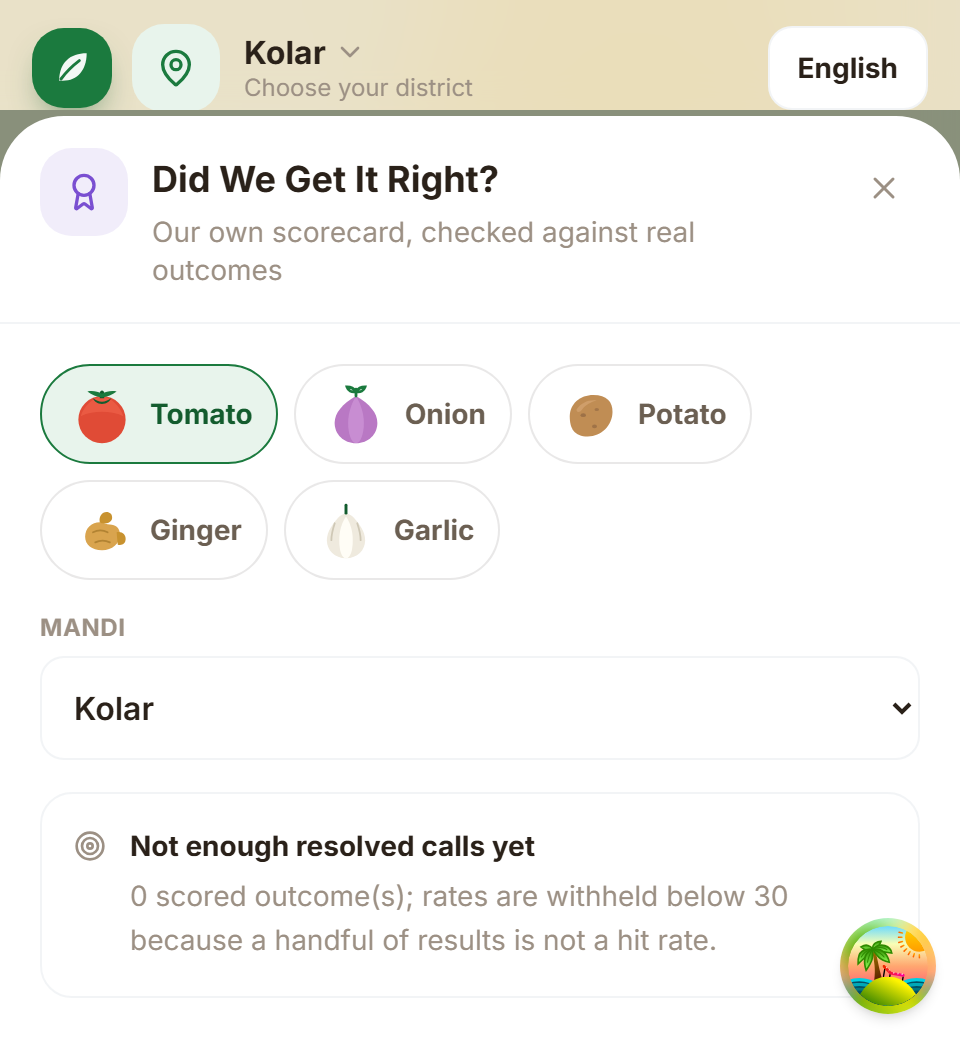
\includegraphics[width=0.94\linewidth,height=9.0cm,keepaspectratio]{figures/shot_t_record.png}}\\[1mm]{\footnotesize (b) Did we get it right?}\end{minipage}
\medskip
\centering \begin{minipage}[t]{0.485\textwidth}\centering\fbox{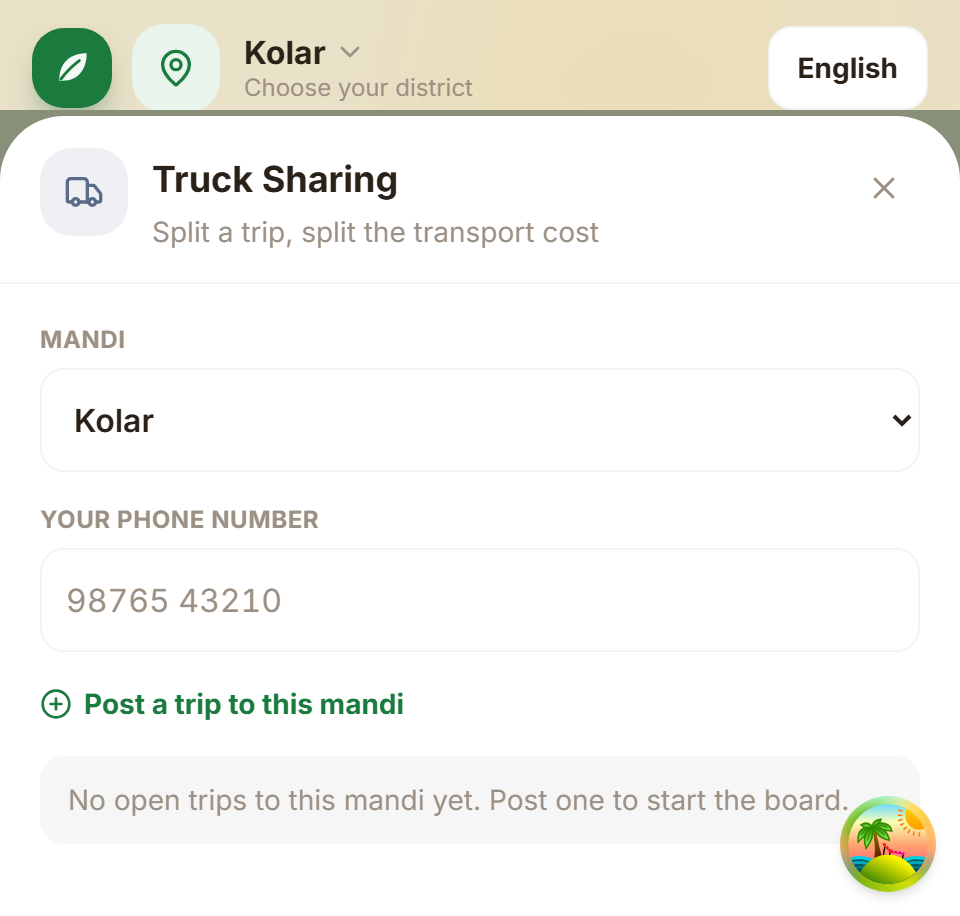
\includegraphics[width=0.94\linewidth,height=9.0cm,keepaspectratio]{figures/shot_t_truck.png}}\\[1mm]{\footnotesize (c) Truck sharing}\end{minipage}
\caption{Context and sharing tools. (a) Arrivals against the usual level. (b) The system's own scorecard of resolved calls. (c) A board for splitting a truck to a market.}
\label{fig:sc-tools3}
\end{figure}

The supply signal (Figure~\ref{fig:sc-tools3}a) reports whether arrivals are unusually high or low, since a glut lowers price. The scorecard (b) is an honest counter: when too few calls have resolved it says so and withholds the rate. The truck-sharing board (c) is a prototype that lets a farmer post a trip so that others can share the transport cost.


\begin{figure}[!t]
\centering
\begin{minipage}[t]{0.485\textwidth}\centering\fbox{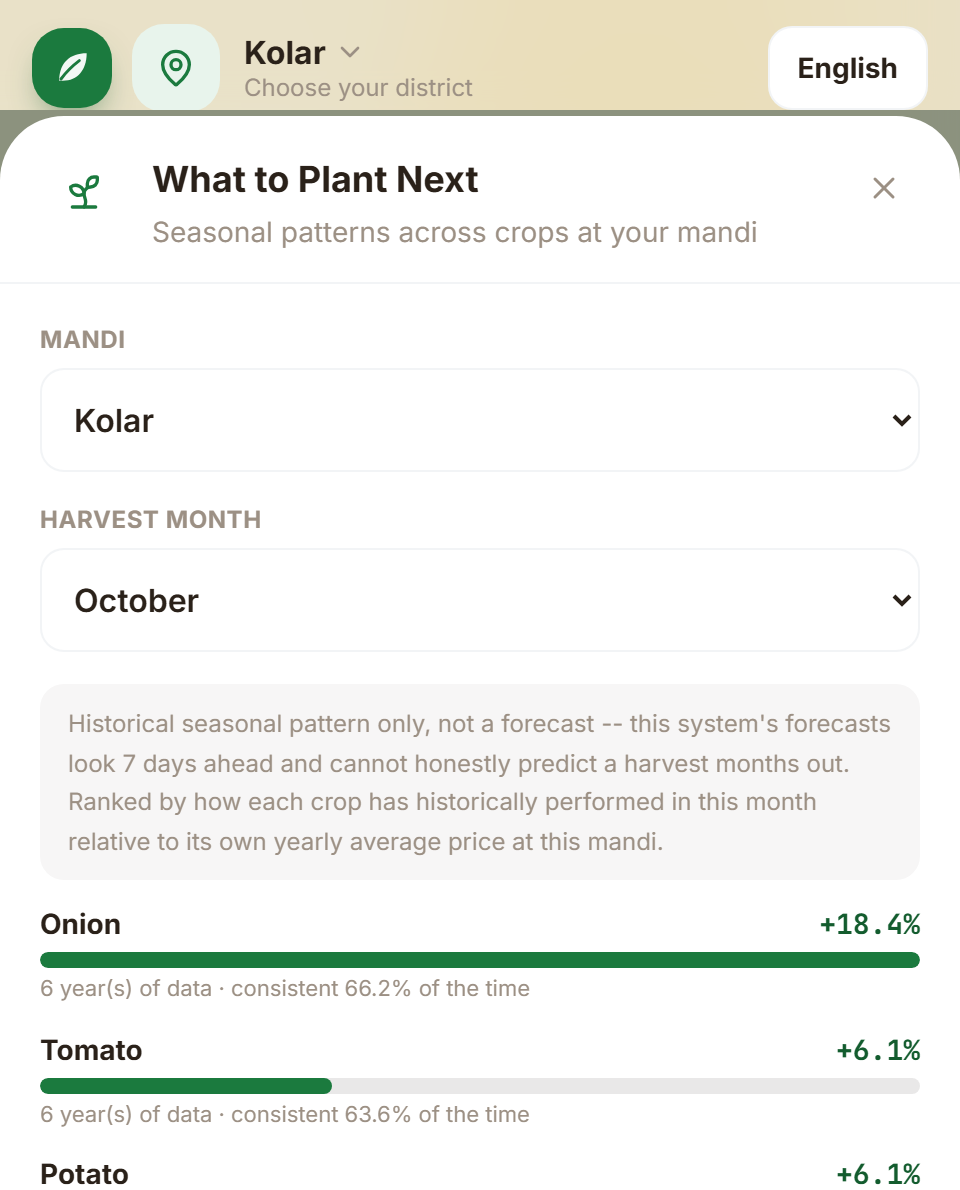
\includegraphics[width=0.94\linewidth,height=9.0cm,keepaspectratio]{figures/shot_t_plant.png}}\\[1mm]{\footnotesize (a) What to plant next}\end{minipage}\hfill
\begin{minipage}[t]{0.485\textwidth}\centering\fbox{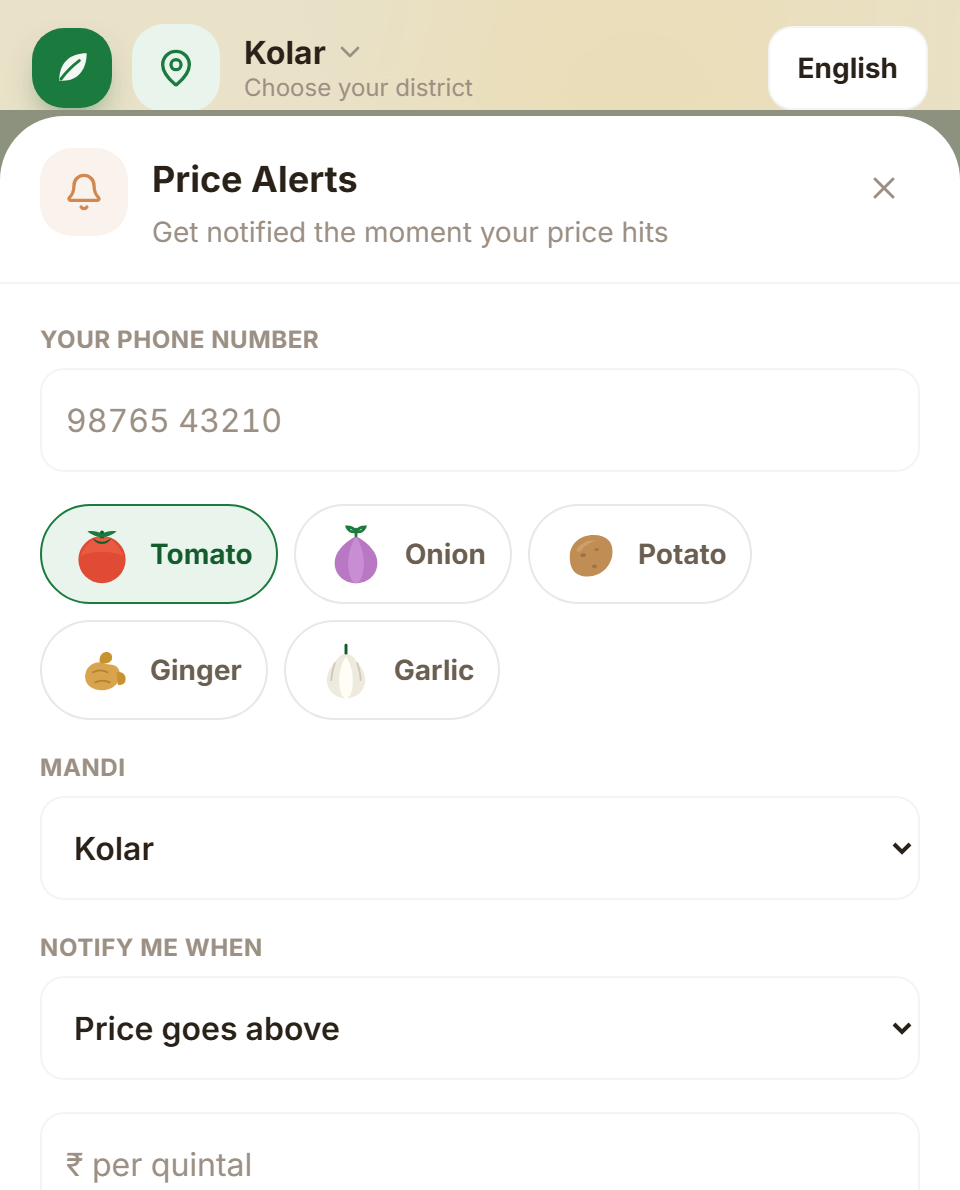
\includegraphics[width=0.94\linewidth,height=9.0cm,keepaspectratio]{figures/shot_t_alerts.png}}\\[1mm]{\footnotesize (b) Price alerts}\end{minipage}
\caption{(a) Seasonal patterns by crop for a chosen harvest month, from past years. (b) A price alert that notifies the farmer when a crop reaches a chosen price.}
\label{fig:sc-tools4}
\end{figure}

What to Plant Next (Figure~\ref{fig:sc-tools4}a) is explicitly historical: it shows how each crop has behaved in the chosen month in previous years and does not forecast the coming season. The alert sheet (b) is the entry point for the Telegram digest of Section~\ref{sec:digest-method}.


\subsection{Advice that can be checked}
The three panels of Figure~\ref{fig:ui-insight} (Section~\ref{sec:insight-method}) sit inside the Best Place sheet. They show the arithmetic behind the choice, what changes if the farmer's costs differ, and how the advice would have done on days it had not seen. The morning digest of Section~\ref{sec:digest-method} is the same advice delivered as a message.

\subsection{Trader desk}
The trader desk is a set of analytical tools for buyers and for the project's own examination of its method. It is laid out for a wide screen.

\begin{figure}[!t]
\centering
\fbox{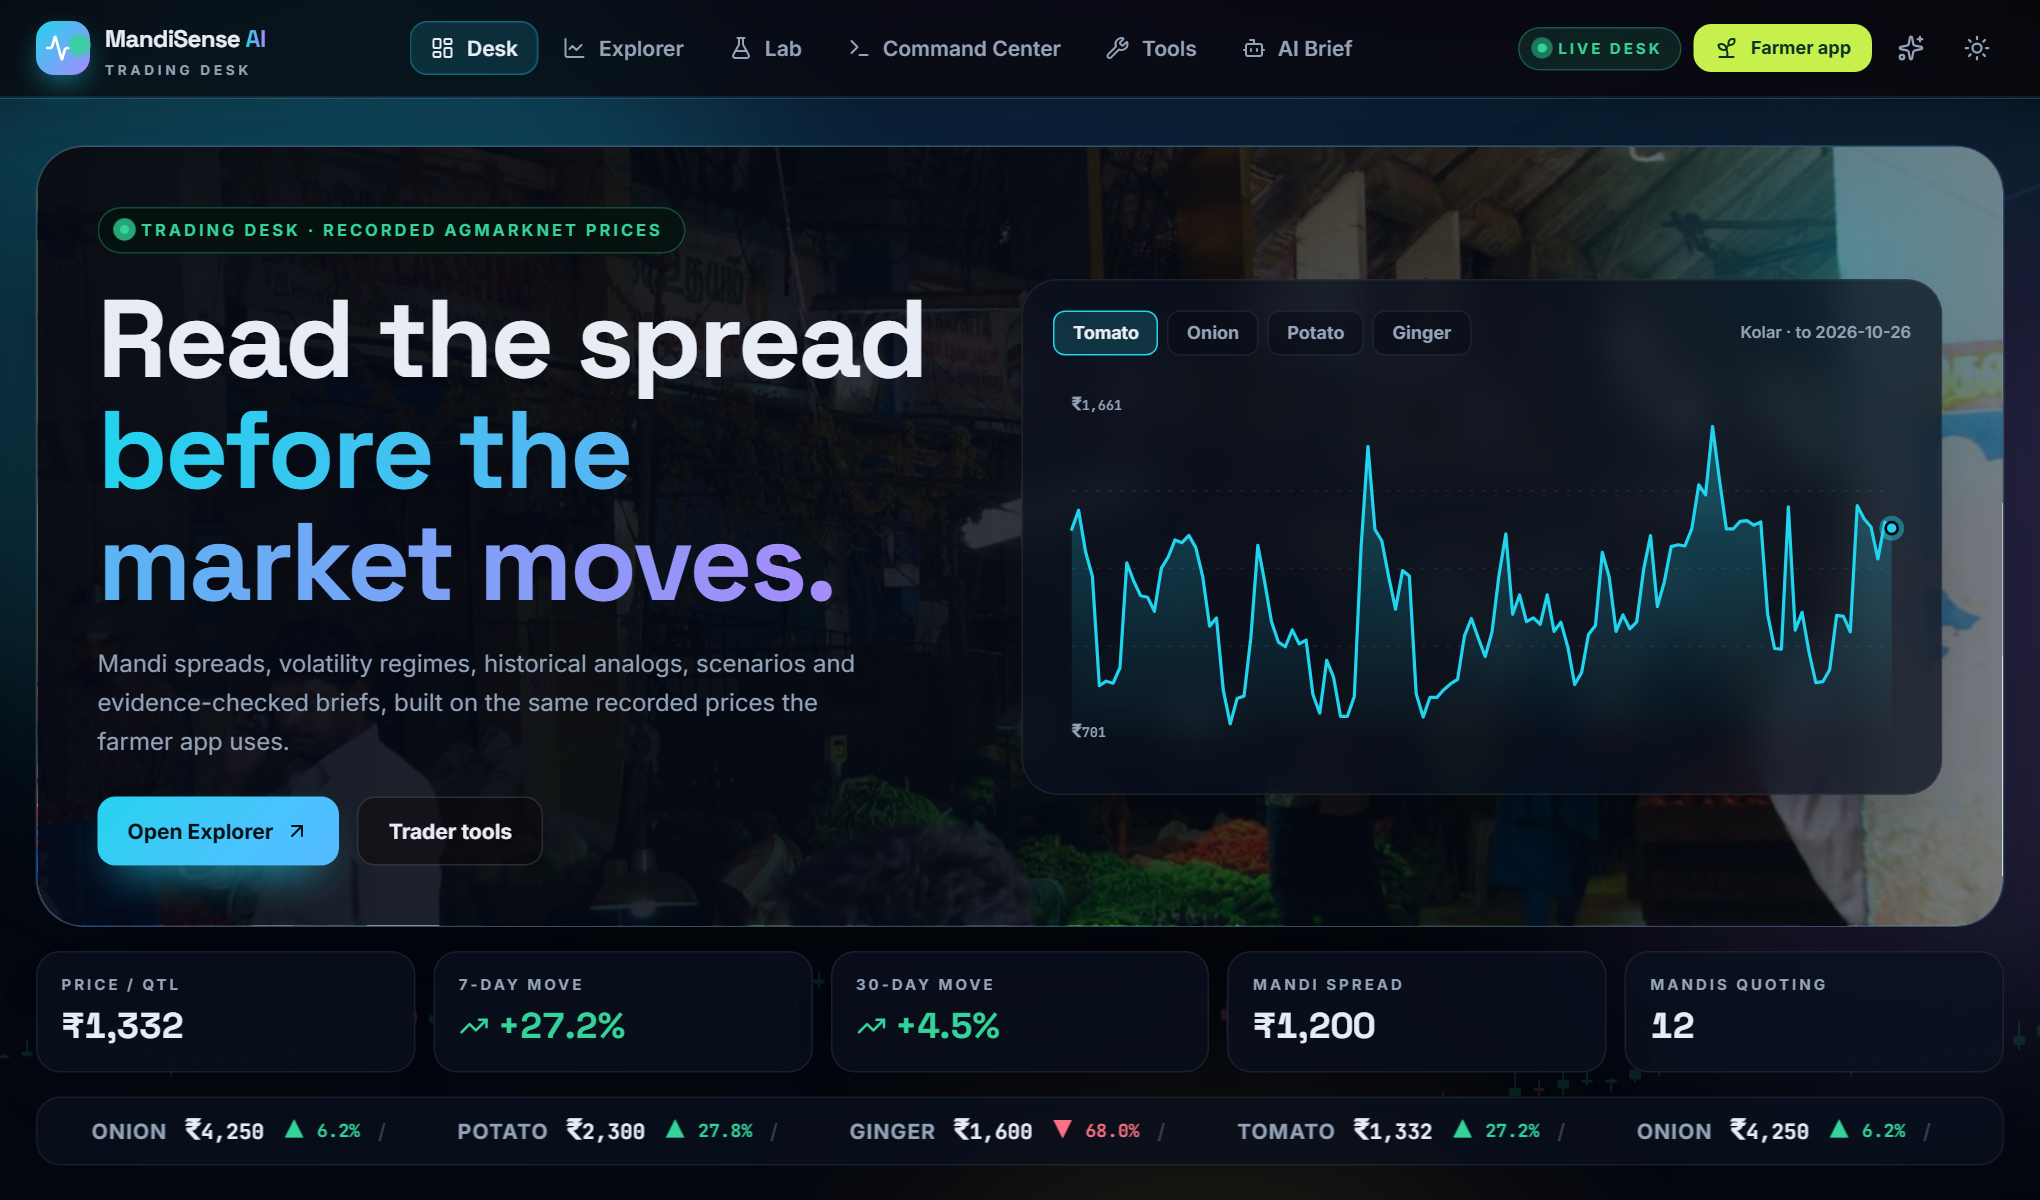
\includegraphics[width=0.93\linewidth]{figures/shot_w_trader.png}}\\[0.5mm]{\footnotesize (a) Trader home: the day's key signals and entry points to the tools below}
\medskip
\fbox{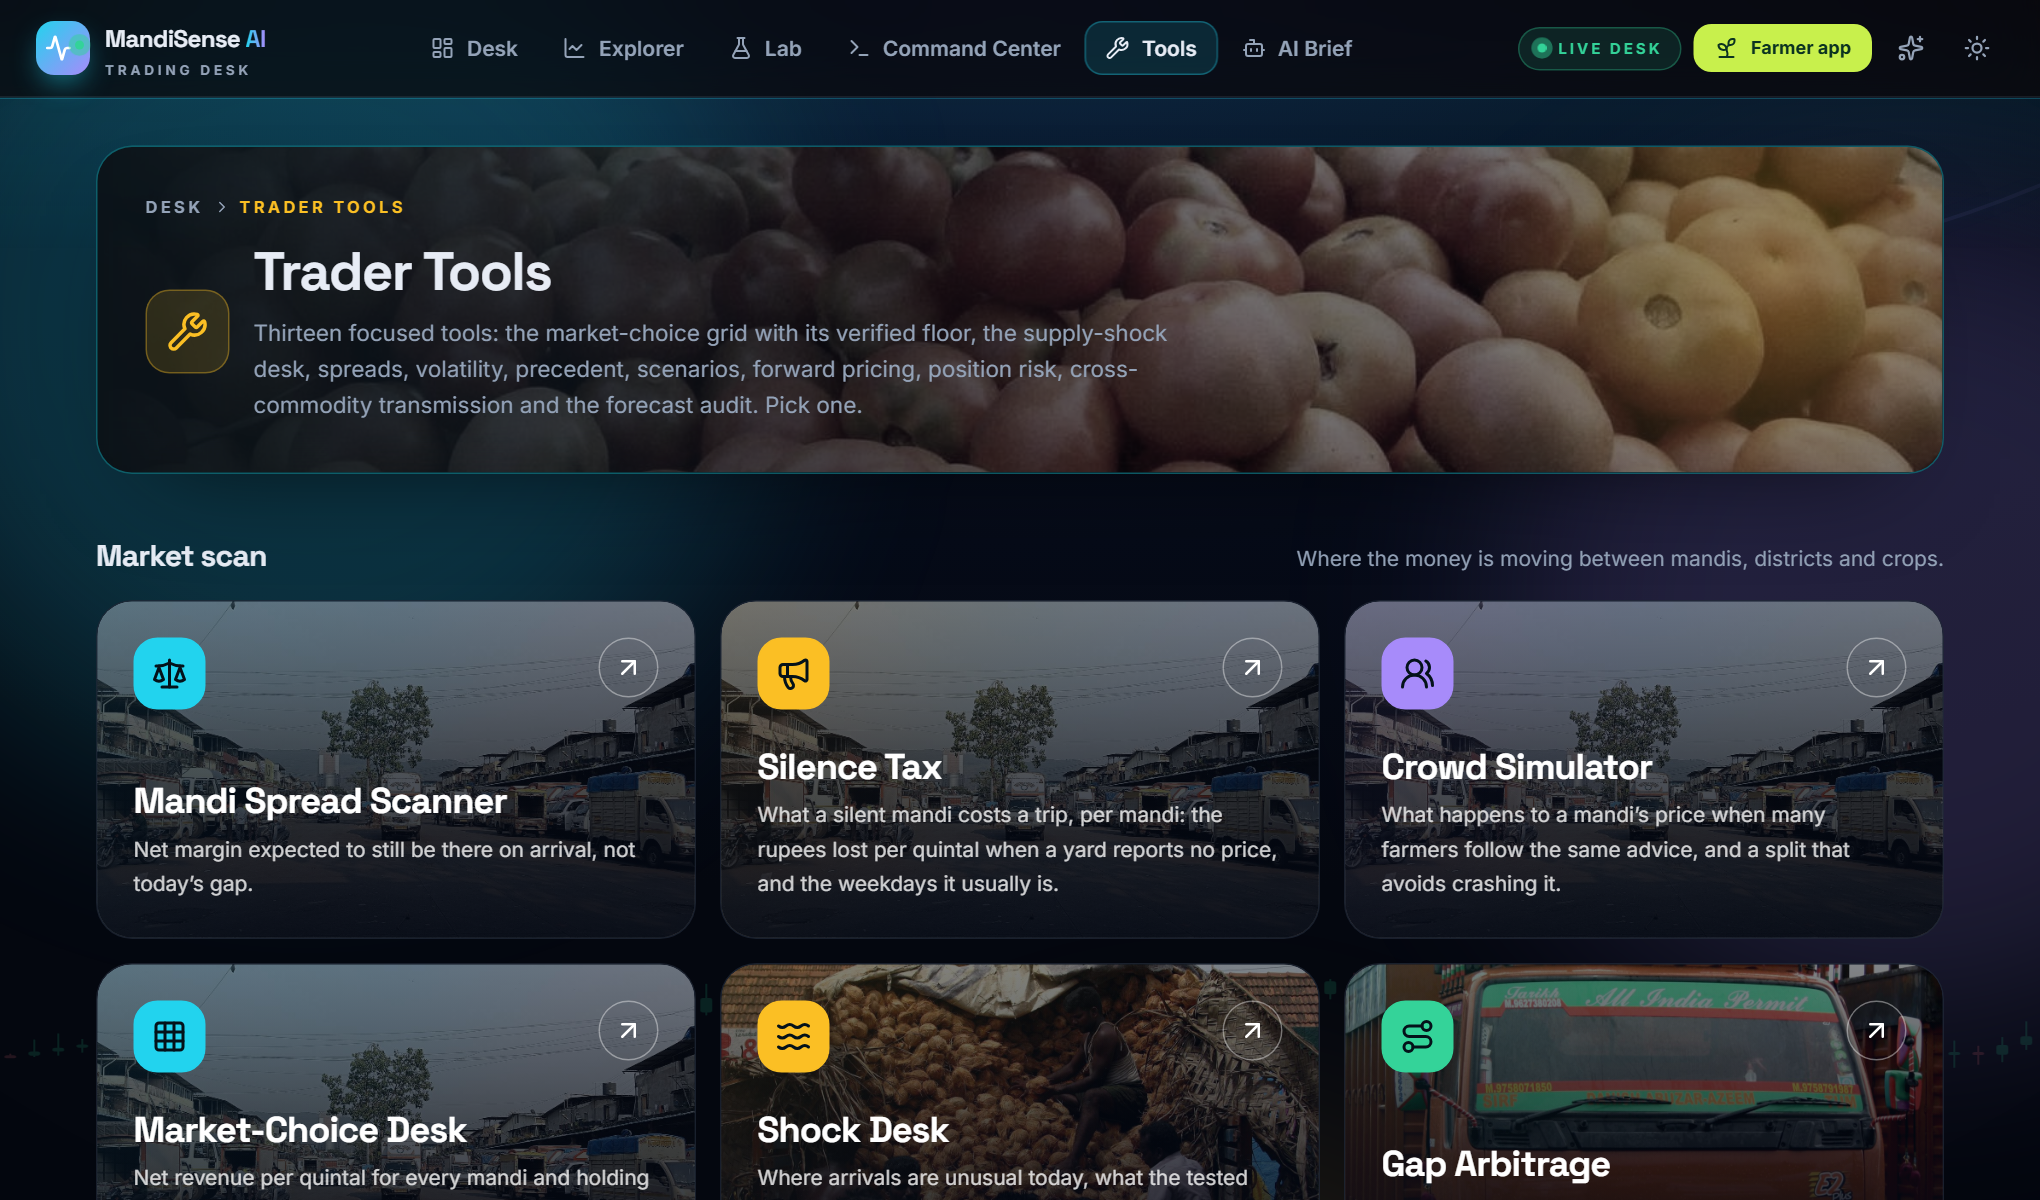
\includegraphics[width=0.93\linewidth]{figures/shot_w_tradertools.png}}\\[0.5mm]{\footnotesize (b) The trader tools index}
\caption{(a) Trader home: the day's key signals and entry points to the tools below. (b) The trader tools index.}
\label{fig:sc-w-trader}
\end{figure}

The trader home page gathers the day's signals, such as the largest price gaps between markets, supply shocks and the status of the advice, and links each to its tool.

The index lists every analytical tool with a one-line statement of the question it answers.

\begin{figure}[!t]
\centering
\fbox{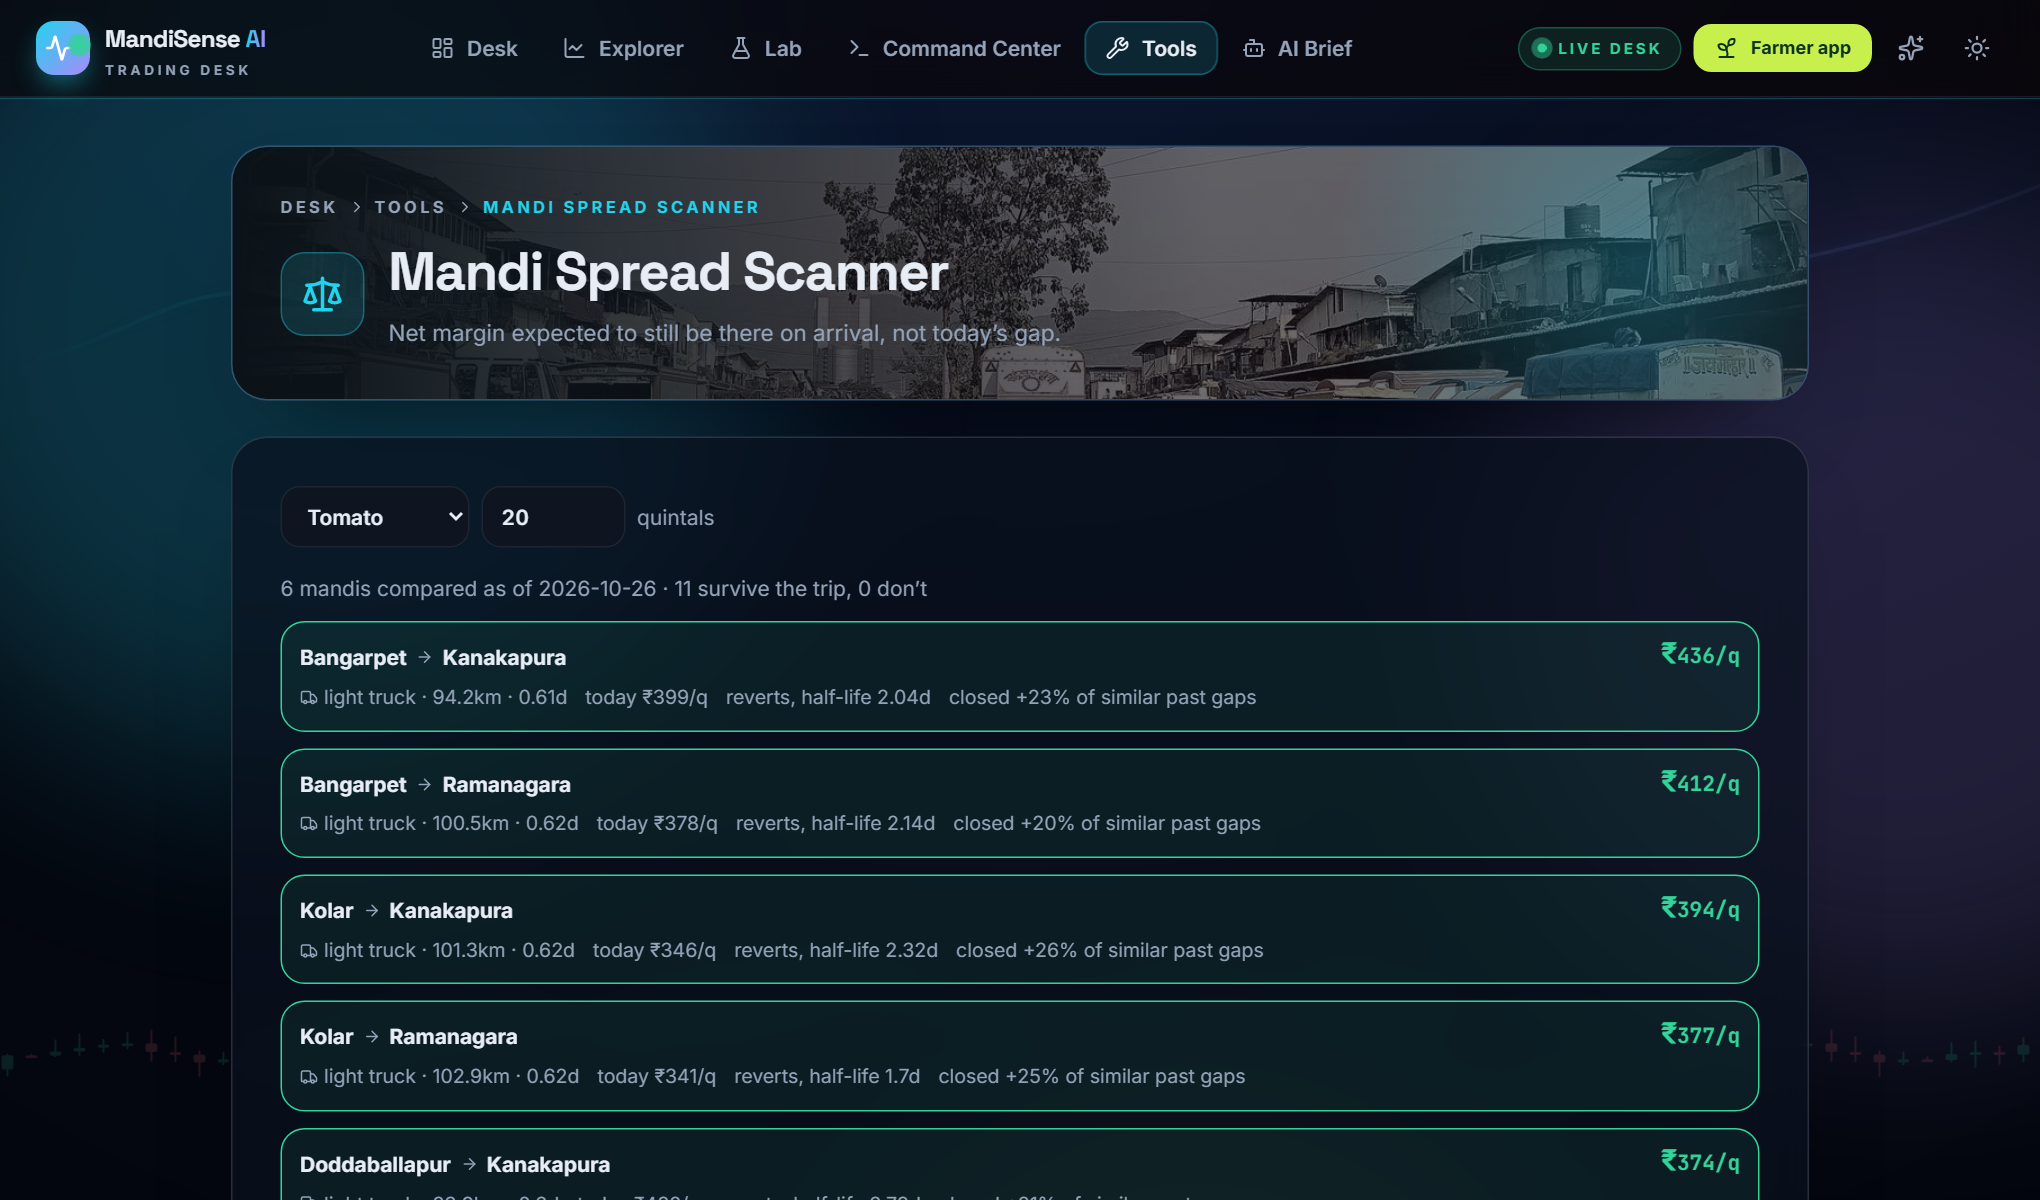
\includegraphics[width=0.93\linewidth]{figures/shot_w_spreads.png}}\\[0.5mm]{\footnotesize (a) Spreads between markets for one commodity}
\medskip
\fbox{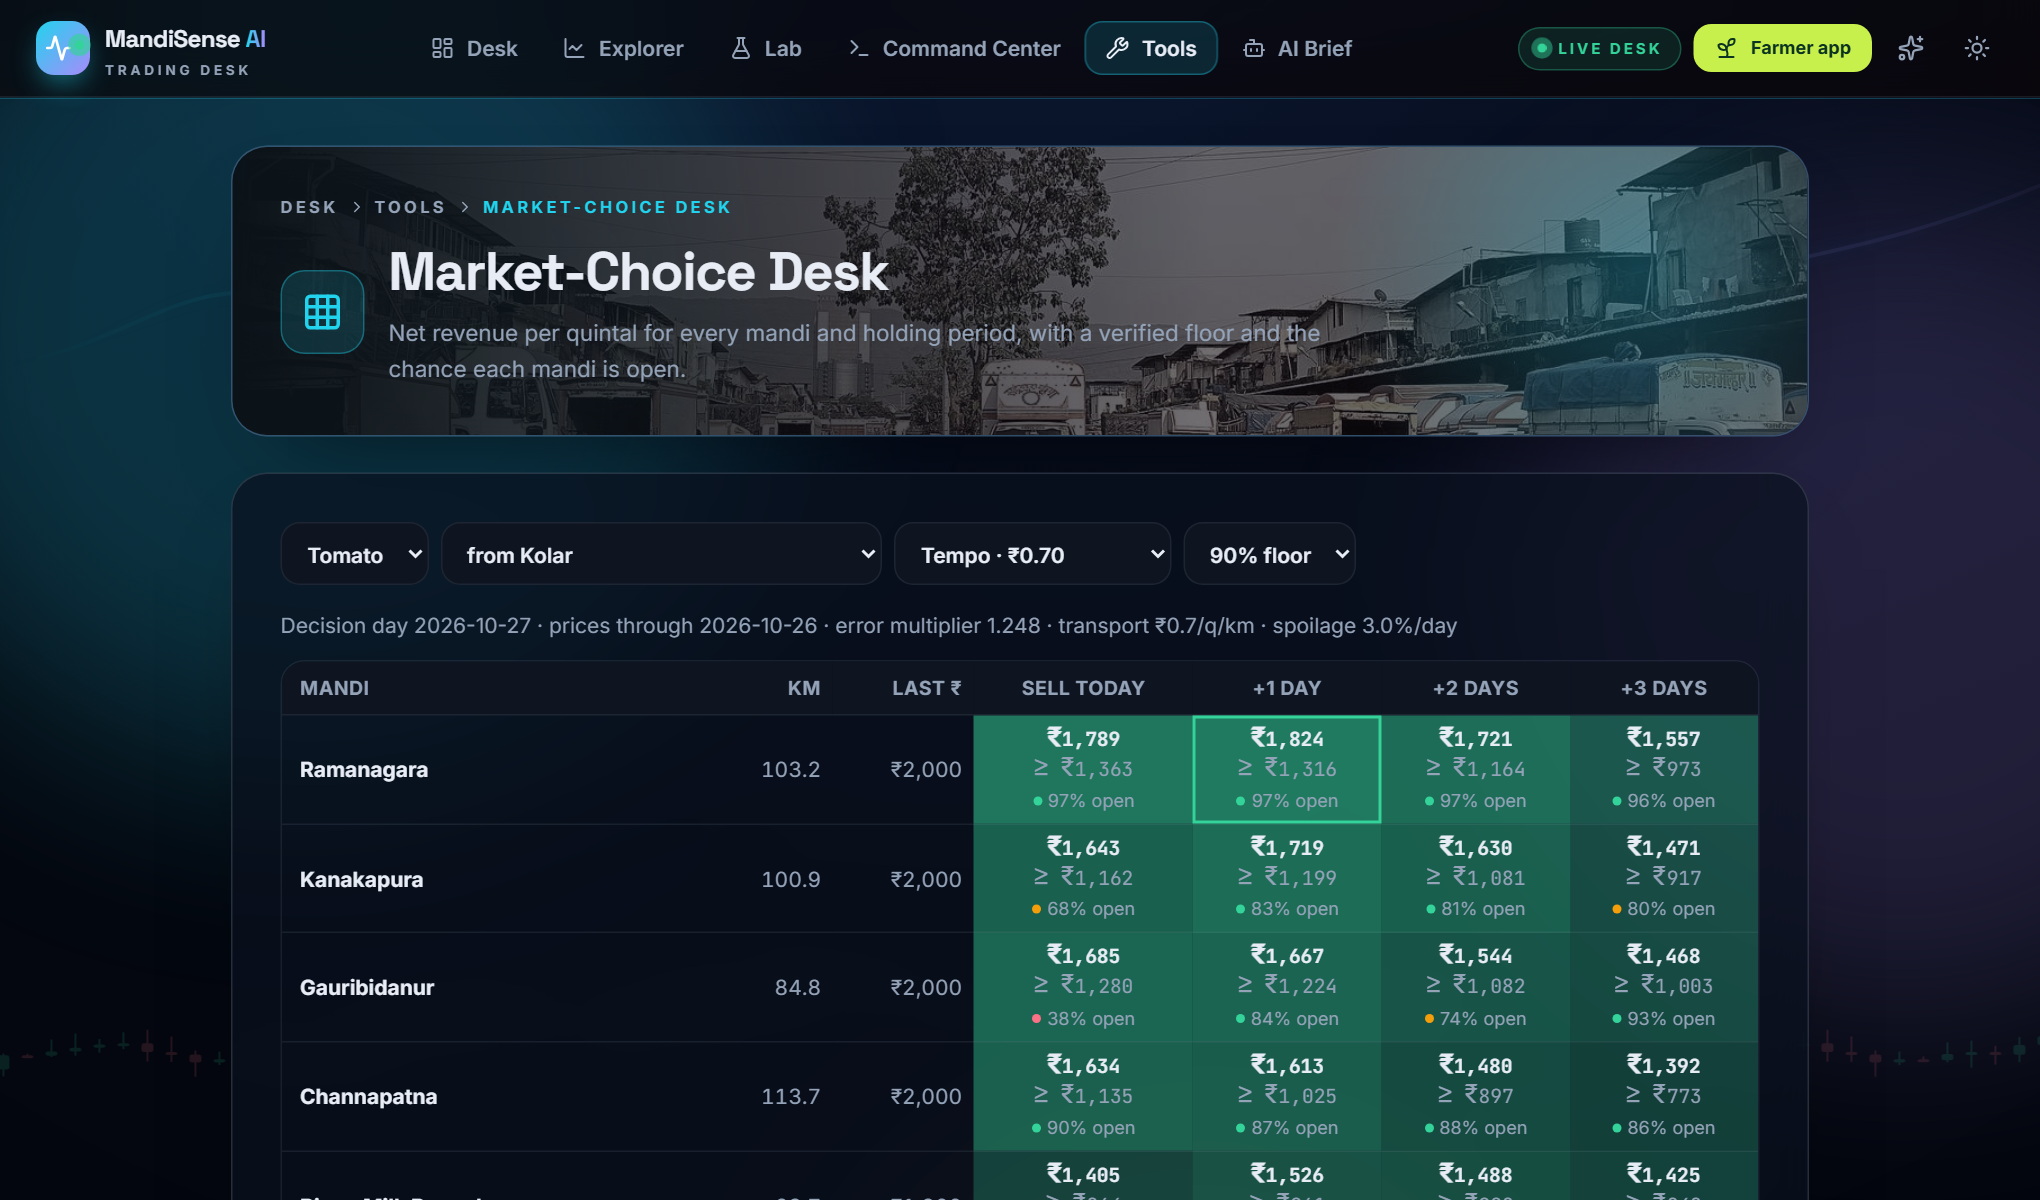
\includegraphics[width=0.93\linewidth]{figures/shot_w_mcdesk.png}}\\[0.5mm]{\footnotesize (b) The market-choice desk: the model's recommended market per day and the revenue floor}
\caption{(a) Spreads between markets for one commodity. (b) The market-choice desk: the model's recommended market per day and the revenue floor.}
\label{fig:sc-w-spreads}
\end{figure}

The spread tool shows the price gap between pairs of markets after transport, with the number of days each gap has lasted. A gap that persists is a signal of a market that is slow to clear.

This is the technical view of the recommendation of Section~\ref{sec:floors}: the chosen market, the expected and floor revenue, the alternatives and the model that produced them.

\begin{figure}[!t]
\centering
\fbox{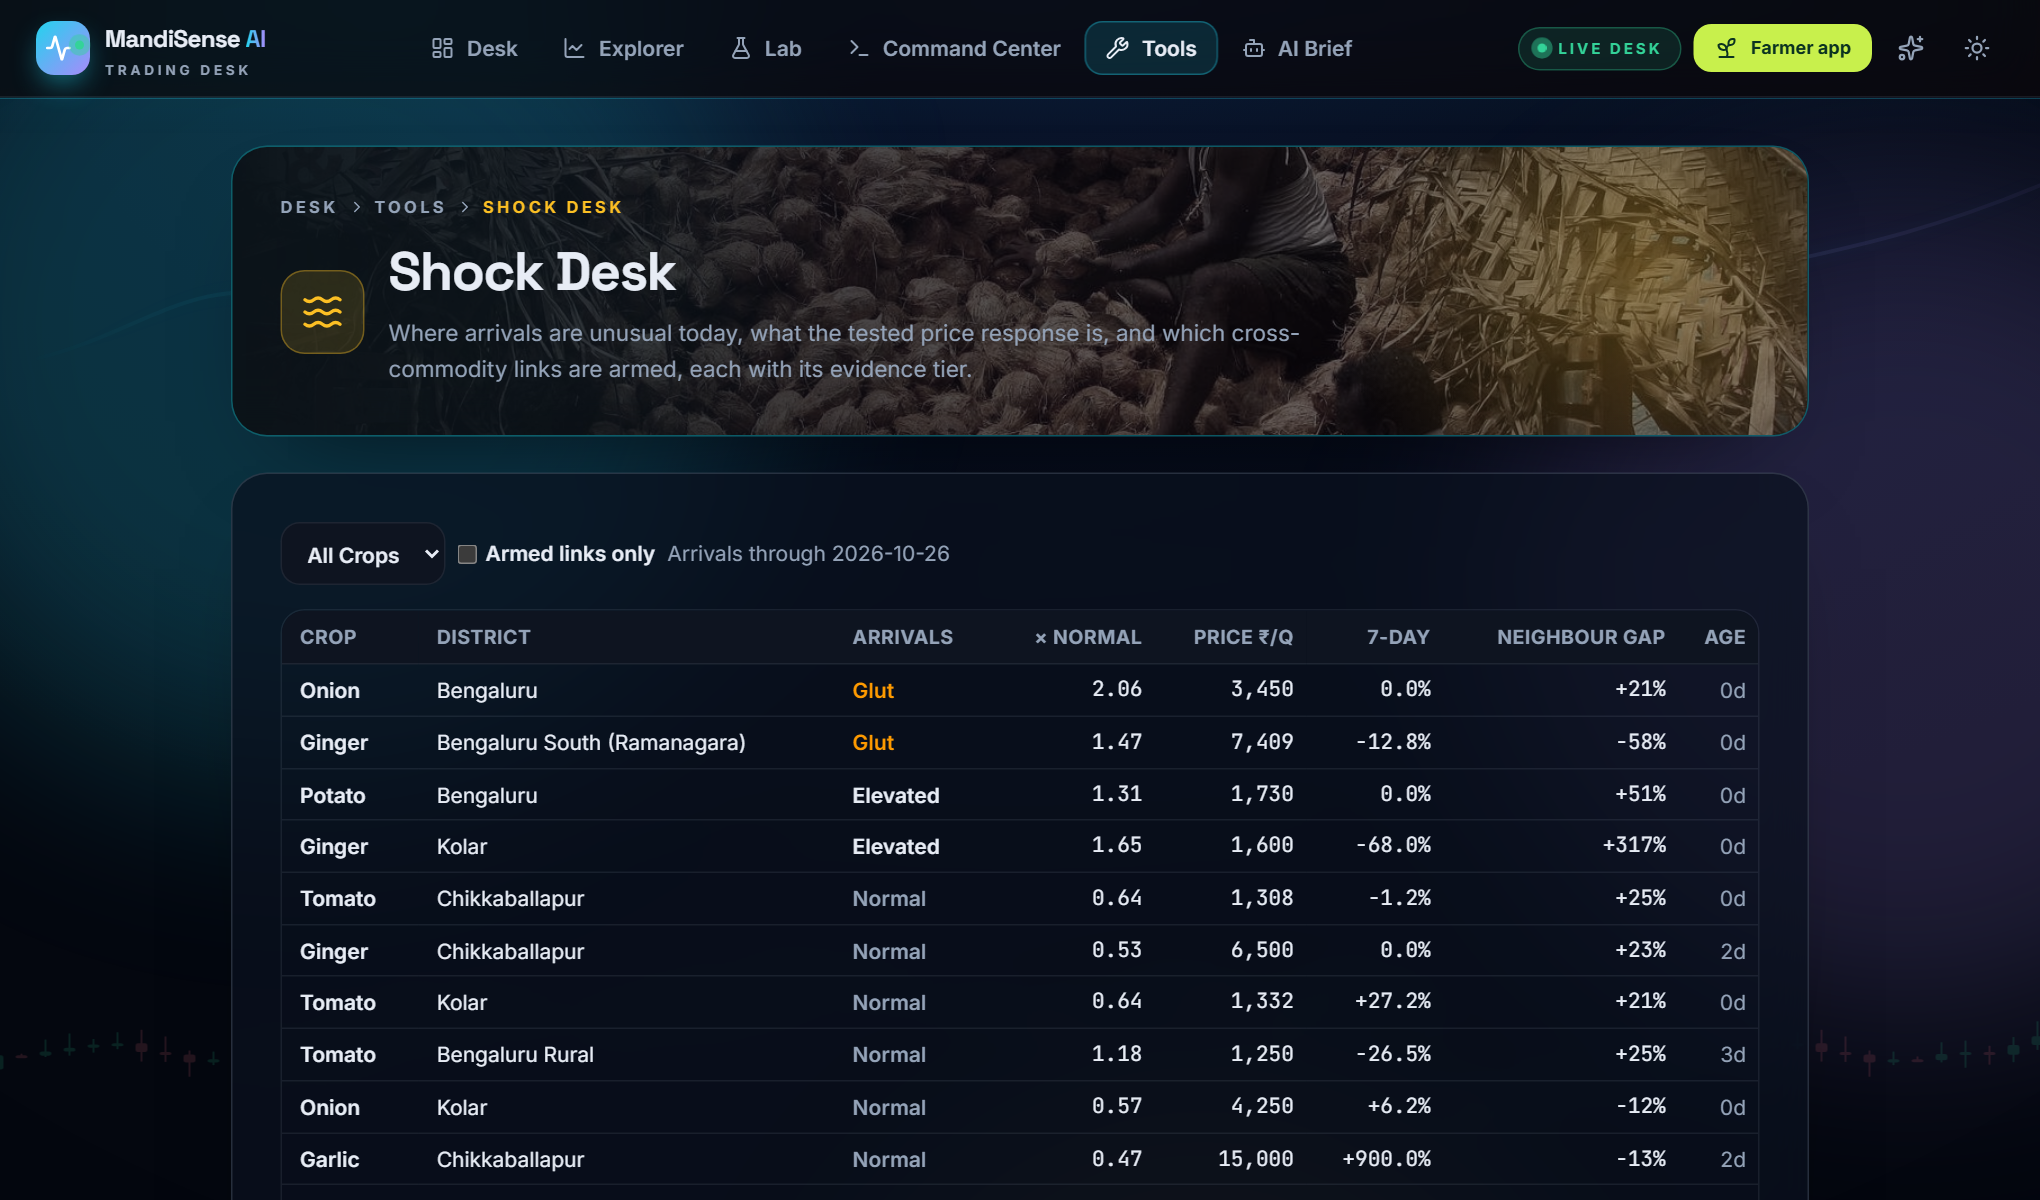
\includegraphics[width=0.93\linewidth]{figures/shot_w_shock.png}}\\[0.5mm]{\footnotesize (a) The shock desk: unusual price moves, with the markets affected}
\medskip
\fbox{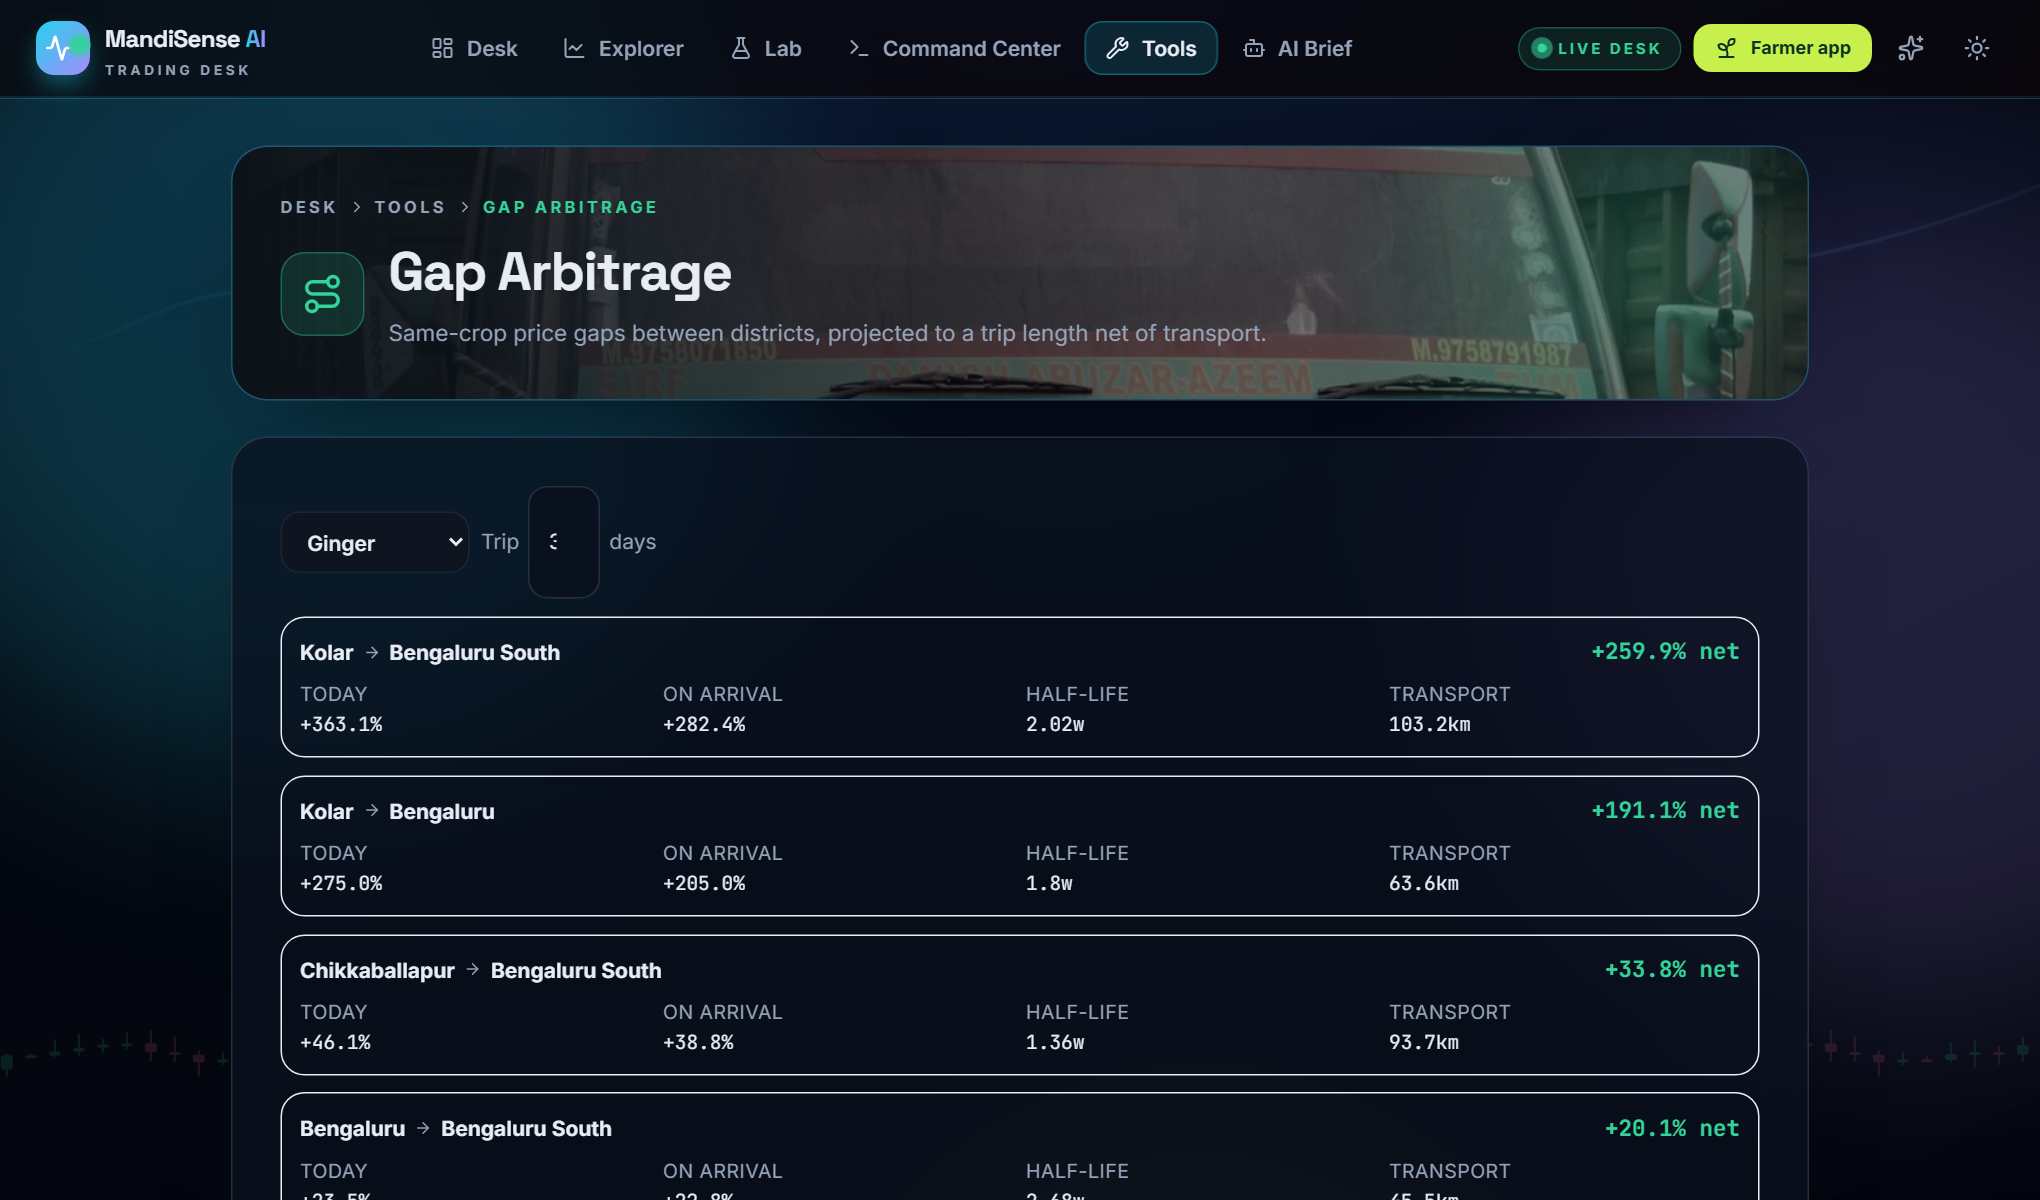
\includegraphics[width=0.93\linewidth]{figures/shot_w_gap.png}}\\[0.5mm]{\footnotesize (b) Gap arbitrage between mandis}
\caption{(a) The shock desk: unusual price moves, with the markets affected. (b) Gap arbitrage between mandis.}
\label{fig:sc-w-shock}
\end{figure}

The desk lists price moves that are unusual relative to a rolling baseline and the markets where they appear. It feeds the shock episodes used for the transmission test of Section~\ref{sec:spill-method}.

The tool pairs a high-price and a low-price market, deducts transport and shrinkage, and shows whether a gap is worth acting on.

\begin{figure}[!t]
\centering
\fbox{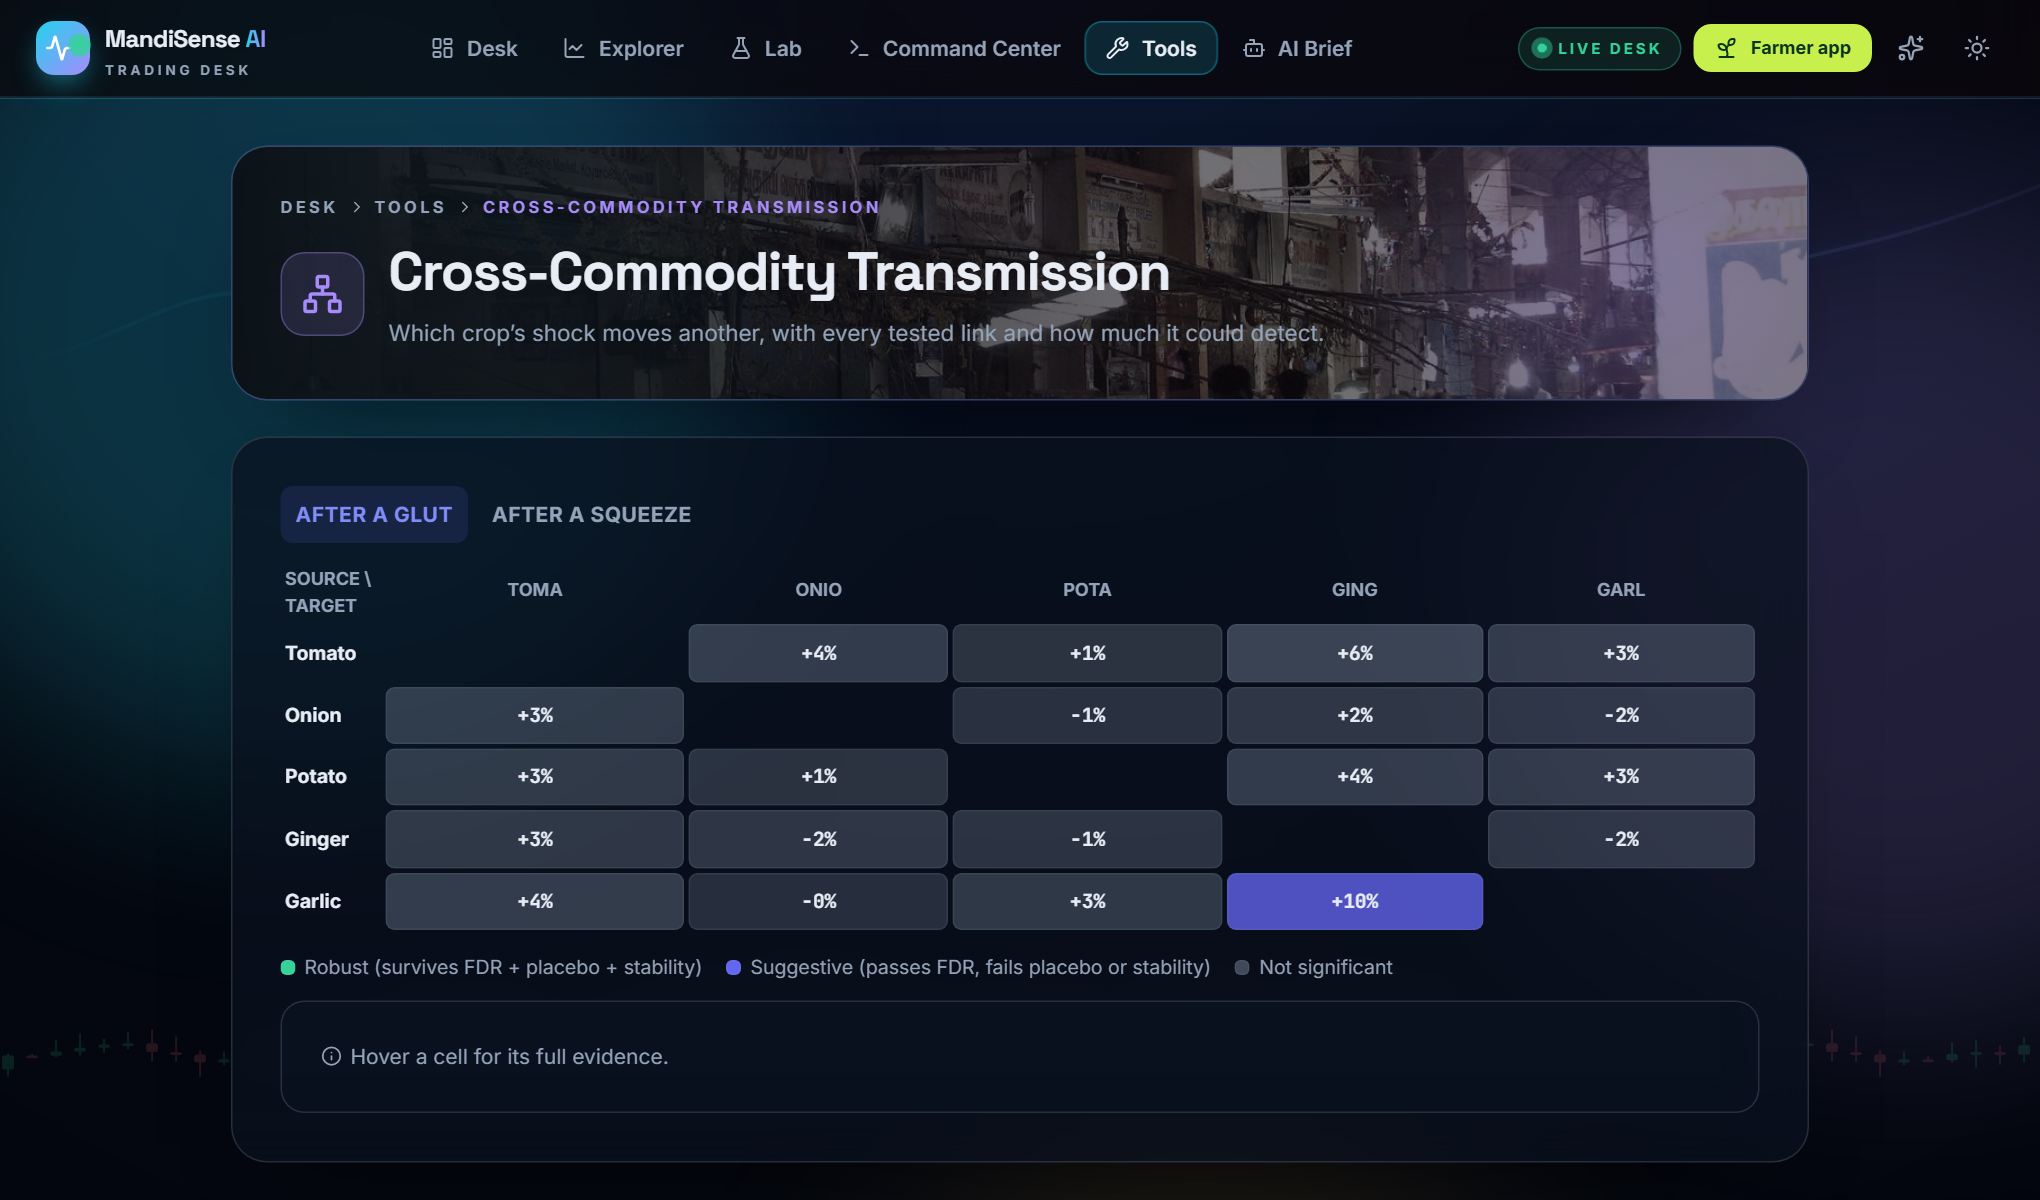
\includegraphics[width=0.93\linewidth]{figures/shot_w_transmission.png}}\\[0.5mm]{\footnotesize (a) Cross-commodity transmission}
\medskip
\fbox{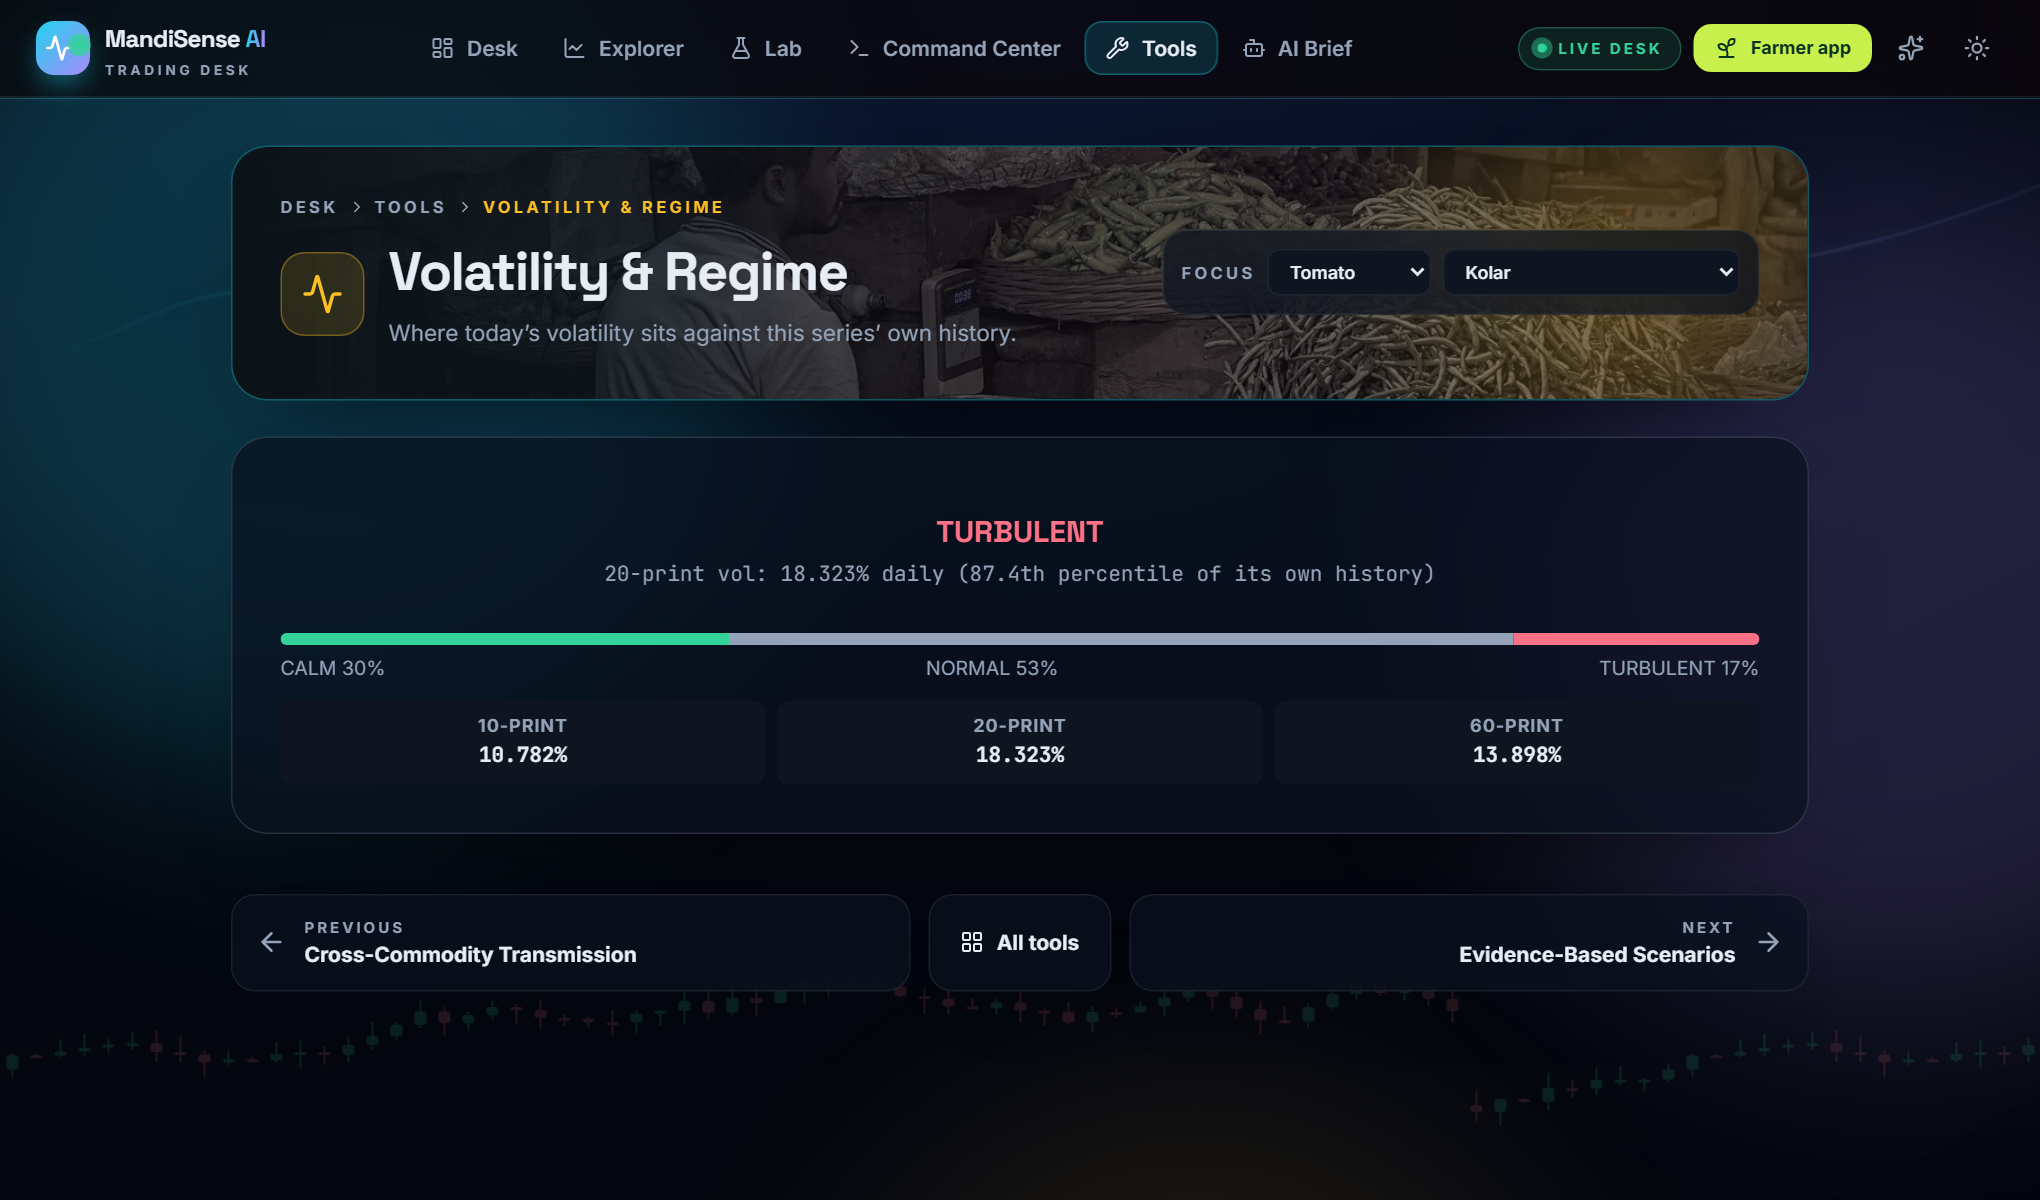
\includegraphics[width=0.93\linewidth]{figures/shot_w_volatility.png}}\\[0.5mm]{\footnotesize (b) Price volatility by commodity and market}
\caption{(a) Cross-commodity transmission. (b) Price volatility by commodity and market.}
\label{fig:sc-w-transmission}
\end{figure}

The transmission page shows the estimated response of one crop to a shock in another. When the evidence is too thin the page says so and shows no number, which is the withholding behaviour described in Section~\ref{sec:transmission}.

Rolling volatility of each series, which the farmer pages translate into a plain warning when a price is unusually unsettled.

\begin{figure}[!t]
\centering
\fbox{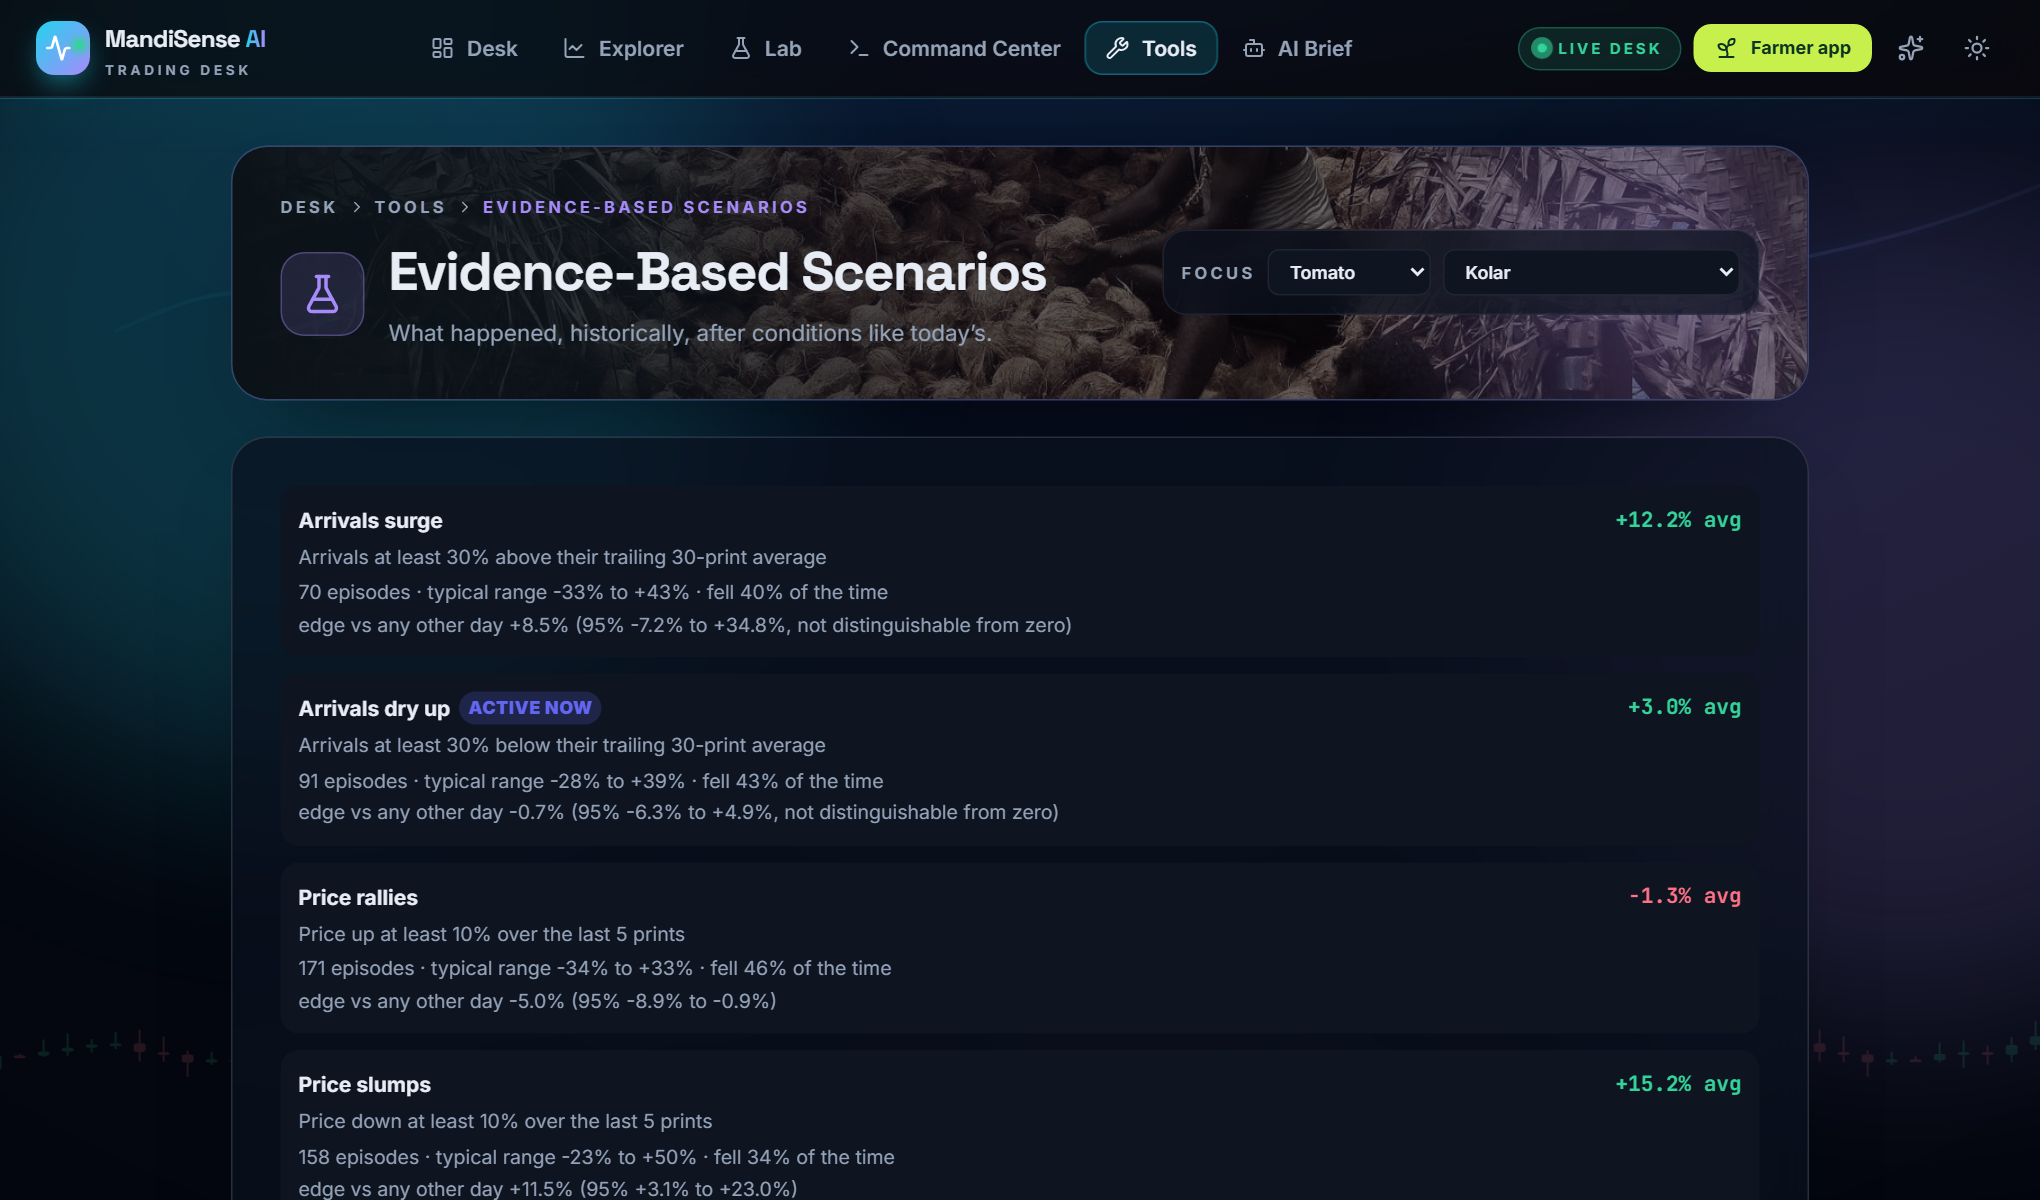
\includegraphics[width=0.93\linewidth]{figures/shot_w_scenarios.png}}\\[0.5mm]{\footnotesize (a) Scenario analysis for the revenue of a sale plan}
\medskip
\fbox{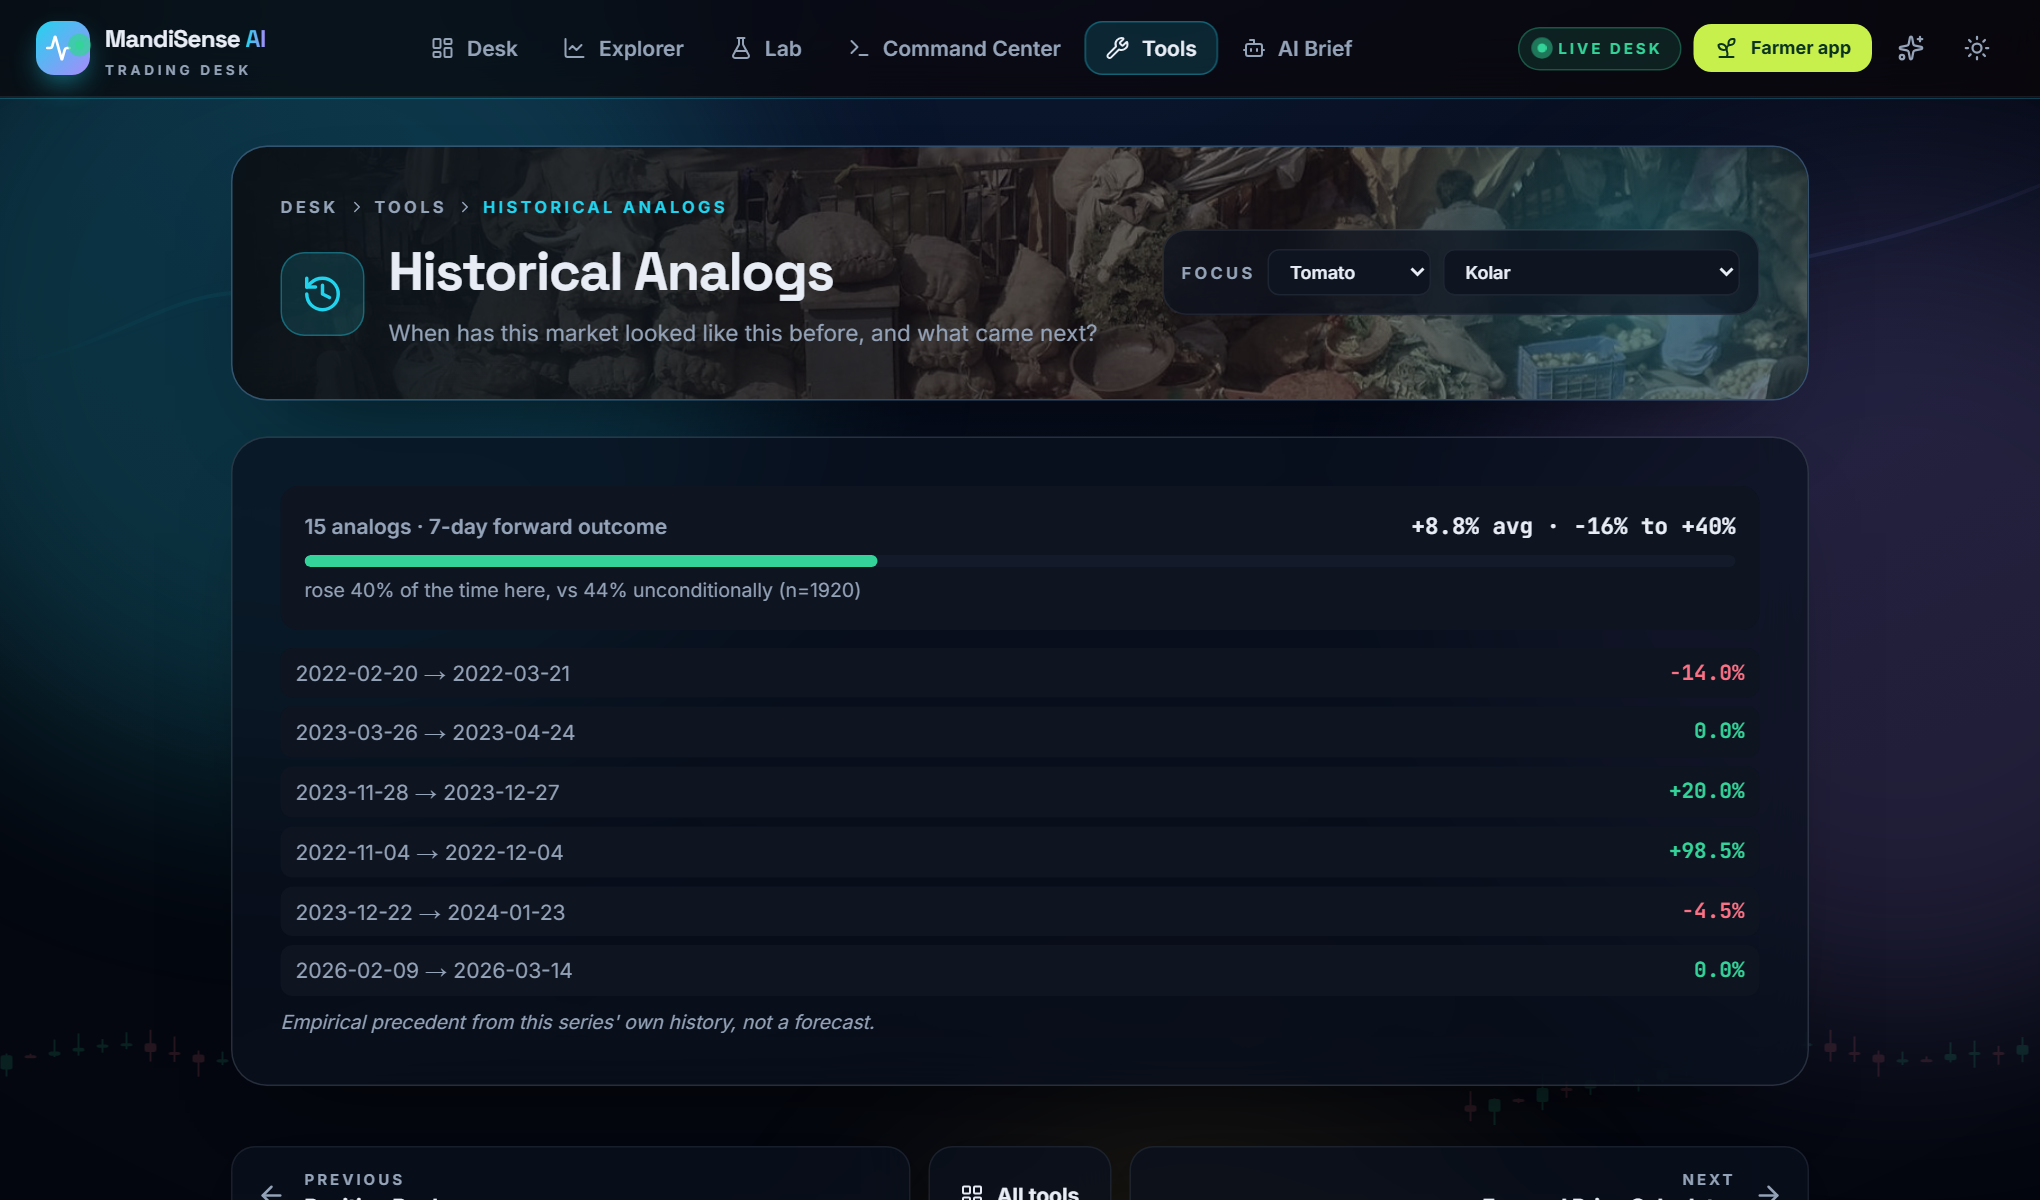
\includegraphics[width=0.93\linewidth]{figures/shot_w_analogs.png}}\\[0.5mm]{\footnotesize (b) Analog days: past days that resembled today}
\caption{(a) Scenario analysis for the revenue of a sale plan. (b) Analog days: past days that resembled today.}
\label{fig:sc-w-scenarios}
\end{figure}

The tool changes transport cost, shrinkage and price in turn and shows how the recommended choice and its revenue respond.

The page finds earlier days with a similar price pattern and shows what followed, as an aid to judgement and not as a forecast.

\begin{figure}[!t]
\centering
\fbox{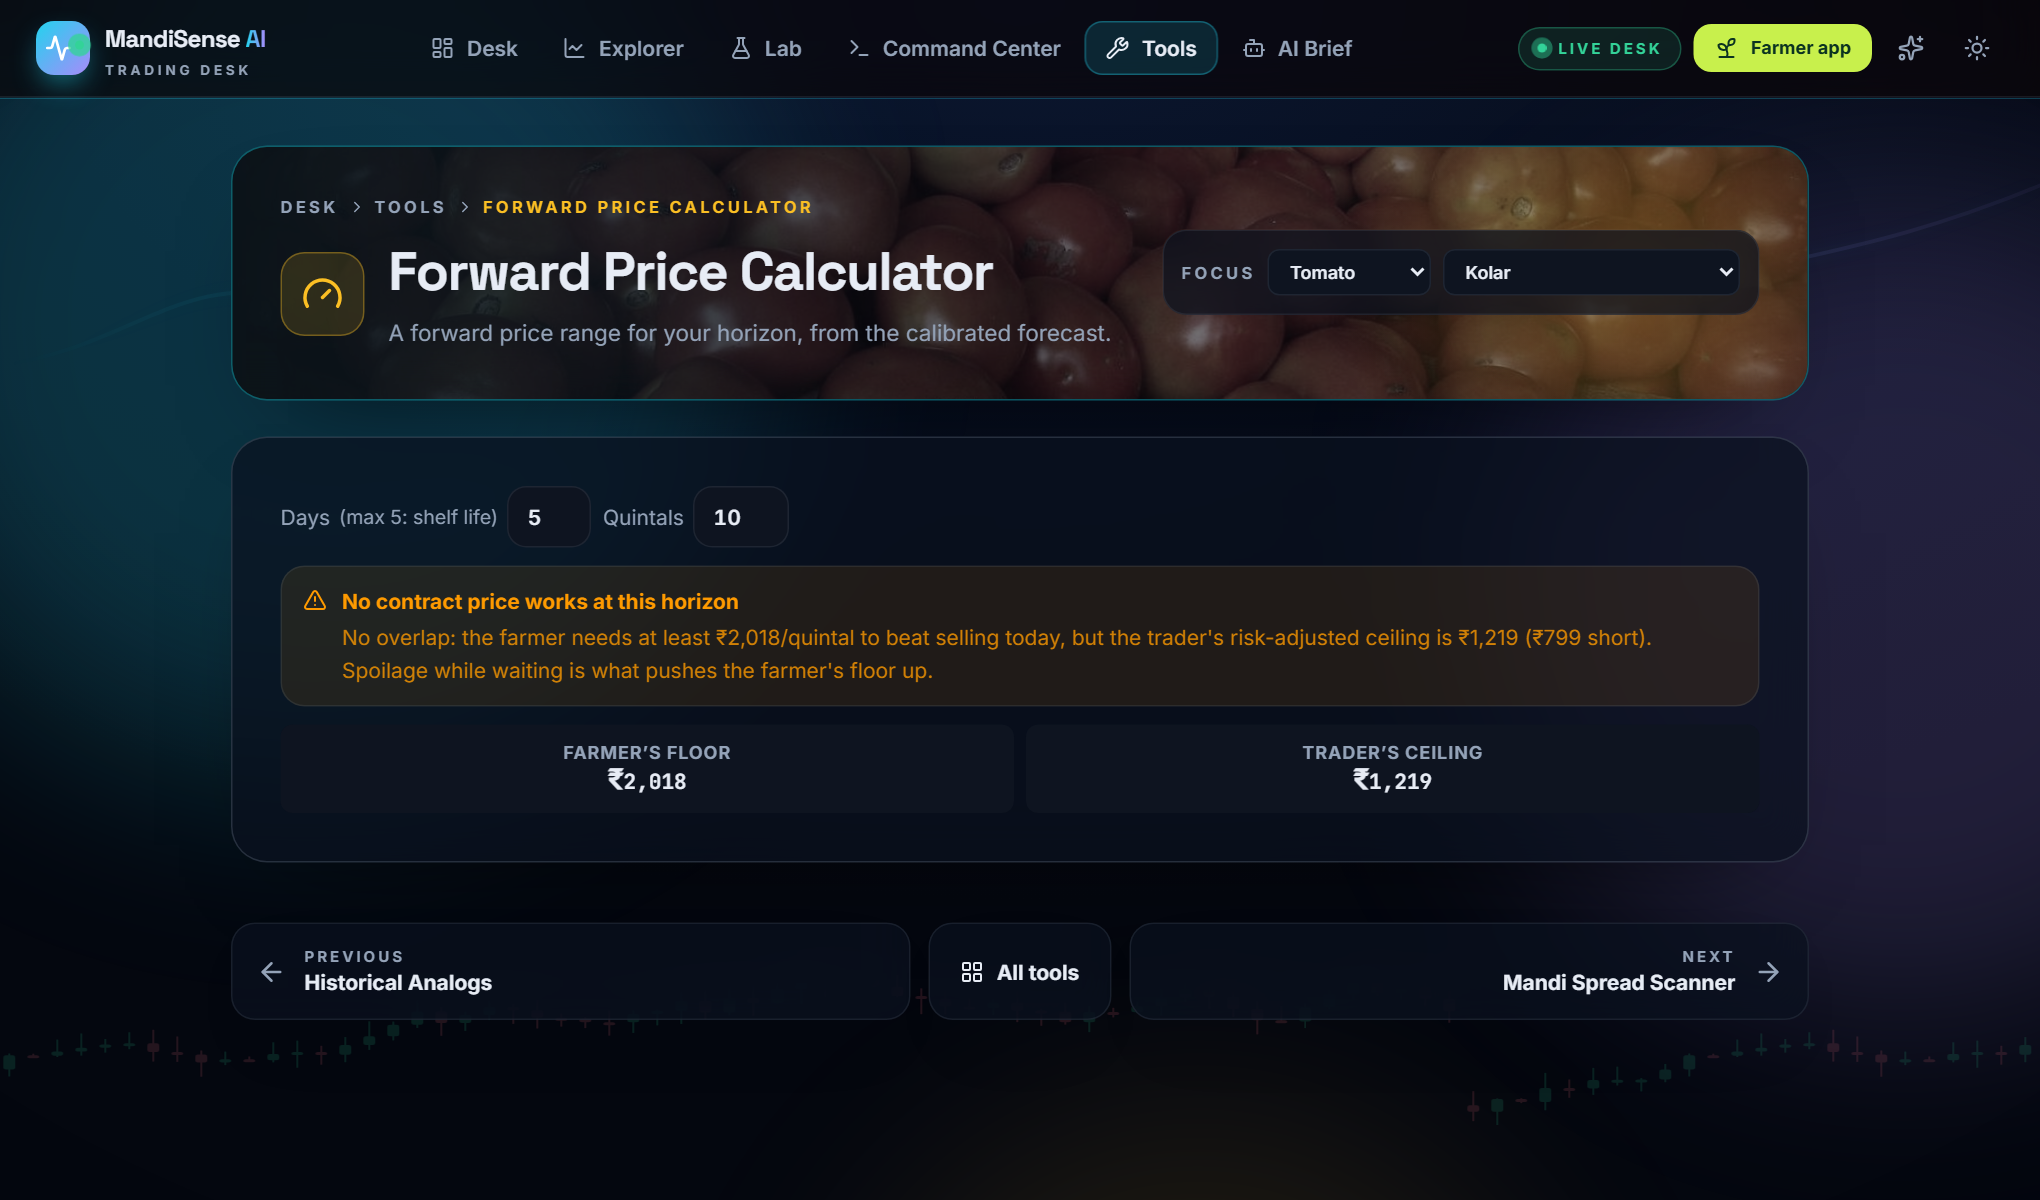
\includegraphics[width=0.93\linewidth]{figures/shot_w_forward.png}}\\[0.5mm]{\footnotesize (a) Forward price view}
\medskip
\fbox{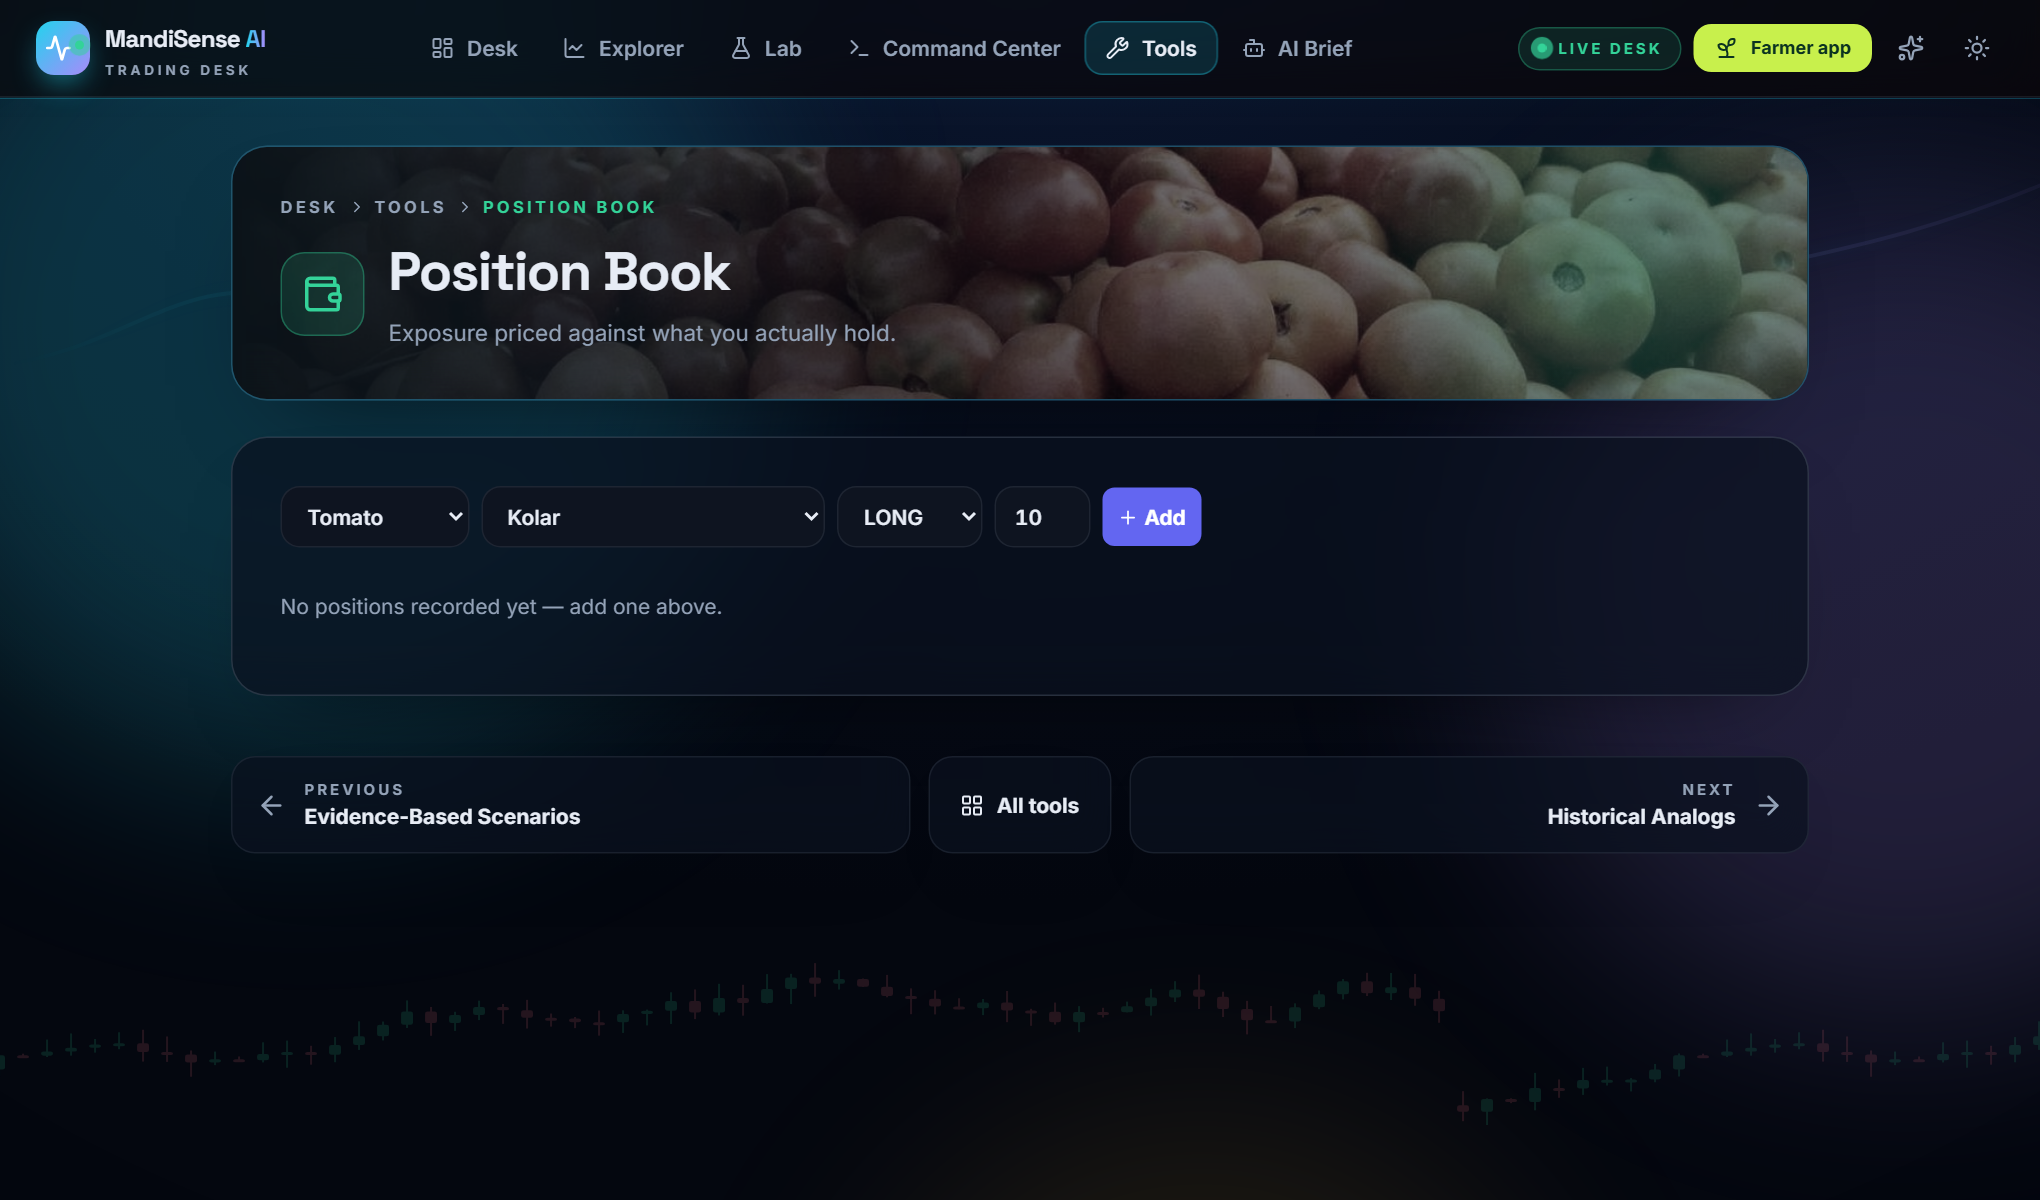
\includegraphics[width=0.93\linewidth]{figures/shot_w_positions.png}}\\[0.5mm]{\footnotesize (b) Positions: the sales a trader is tracking}
\caption{(a) Forward price view. (b) Positions: the sales a trader is tracking.}
\label{fig:sc-w-forward}
\end{figure}

A forecast with its interval for the coming days, with the forecasting model named on the page.

A small ledger of intended sales with their marked-to-market value.

\begin{figure}[!t]
\centering
\fbox{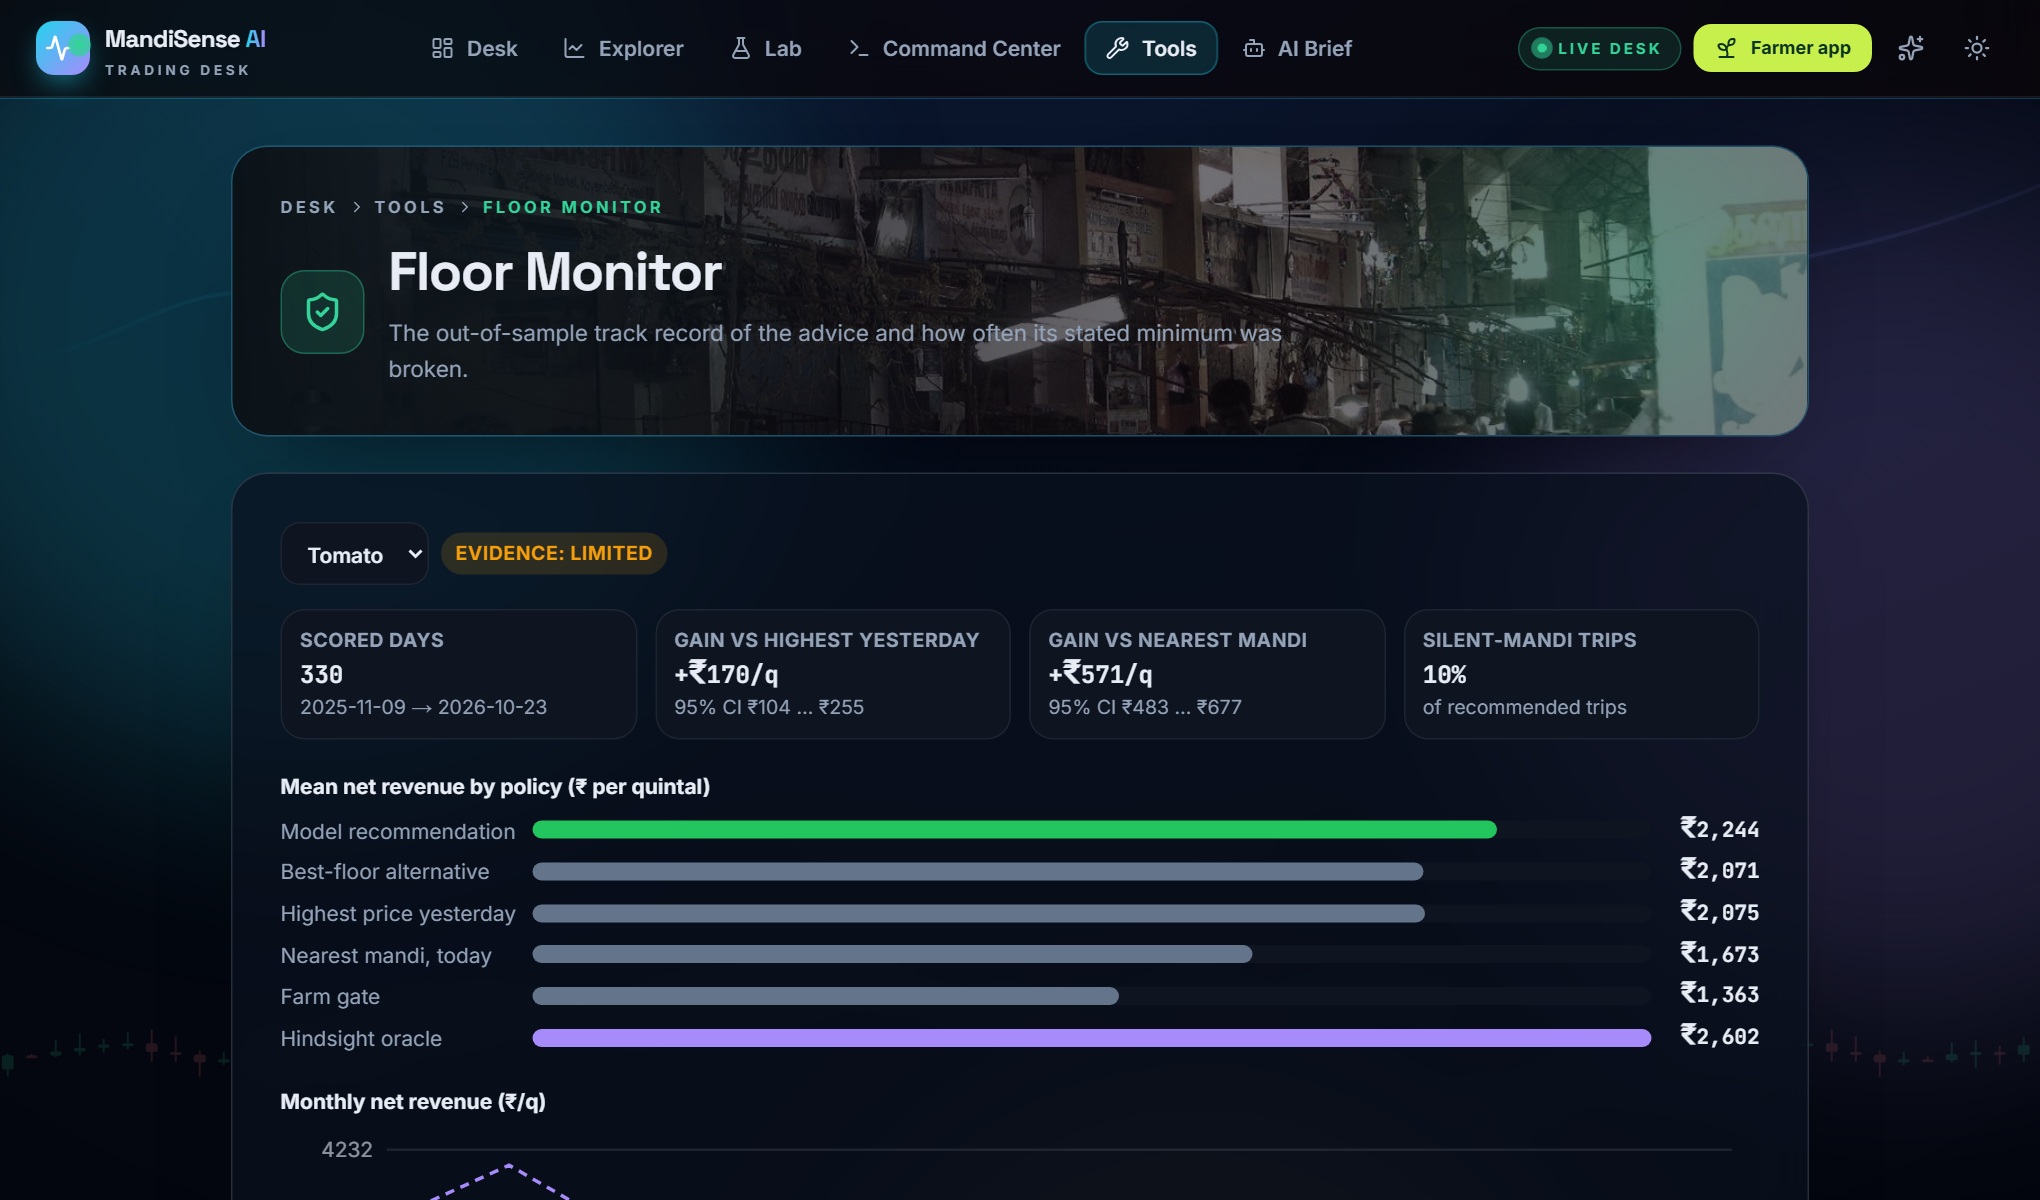
\includegraphics[width=0.93\linewidth]{figures/shot_w_floormon.png}}\\[0.5mm]{\footnotesize (a) Floor monitor: how often the revenue floor has held}
\medskip
\fbox{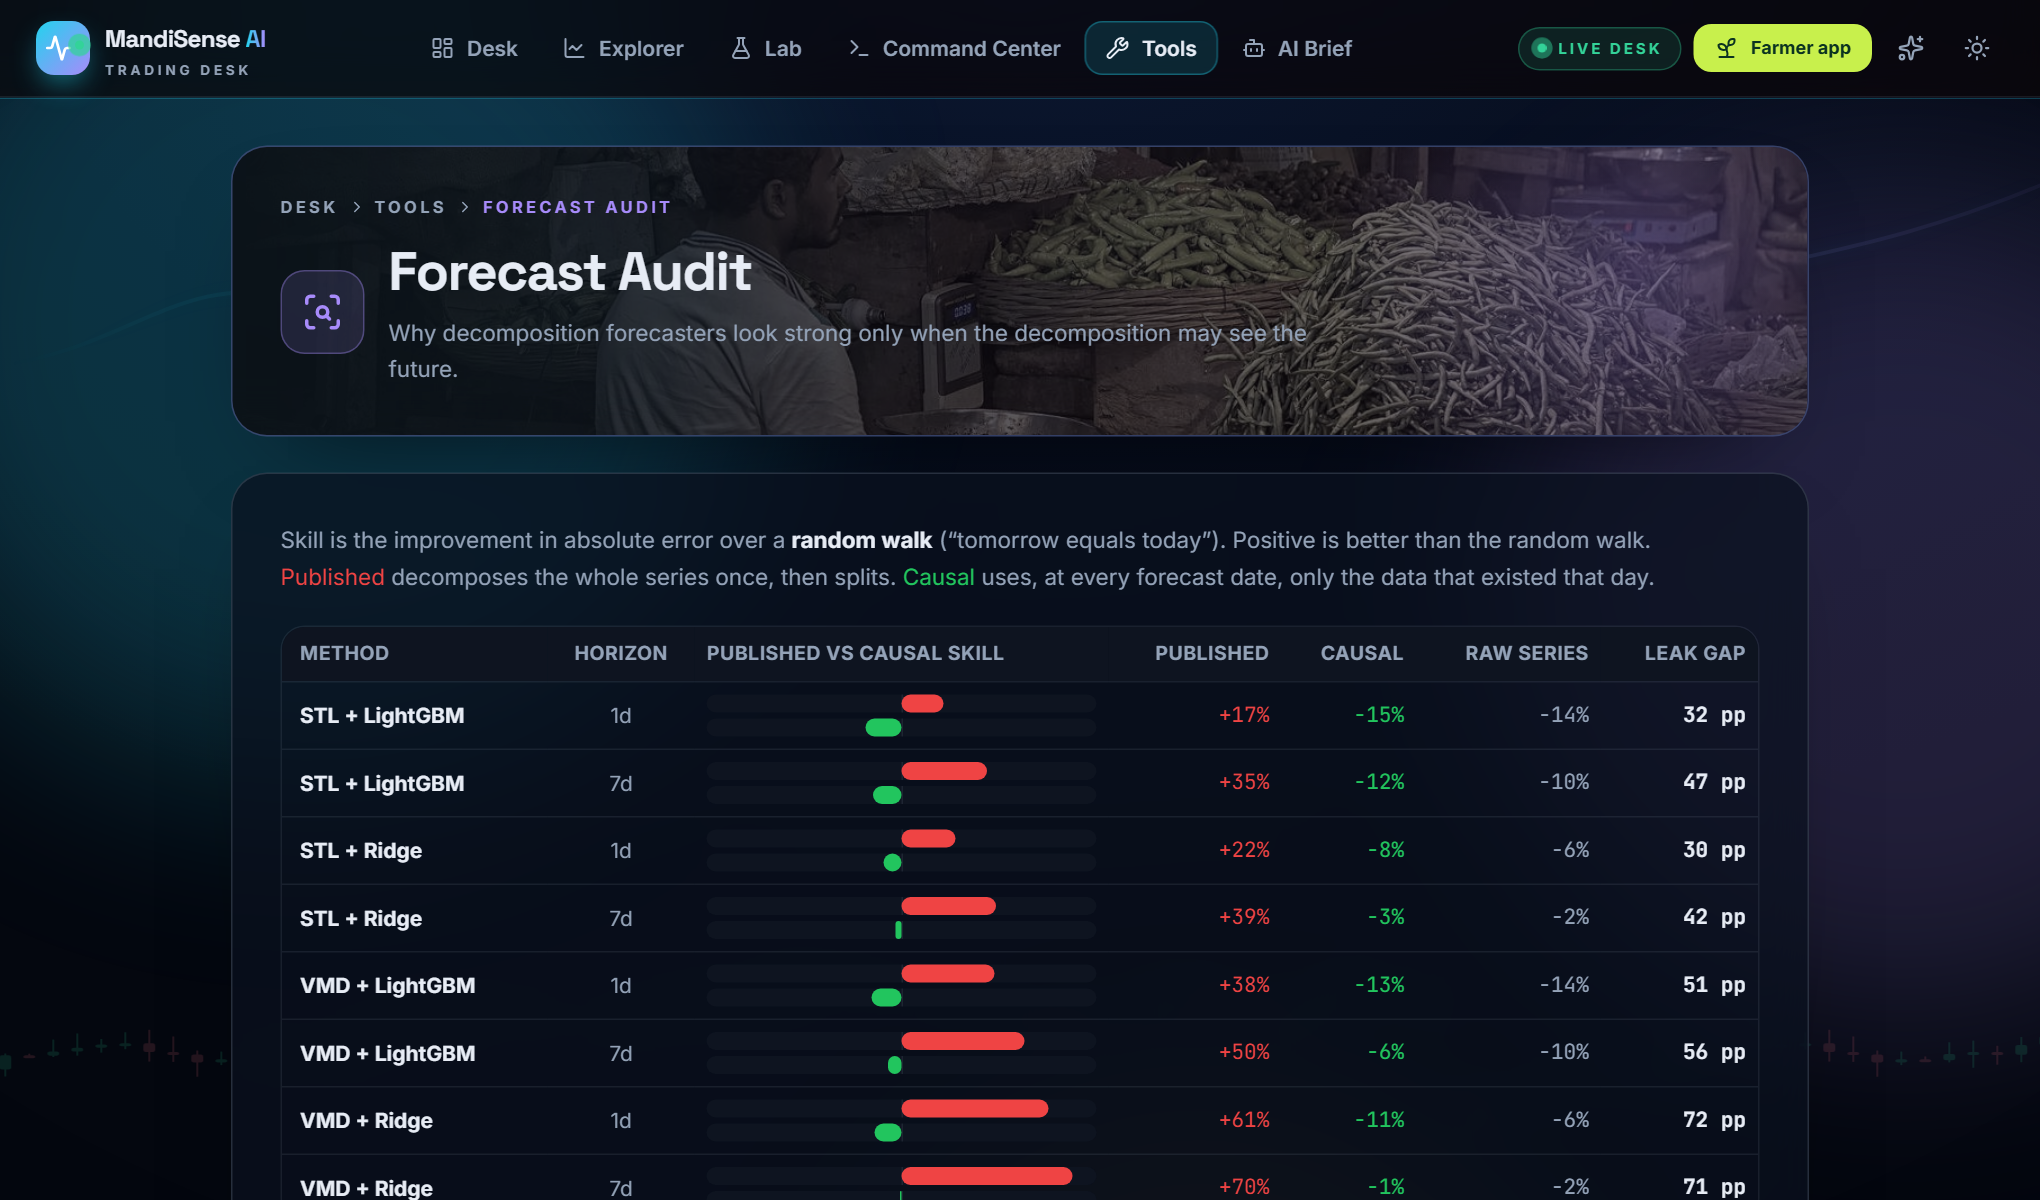
\includegraphics[width=0.93\linewidth]{figures/shot_w_audit.png}}\\[0.5mm]{\footnotesize (b) Forecast audit}
\caption{(a) Floor monitor: how often the revenue floor has held. (b) Forecast audit.}
\label{fig:sc-w-floormon}
\end{figure}

The monitor tracks, day by day, whether realised revenue stayed above the stated floor and shows the running violation rate against its target, so a drift in calibration is visible.

The audit compares each forecaster with the naive predictor on the days it was used and shows where it adds nothing.

\begin{figure}[!t]
\centering
\fbox{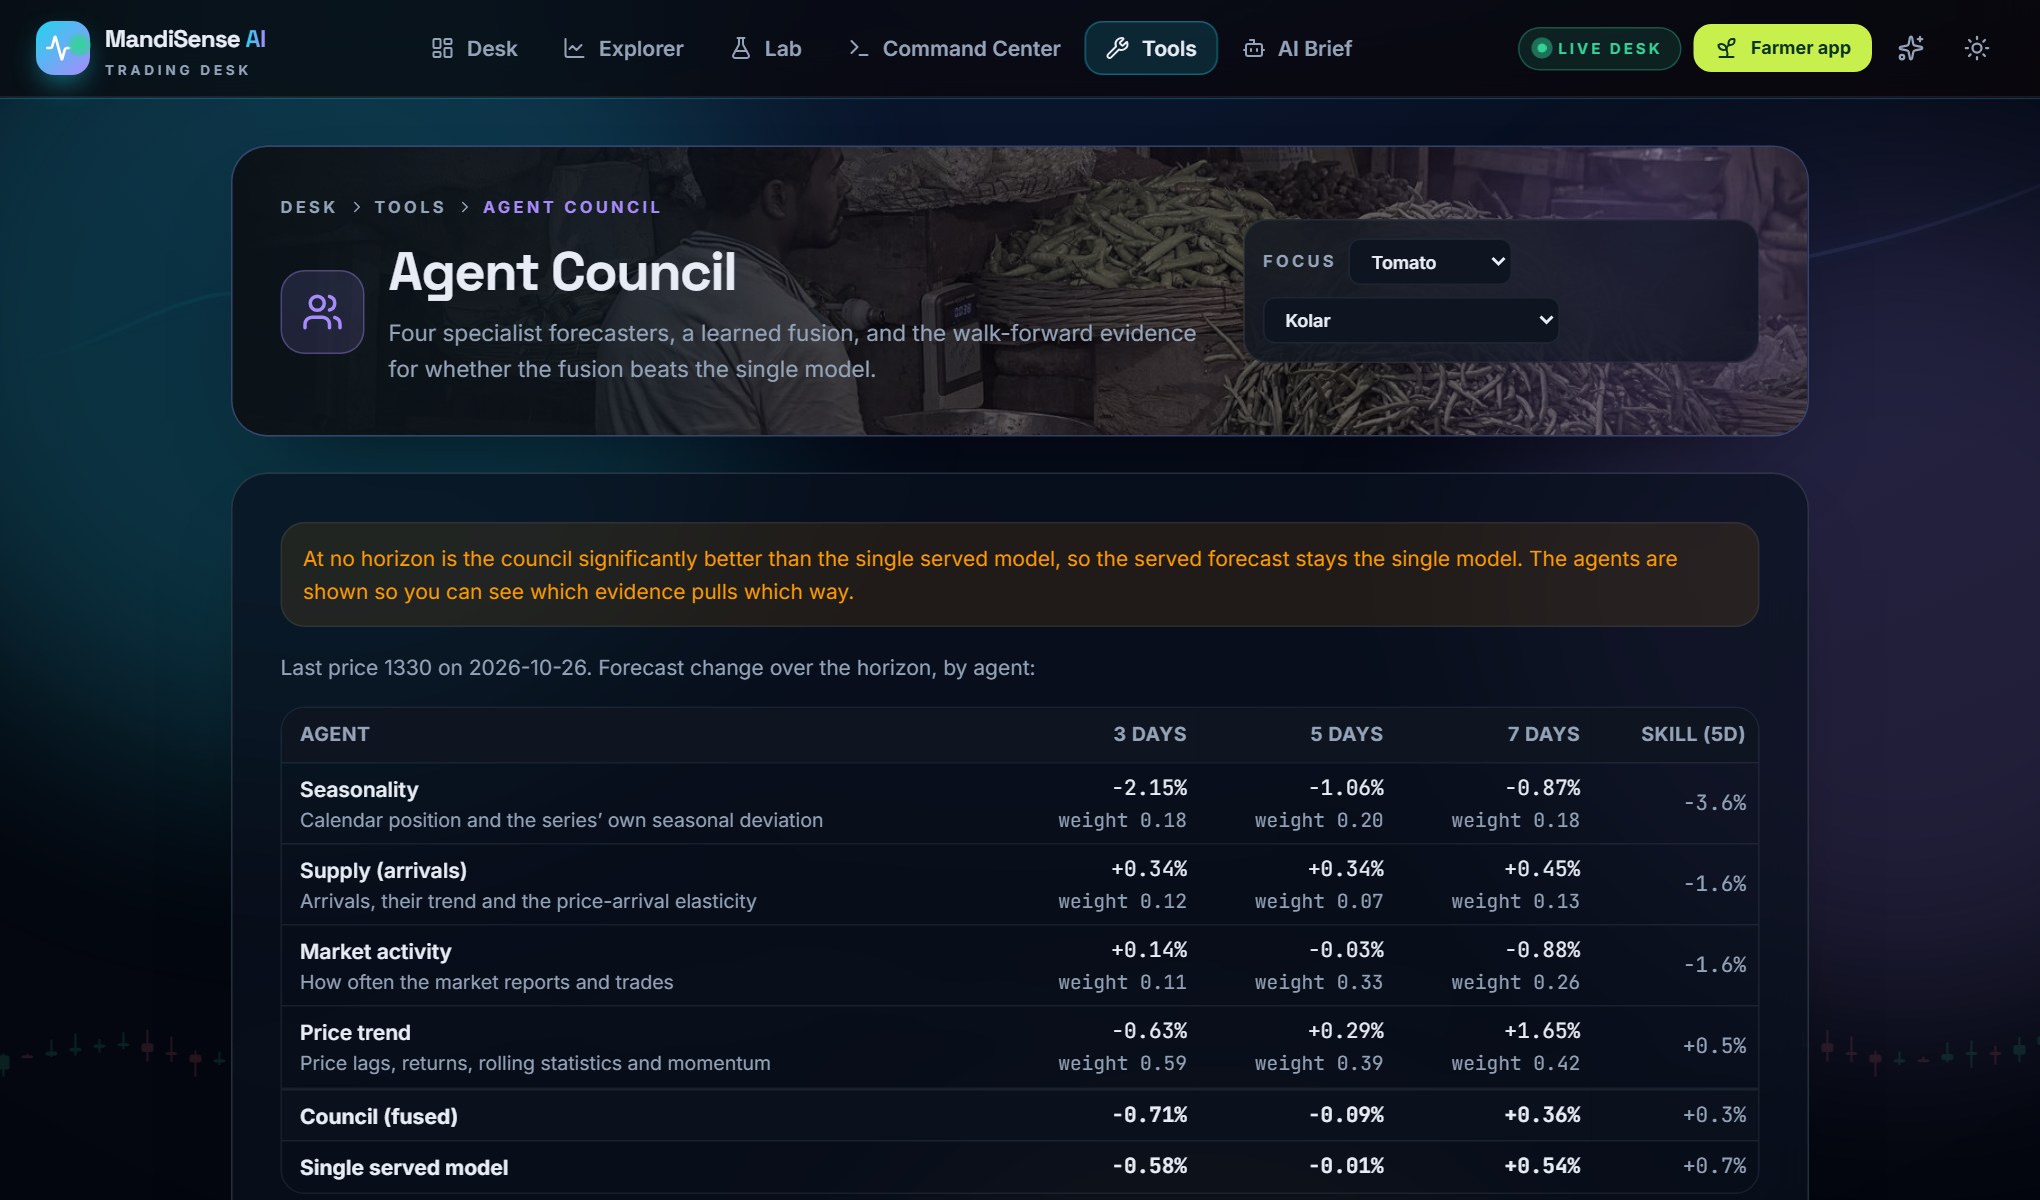
\includegraphics[width=0.93\linewidth]{figures/shot_w_council.png}}\\[0.5mm]{\footnotesize (a) Agent council: specialist forecasters and their weights}
\medskip
\fbox{
\includegraphics[width=0.93\linewidth]{figures/shot_w_explorer.png}}\\[0.5mm]{\footnotesize (b) Market explorer: any crop, any market, any period}
\caption{(a) Agent council: specialist forecasters and their weights. (b) Market explorer: any crop, any market, any period.}
\label{fig:sc-w-council}
\end{figure}

The council page shows the specialist forecasters and the weight each currently carries, the object of Section~\ref{sec:architecture}.

The explorer lets a user chart raw reported prices and arrivals, with gaps in reporting shown as gaps.

\begin{figure}[!t]
\centering
\fbox{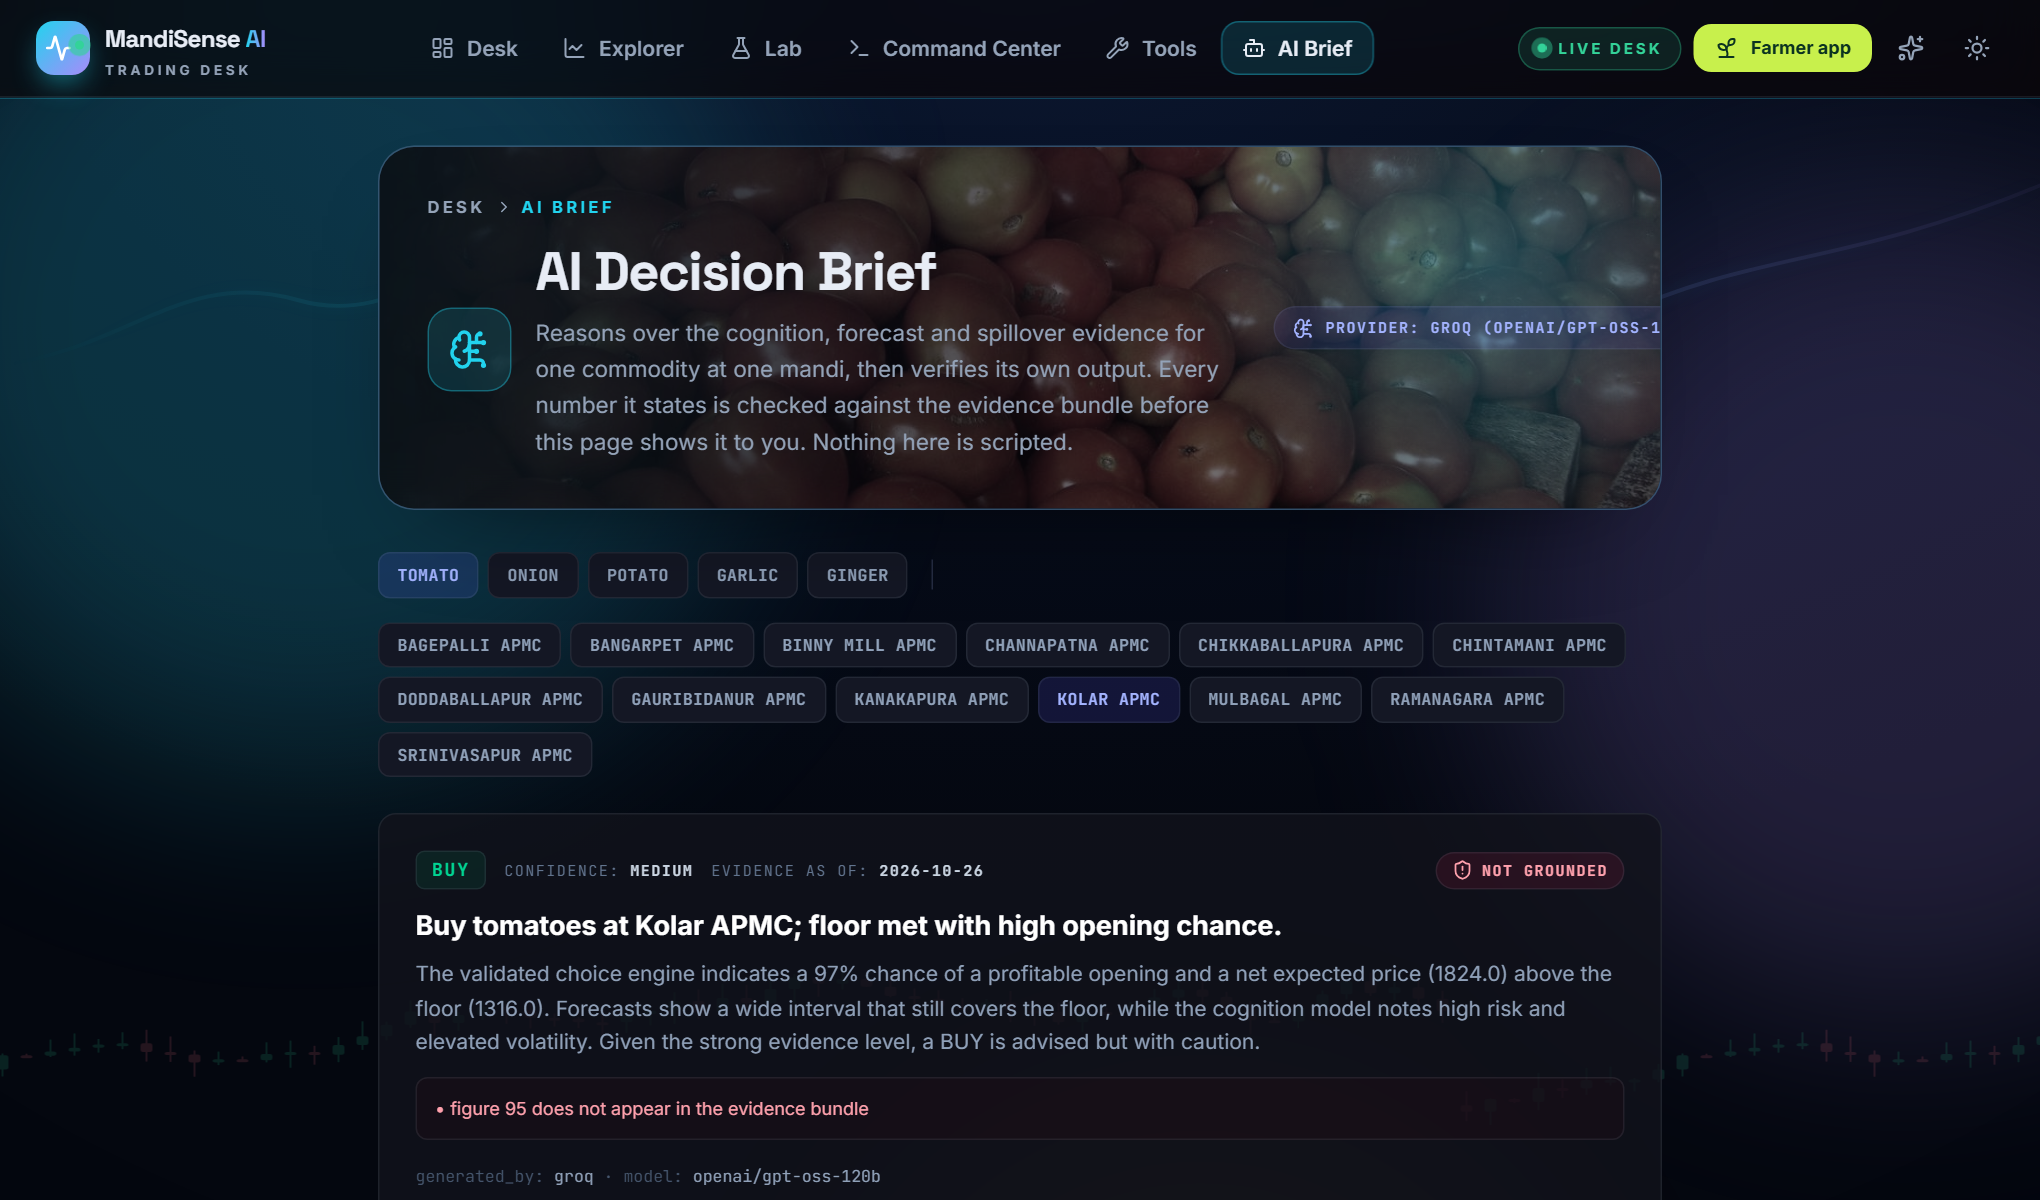
\includegraphics[width=0.93\linewidth]{figures/shot_w_aibrief.png}}\\[0.5mm]{\footnotesize (a) The AI brief: a written summary checked against the evidence}
\medskip
\fbox{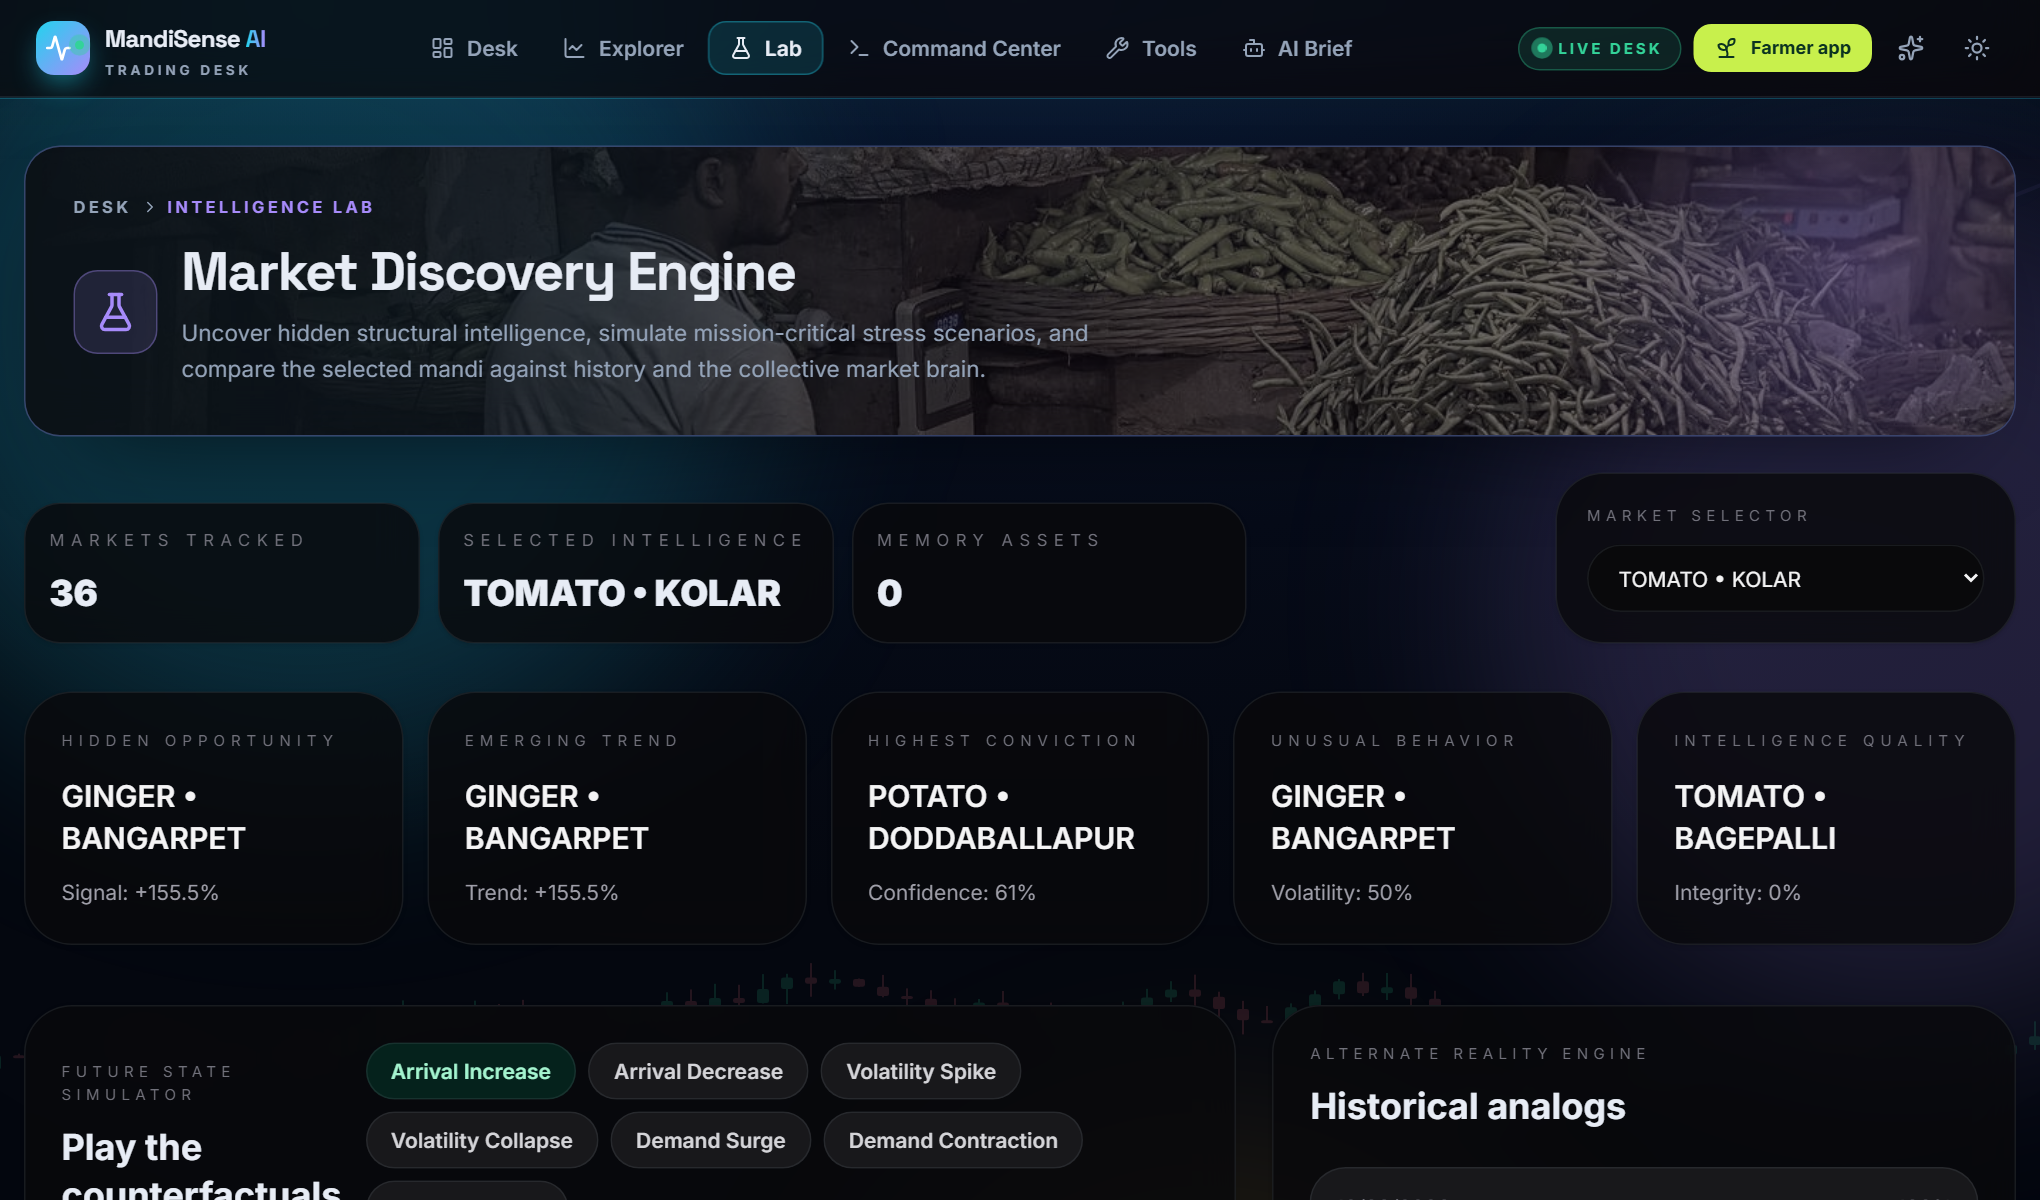
\includegraphics[width=0.93\linewidth]{figures/shot_w_lab.png}}\\[0.5mm]{\footnotesize (b) Intelligence lab: experiment summaries}
\caption{(a) The AI brief: a written summary checked against the evidence. (b) Intelligence lab: experiment summaries.}
\label{fig:sc-w-aibrief}
\end{figure}

The brief is written by the language model of Section~\ref{sec:llm} and every figure in it is checked against the evidence before it is shown. A brief that fails the check is discarded and the page falls back to a plain summary.

The lab page presents the experiment results of Chapter~\ref{ch:results} interactively.

\begin{figure}[!t]
\centering
\fbox{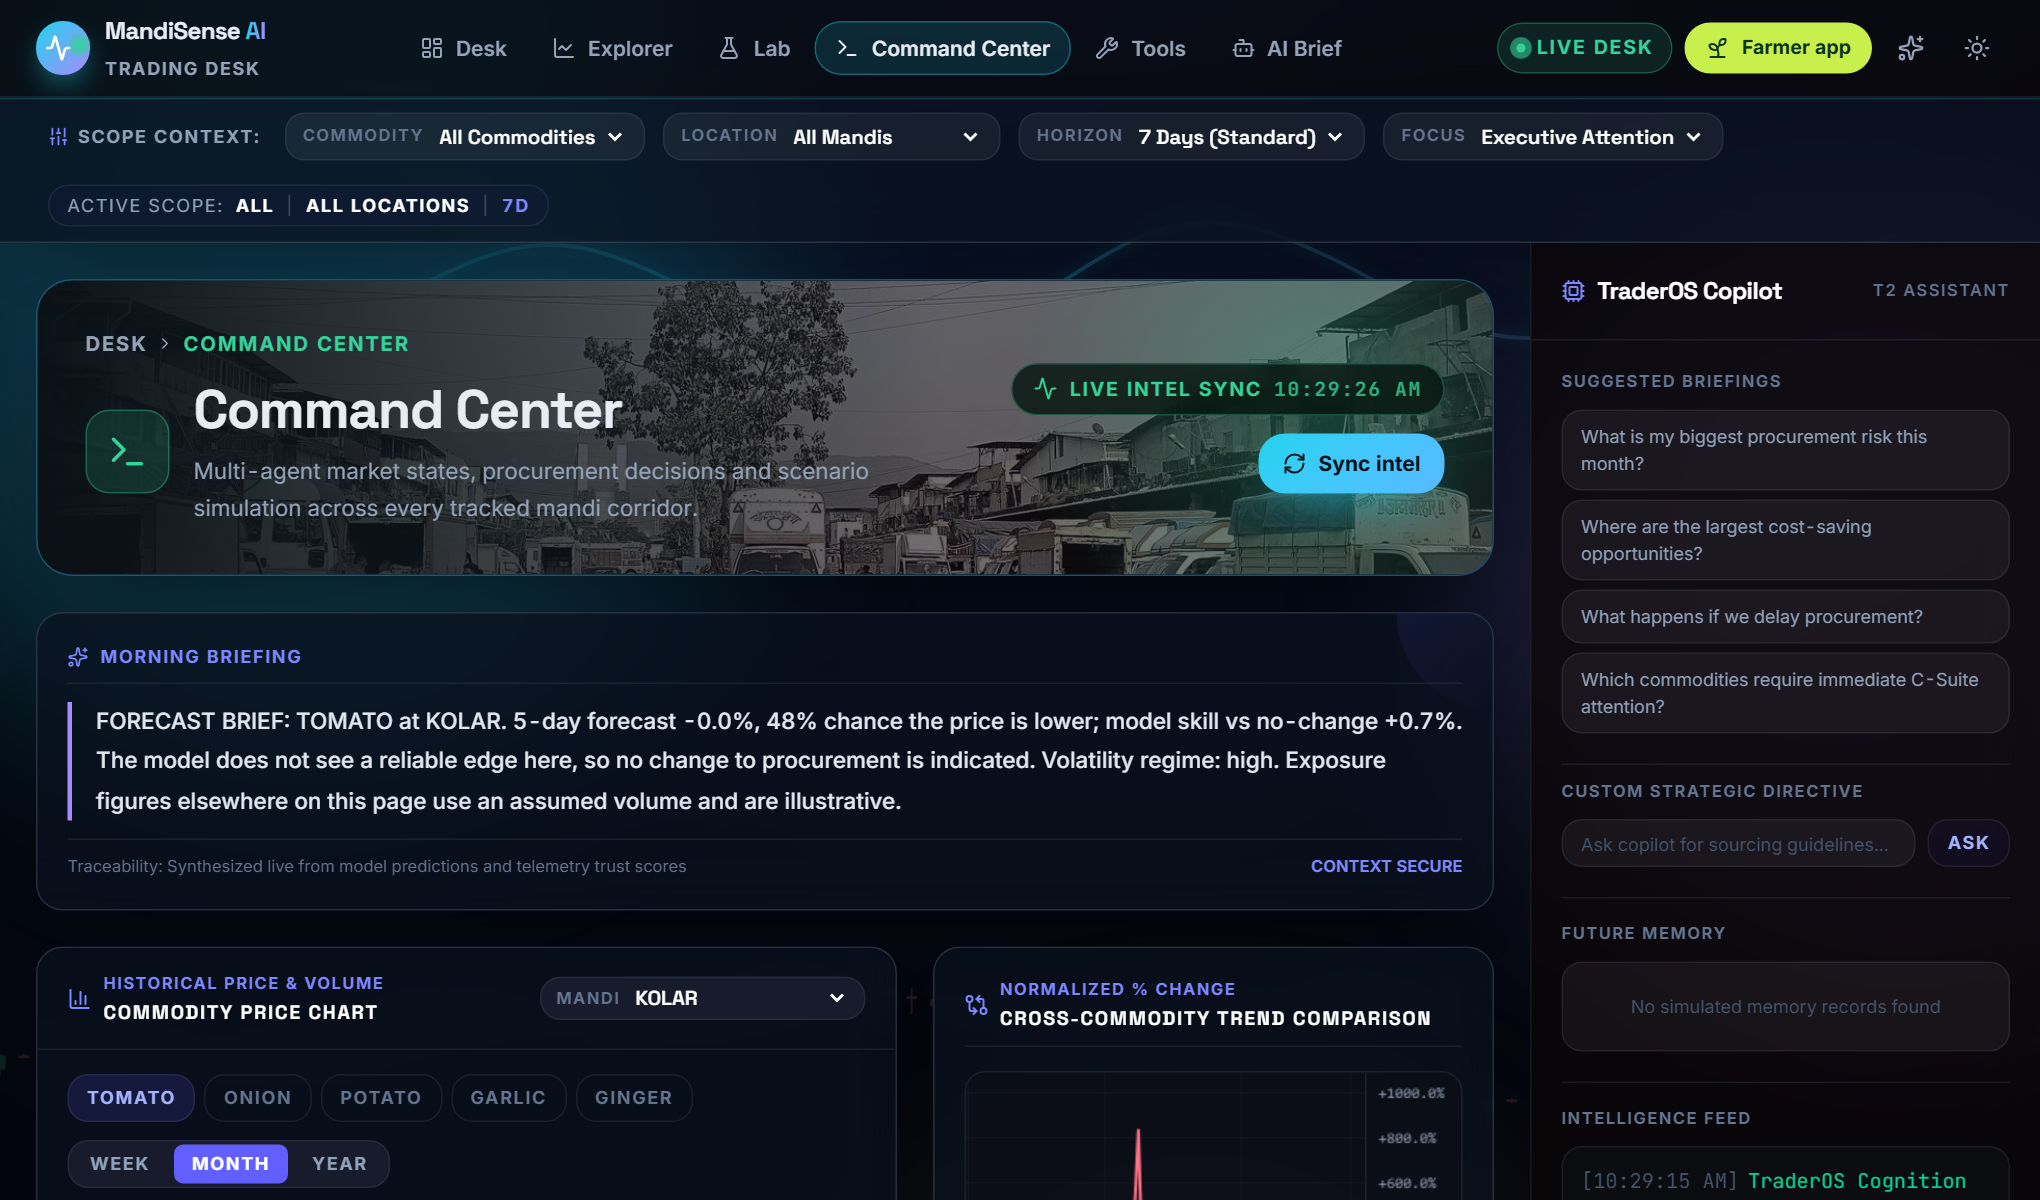
\includegraphics[width=0.93\linewidth]{figures/shot_w_terminal.png}}\\[0.5mm]{\footnotesize (a) Terminal view: dense prices for desk use}
\medskip
\fbox{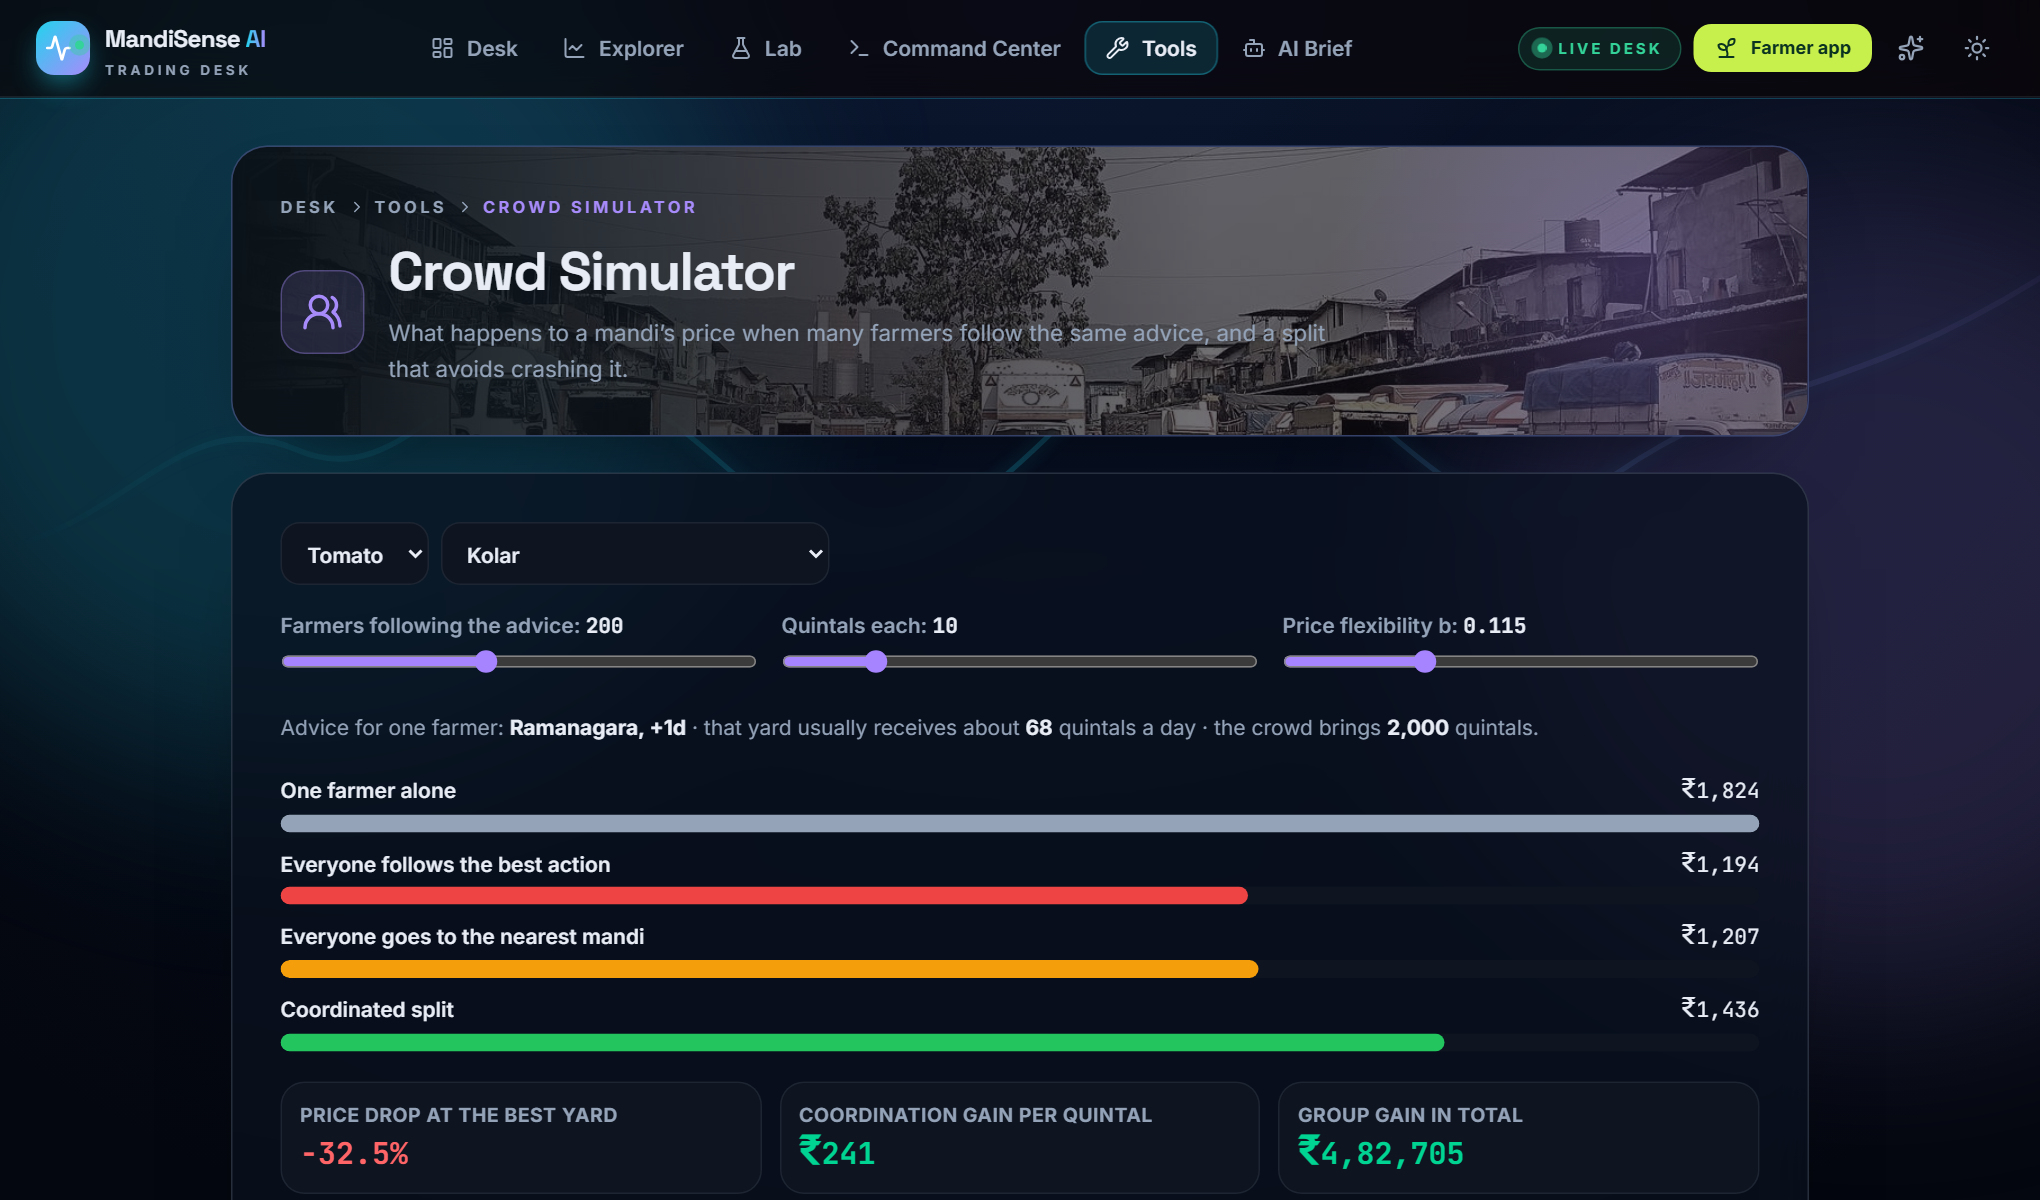
\includegraphics[width=0.93\linewidth]{figures/shot_w_crowd.png}}\\[0.5mm]{\footnotesize (b) Crowd simulator: what happens when many farmers follow the same advice}
\caption{(a) Terminal view: dense prices for desk use. (b) Crowd simulator: what happens when many farmers follow the same advice.}
\label{fig:sc-w-terminal}
\end{figure}

A compact table of the latest price per market, intended to stay open beside other work.

The simulator raises the share of farmers following the advice and shows the net revenue under four policies, using a stated price flexibility (Section~\ref{sec:insight-method}).

\begin{figure}[!t]
\centering
\fbox{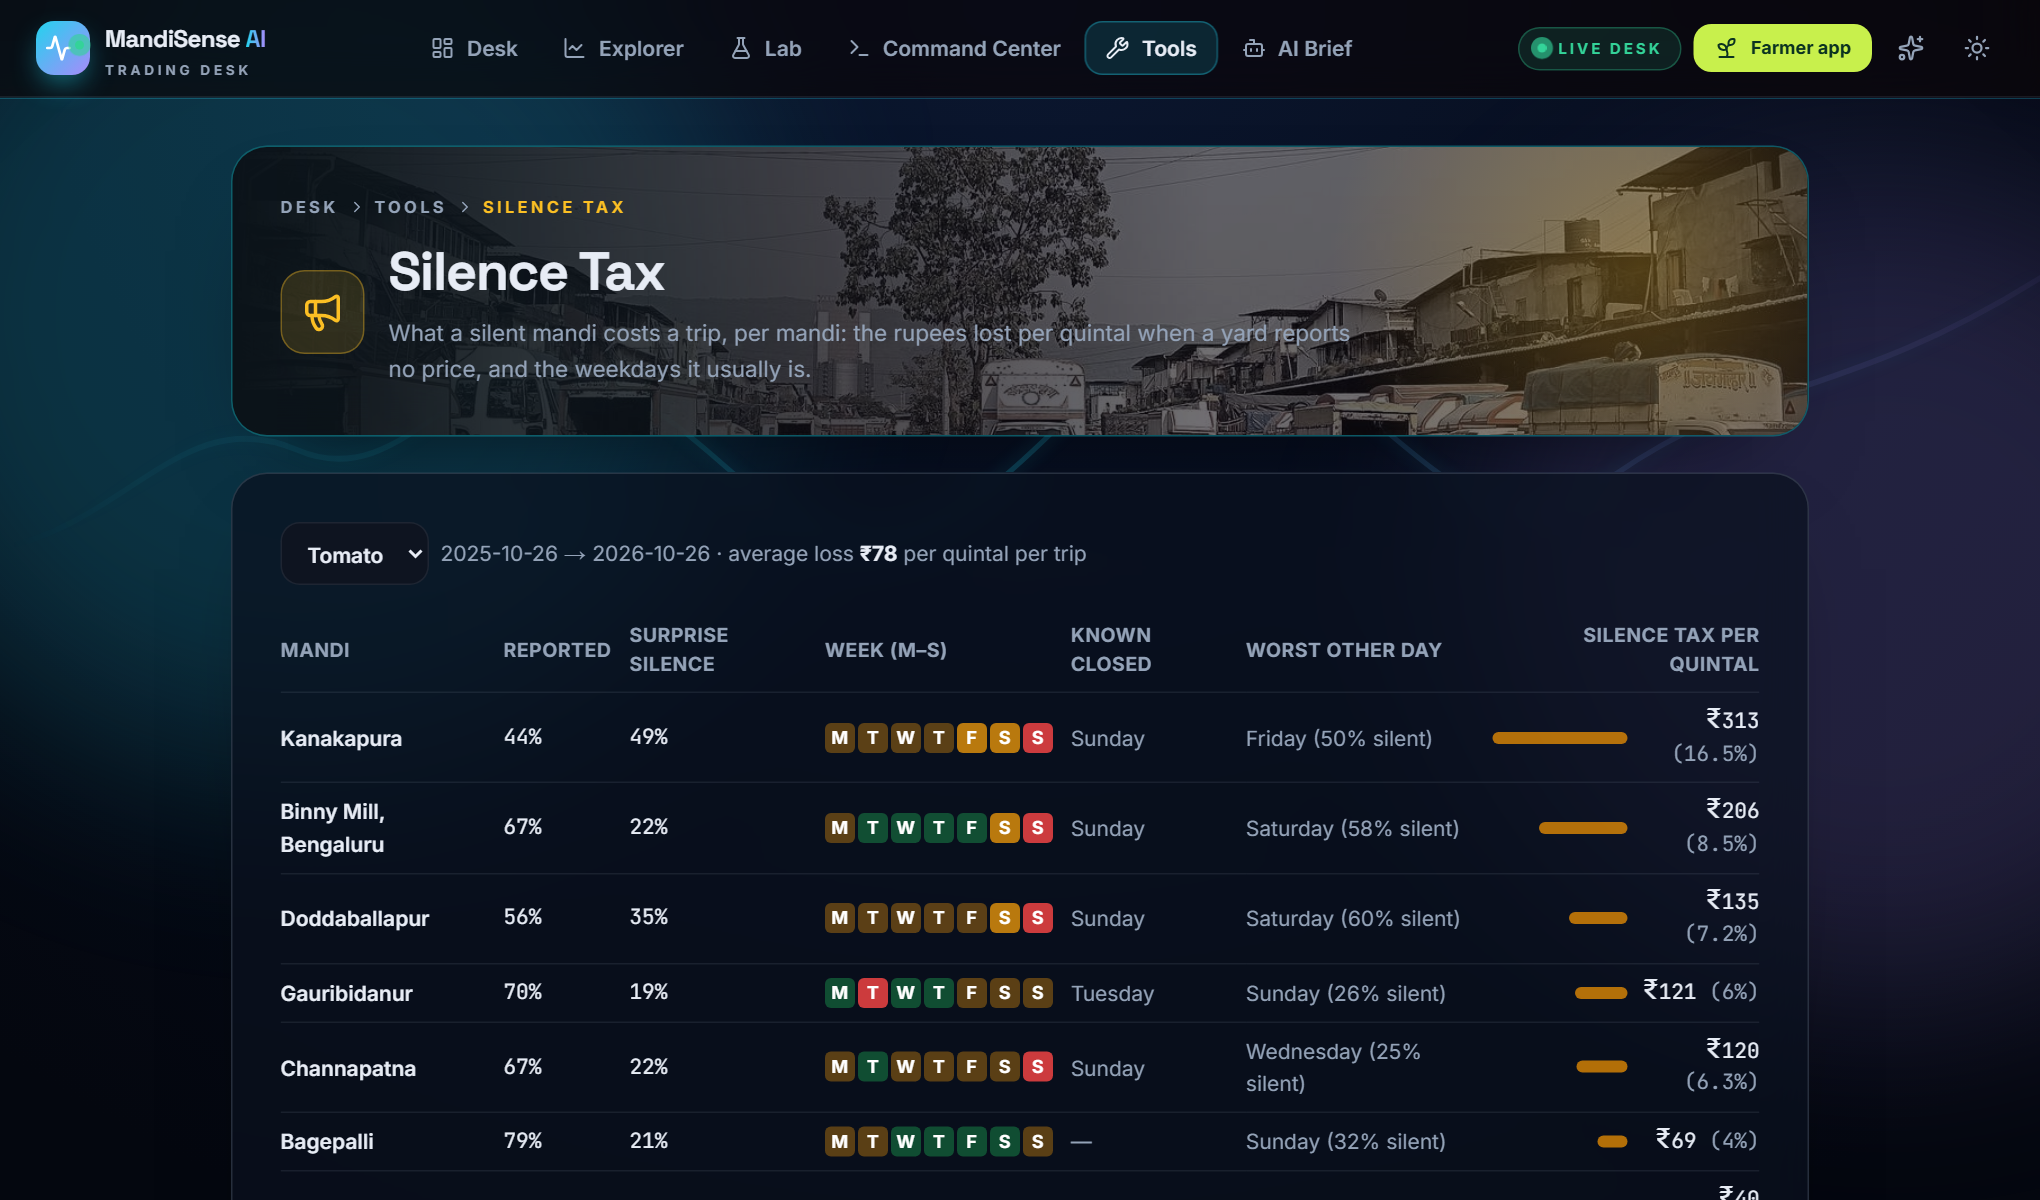
\includegraphics[width=0.93\linewidth]{figures/shot_w_repval.png}}\\[0.5mm]{\footnotesize (a) Reporting value (silence tax): what a market's silence costs}
\medskip
\fbox{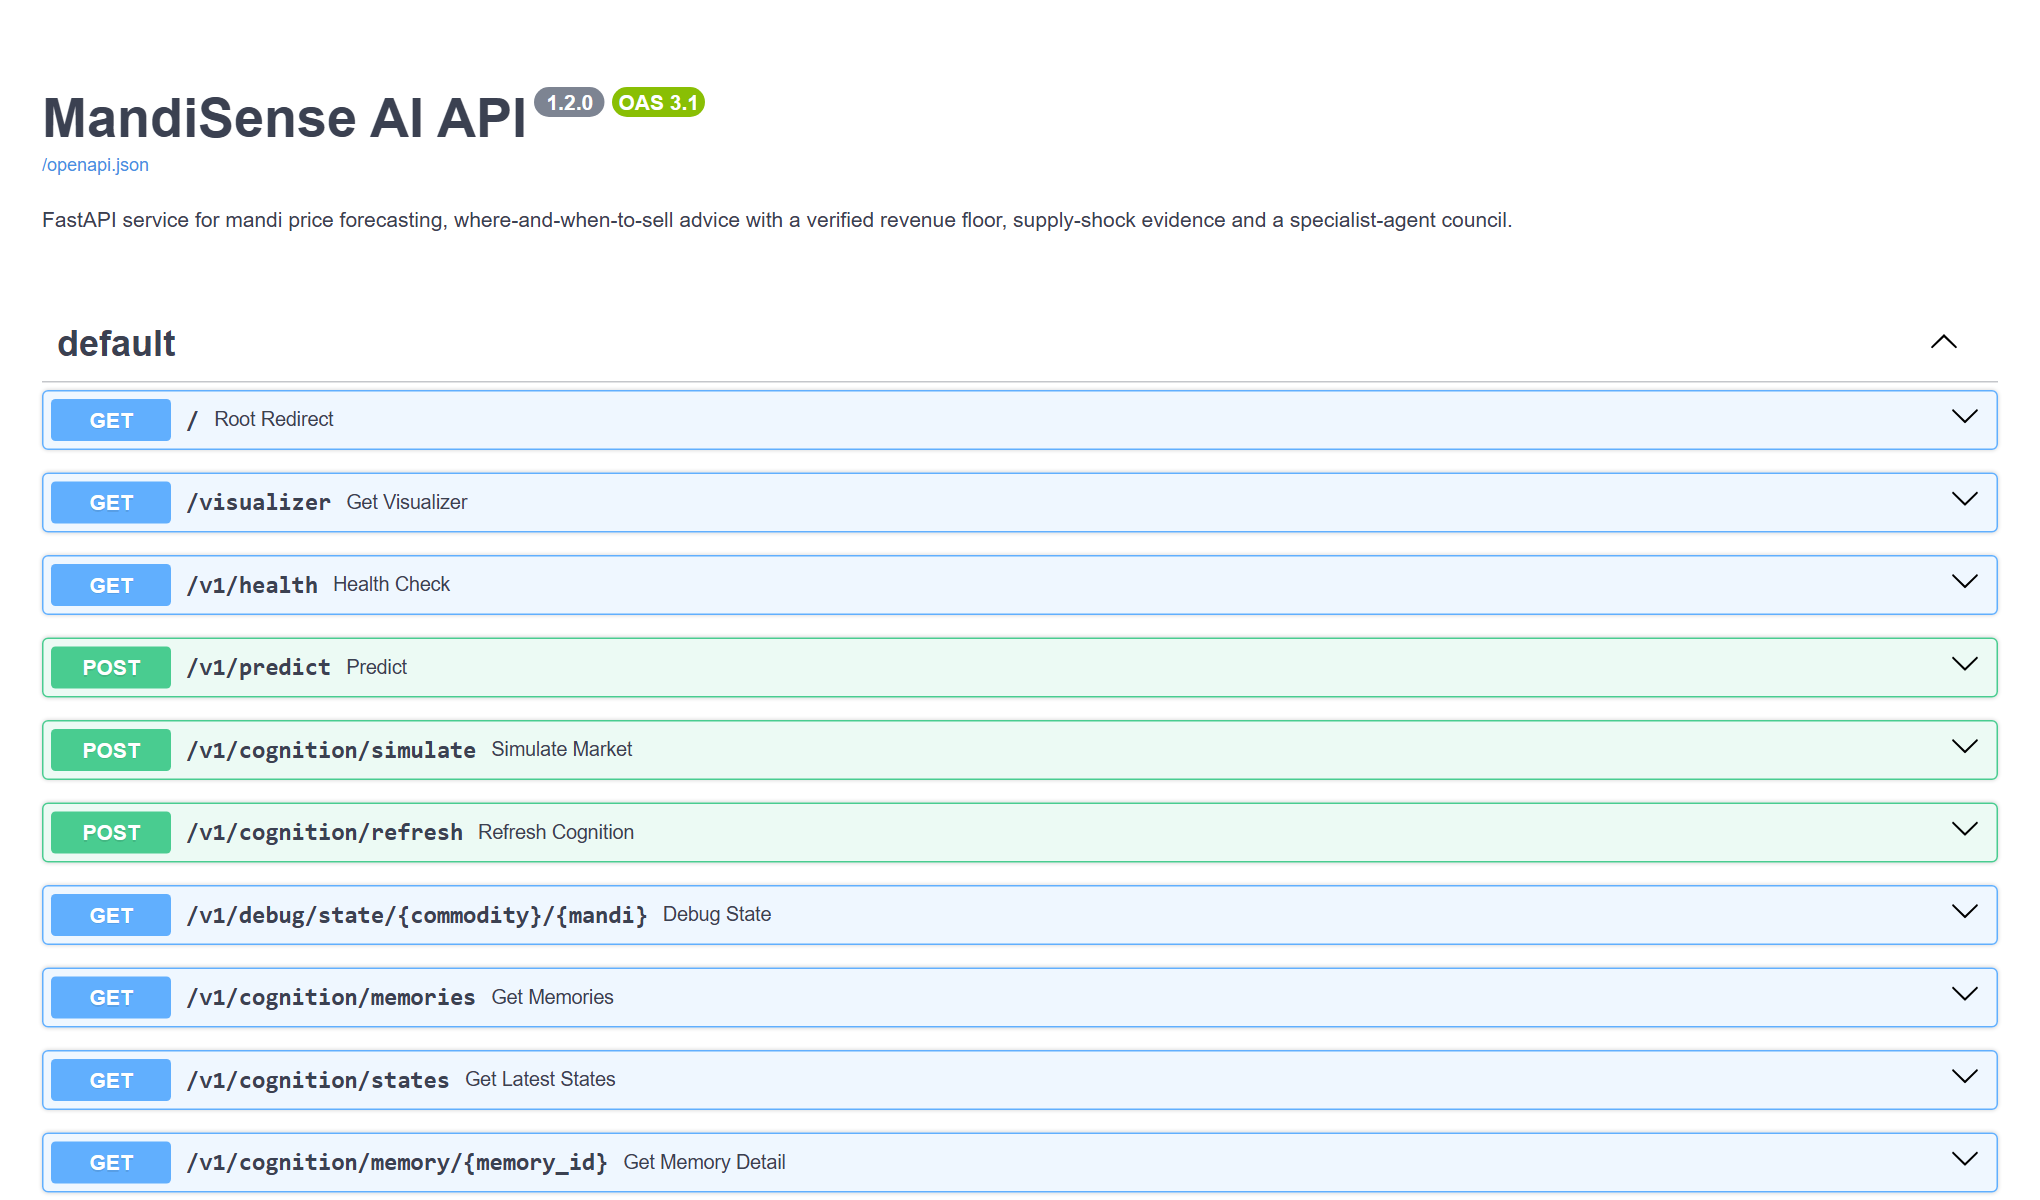
\includegraphics[width=0.93\linewidth]{figures/shot_w_docs.png}}\\[0.5mm]{\footnotesize (b) The interactive API documentation}
\caption{(a) Reporting value (silence tax): what a market's silence costs. (b) The interactive API documentation.}
\label{fig:sc-w-repval}
\end{figure}

The page estimates, per mandi, the revenue lost on days when a market did not report, which is the silence tax of Section~\ref{sec:insight-method}.

Every endpoint is documented automatically from the code, with a form to try it; the service is described in Section~\ref{sec:service-app}.


\section{Testing and Validation}
\label{sec:testing-validation}

\subsection{Strategy}

Testing has four levels. Unit tests check individual functions, including the SPO+ properties (non-negative, zero at the truth, upper bound on regret, respects the offered set, matches brute force) and the conformal quantile. Leakage tests perturb future values and require features to be unchanged, and corrupt not-yet-known outcomes and require the floor to be unchanged. Integration tests exercise the API routers against the real data layer. A results-document test checks that every figure linked from the generated results exists, that no unfilled value leaked, and that headline numbers match the source tables. A continuous-integration workflow runs the Python and web tests on each push.

\subsection{Coverage and outcome}

\begin{table}[!t]
\centering
\caption{Test inventory}
\label{tab:tests}
\small
\begin{tabular}{|l|p{6.4cm}|l|}
\hline
\textbf{Layer} & \textbf{Content} & \textbf{Tool} \\ \hline
Application tests & 669 tests (all passing on 29 October 2026) across engines, API, trader and farmer features, council, shock, spillover, chat, results document, insight features and the digest & pytest \\ \hline
Research tests & Core losses, models, pipeline, leakage; need the separate research environment with PyTorch & pytest \\ \hline
Web tests & 11 copy and registry tests for the three languages and the tool registry & vitest \\ \hline
UI smoke test & 60 checks: every API endpoint and page the application depends on, including the five insight endpoints and the two new trader tools (\texttt{scripts/smoke\_ui.py}) & headless Chrome \\ \hline
Fresh-clone check & Clone, install, run pipeline subset, run tests & manual, repeated \\ \hline
\end{tabular}
\end{table}

\noindent\textbf{Negative outcomes.} The fresh-clone check initially failed (Table~\ref{tab:challenges}); the three research-test modules cannot be collected in the application environment because PyTorch is installed only in the research environment, which is by design but means a single \texttt{pytest} call at the repository root reports three collection errors. The deployment configuration (Docker, Render) is provided but has not been verified end to end, and no claim about a live deployment is made in this thesis.
